\documentclass{article}
\setlength{\parskip}{10pt}

\usepackage[a4paper, left=3cm, right=3cm, top=30mm, bottom=30mm]{geometry}
\usepackage{blindtext}
\usepackage[spanish]{babel}
%\usepackage{titlesec}
\usepackage{graphicx}
\usepackage{amssymb} % para introducir símbolos como el tick
\usepackage{xcolor}
\usepackage{wrapfig}
\usepackage{subcaption}
\usepackage[hidelinks]{hyperref}
\usepackage{url}
\usepackage[super,comma]{natbib}

\usepackage{listings}
\lstnewenvironment{codigo}{\lstset{language=C, basicstyle=\small\ttfamily, frame=single, showstringspaces=false}}{}

\setcitestyle{super,aysep={},citesep={,}}

\begin{document}
\begin{titlepage} 

\newlength{\centeroffset}
\setlength{\centeroffset}{-0.5\oddsidemargin}
\addtolength{\centeroffset}{0.5\evensidemargin}
\thispagestyle{empty}

\noindent\hspace*{\centeroffset}
\begin{minipage}{\textwidth}

\centering

\includegraphics[width=0.9\textwidth]{imagenes/logos/logo_ugr.jpg}\\[1.4cm]

\textsc{\Large TRABAJO FIN DE GRADO\\[0.2cm]}
\textsc{GRADO EN INGENIERÍA INFORMÁTICA}\\[1cm]

% Título
{\Huge\bfseries GoShopp\\}
\noindent\rule[-1ex]{\textwidth}{3pt}\\[3.5ex]
{\large\bfseries Aplicación Móvil para Gestionar la Lista de la Compra}
\end{minipage}\\[1cm]

\centering

\includegraphics[width=0.35\textwidth]{imagenes/logos/logo.png}

\vspace{1cm}
\noindent\hspace*{\centeroffset}\begin{minipage}{\textwidth}
\centering

\textbf{Autor}\\ {Pablo Muñoz Castro}\\[2.5ex]
\textbf{Tutor}\\ {Juan José Escobar Pérez}\\[1cm]


\includegraphics[width=0.3\textwidth]{imagenes/logos/logo_etsiit.png}\\[0.1cm]

\textsc{Escuela Técnica Superior de Ingenierías Informática y de Telecomunicación}\\
\textsc{---}\\Granada, julio de 2023

\end{minipage}

\end{titlepage}
\thispagestyle{empty}

\noindent{\textbf{Resumen}}\\

El presente proyecto consiste en el desarrollo de una aplicación móvil multiplataforma, es decir, diseñada tanto para el sistema operativo Android como para iOS, y cuyo objetivo es facilitar la tarea de gestionar listas de la compra, tanto personales como entre grupos de conocidos. Con esto, se pretende que cada usuario pueda añadir productos a sus listas privadas o a otros grupos en cualquier momento desde su dispositivo móvil, de forma que cuando uno de los integrantes vaya a hacer la compra, no falte nada. La aplicación también cuenta con una sección de chat, que permite a los usuarios de un grupo poder comunicarse entre ellos a la hora de crear las diferentes listas y unirse al grupo que deseen o crear uno nuevo. Adicionalmente, también se permite a los usuarios escanear el contenido de un ticket de la compra, ya sea mediante la cámara o mediante una imagen obtenida del dispositivo, para así poder añadir productos a una lista de una manera mucho más rápida y sencilla. Esto supone que el propio programa tiene la capacidad de reconocer textos y procesarlos para que, simplemente con una imagen del recibo de la compra, se añadan cada uno de los productos como si se hiciese manualmente. Para desarrollar todo lo mencionado, se ha implementado la aplicación utilizando Flutter, un entorno de trabajo que permite desarrollar simultáneamente aplicaciones tanto para Android como para iOS, además de plataformas externas como Firebase, utilizada en el desarrollo de aplicaciones web y  móviles y, desde hace un tiempo, adquirida por Google.

\vspace{0.7cm}

\noindent{\textbf{Palabras clave}: Flutter, Dart, Firebase, Aplicación móvil, Listas de la compra, Chat, Reconocimiento de textos.}\\

\clearpage

\thispagestyle{empty}

\noindent{\textbf{Abstract}}\\

The present project consists of the development of a multi-platform mobile application, meaning it is designed for both the Android and iOS operating systems. Its objective is to make easier the task of managing shopping lists, both personal and group. Then, each user can add products to their personal lists or to the lists of a group they belong to at any time from their mobile device, so that when one of the members goes shopping, nothing is missing. The application also has a chat section, which allowing group users to communicate with each other when creating the different lists, as well as allowing them to join any group they desire or create a new one. Additionally, users also are able to scan the contents of a purchase receipt, either using the camera or by uploading an image from their device, to add products to a list in a much faster and easier way. This means that the program itself has the ability to recognize texts and process them so that, simply with an image of the purchase receipt, each of the products is added as if it were done manually. To develop all of the aforementioned, the application has been implemented using Flutter, a development environment that allows for the simultaneous development of applications for Android and iOS, and external platforms such as Firebase, used in the development of web and mobile applications, managed by Google.

\vspace{0.7cm}

\noindent{\textbf{Keywords}: Flutter, Dart, Firebase, Cross-platform mobile application, Shopping lists, Chat, Text recognition}\\

\newpage

\noindent\rule[-1ex]{\textwidth}{2pt}\\[4.5ex]

Yo, \textbf{Pablo Muñoz Castro}, alumno de la titulación GRADO EN INGENIERÍA INFORMÁTICA de la \textbf{Escuela Técnica Superior de Ingenierías Informática y de Telecomunicación de la Universidad de Granada}, con DNI 77557076H, autorizo la ubicación de la siguiente copia de mi Trabajo Fin de Grado en la biblioteca del centro para que pueda ser consultada por las personas que lo deseen.

\vspace{2cm}

\noindent Fdo: Pablo Muñoz Castro

\vspace{2cm}

\begin{flushright}
Granada a 4 de julio de 2023.
\end{flushright}

\newpage

\noindent\rule[-1ex]{\textwidth}{2pt}\\[4.5ex]

D. \textbf{Juan José Escobar Pérez}, profesor del Departamento Lenguajes y Sistemas Informáticos de la Universidad de Granada.


\vspace{0.5cm}

\textbf{Informa:}

\vspace{0.5cm}

Que el presente trabajo, titulado \textit{\textbf{Aplicación Móvil para Gestionar la Lista de la Compra}}, ha sido realizado bajo su supervisión por \textbf{Pablo Muñoz Castro}, y autorizo la defensa de dicho trabajo ante el tribunal que corresponda.

\vspace{0.5cm}

Y para que conste, expido y firmo el presente informe en Granada a 4 de julio de 2023.

\vspace{2cm}

\textbf{El tutor:}

\vspace{1cm}

\noindent \textbf{Juan José Escobar Pérez}

\newpage

\section*{Agradecimientos}
\thispagestyle{empty}

       \vspace{1cm}

Quisiera aprovechar este espacio para expresar mi profundo agradecimiento a todas aquellas personas que contribuyeron de manera significativa en la realización de este trabajo de fin de grado. Su apoyo, orientación y aliento fueron fundamentales para culminar este importante logro en mi trayectoria académica:

A mi tutor, Juan José, por su inestimable guía y dedicación a lo largo de estos meses. Agradezco sinceramente su apoyo constante y su capacidad para ofrecer nuevas posibilidades e ideas en el desarrollo de la aplicación.

A todos los profesores que, durante estos cuatro años, se han esforzado en brindar el máximo de sus posibilidades en mi aprendizaje y por proporcionarme las herramientas intelectuales necesarias para desarrollar este proyecto.

A mis compañeros de clase, más bien amigos, quienes me han brindado su apoyo incondicional durante esta etapa. Sus palabras de aliento, su ayuda en estos cuatro años y, principalmente, los momentos de distracción fueron esenciales para mantener mi motivación y confianza en mí mismo, especialmente en una época muy complicada como fue la pandemia.

A mi familia, por su apoyo constante y porque siempre se han esforzado al máximo en todos los aspectos para que nunca me faltase nada, les agradezco su amor, comprensión y paciencia.

A mi novia, por ser mi mayor soporte emocional y por su respaldo constante, que ha sido fundamental para superar los desafíos y obstáculos que surgieron en este camino.

Por ultimo, quiero destacar mi propio esfuerzo y dedicación en este proyecto, el cual se ha convertido tanto en un desafío personal, como en una experiencia de aprendizaje que me ha permitido complementar mis habilidades como desarrollador de software, así como aprender nuevas habilidades y tecnologías.

\newpage
\cleardoublepage

\tableofcontents

\newpage

\listoffigures
%\listoftables

\newpage

\section{Introducción}

En la era digital en la que se vive, la gestión eficiente de las tareas diarias se ha vuelto imprescindible para optimizar el tiempo y simplificar las vidas. Una de las actividades más comunes es hacer la compra, en la cual es frecuente no acordarse o no tener claro si falta algún producto. Por ejemplo, es común olvidar algo importante en el supermercado o comprar algo que otra persona ya había adquirido sin avisar. Para solucionar este problema se ha desarrollado \textit{GoShopp}, una aplicación móvil diseñada para ayudar a gestionar las listas de la compra de manera rápida, eficiente e incluso colaborativa.

Esta aplicación tiene como objetivo permitir al usuario crear múltiples listas de la compra, tanto individuales como cooperativas, para diferentes ocasiones y grupos, como una lista para la compra familiar o para una quedada con amigos. El objetivo de estas listas cooperativas es que cada uno de los miembros del grupo tenga acceso a ellas y pueda añadir y eliminar productos o marcarlos como comprados, de forma que cuando alguien vaya a hacer la compra, no falte nada por adquirir o pueda tener en cuenta qué productos ya se ha comprado. Se pueden nombrar las listas de acuerdo a las preferencias de los usuarios y añadir una descripción, lo que facilita la búsqueda y selección de elementos específicos.

La funcionalidad de \textit{GoShopp} no se limita solo a la creación de listas individuales, ya que esto podría hacerse fácilmente anotando los productos en papel o digitalmente en un bloc de notas, por ejemplo. La aplicación, además de permitir esto, se centra en la posibilidad de compartir las listas de la compra con grupos de allegados, como familiares, compañeros de piso o amigos, lo que facilita la colaboración y la coordinación de compras conjuntas. Para ello, también se implementará una funcionalidad de chat entre usuarios, permitiendo crear, borrar y participar en grupos, lo que permite la comunicación sin necesidad de salir de la aplicación.

Para resaltar la facilidad de uso del software desarrollado, \textit{GoShopp} contará con una funcionalidad que permitirá a los usuarios escanear los tickets de compra. Esta característica aprovecha la inteligencia artificial para reconocer los textos en las imágenes, ya sea capturadas desde la cámara del dispositivo o seleccionadas desde la galería, y de esta manera detecta automáticamente los productos mencionados en ellos y los añade a la lista seleccionada de forma más eficiente que si se hiciera manualmente.

En resumen, en un mundo cada vez más digitalizado y acelerado, el uso de aplicaciones móviles como \textit{GoShopp} se ha vuelto esencial para optimizar las actividades cotidianas. En este caso, no solo ahorrará tiempo y esfuerzo, sino que también mejorará la experiencia de compra al evitar olvidos o compras innecesarias, lo que permitirá organizar las tareas de manera más eficiente, colaborar con otros y mantener un control más preciso de los gastos.

Principalmente, la idea de comenzar a desarrollar una aplicación como la que se plantea surgió durante el tercer año de carrera, donde en una de las asignaturas se solicitó la entrega de una aplicación web, bastante básica, para gestionar las listas de la compra. La idea en sí resultó interesante, pues como se ha mencionado anteriormente, es un problema real el olvidarse de algún producto al ir de compras o comprar uno que ya se adquirió previamente. Una aplicación de este tipo podría solucionar no solo un problema de efectividad y organización, sino también uno económico.

Después de realizar dicha práctica, se planteó que podría ser más útil si, en lugar de una aplicación web, se desarrollara como una aplicación móvil. Esto permitiría tenerla en cualquier dispositivo y acceder a ella desde cualquier lugar y en cualquier momento. De esta forma, cuando se tenga la idea de comprar un producto, se puede añadir a la lista correspondiente, y cuando un miembro del grupo vaya a hacer la compra, tendrá toda la información sobre lo que se debe adquirir. Además de eso, surgió la posibilidad de implementar un chat entre usuarios, para evitar tener que salir de la aplicación y utilizar otras aplicaciones de mensajería para comunicarse con los miembros del grupo. De esta manera, todo estaría al alcance en la propia aplicación.

\subsection{Objetivos}

En el marco de este proyecto de desarrollo, se plantearon una serie de objetivos que serán la piedra angular de nuestro trabajo. Estos objetivos, cuidadosamente establecidos y respaldados por una planificación detallada, se centran en crear una solución innovadora y eficiente para la gestión de listas de compras. El objetivo principal es brindar a los usuarios una herramienta versátil y fácil de usar que les permita organizar y administrar sus compras de manera efectiva.

A continuación, se presentan los objetivos principales que la aplicación desarrollada deberá cumplir y que serán abordados a lo largo de este proyecto, respaldados por una planificación detallada que se presentará más adelante:

\begin{enumerate}
    \item Que los distintos usuarios puedan registrarse con unas credenciales personales y únicas, utilizando distintos métodos de autenticación, ofreciendo la seguridad pertinente para que dichos datos no incurran en posibles filtraciones o robos de información.
    \item Crear, borrar y modificar listas de compra, tanto personales como cooperativas.
    % \item Permitir a los usuarios tener listas favoritas para poder reusarlas y guardar las ya finalizadas para su posterior consulta.
    \item Añadir o borrar cualquier producto en una lista de la compra, así como permitir marcarlo como comprado.
    \item Dar la posibilidad a cualquier usuario de que pueda crear grupos, los cuales solo podrán ser borrados por el propio usuario que los creó.
    \item Ofrecer la libertad a un usuario de que pueda unirse al grupo que desee, así como salirse del mismo en cualquier momento.
    \item Chatear de manera grupal entre los integrantes de un mismo grupo.
    \item Escanear tickets de la compra para añadir productos a las listas deseadas, los cuales deberán poder ser obtenidos tanto desde una imagen de la galería, como desde la cámara del dispositivo en el momento que se desee.
\end{enumerate}

Además, y a titulo personal, uno de los principales objetivos consiste en adquirir conocimientos y habilidades en el ámbito del desarrollo de aplicaciones móviles, pues se considera que puede ser de mucha utilizad en un futuro profesional no muy tardío en el campo del desarrollo de software.

\subsection{Planificación temporal}

El proyecto se inició a principios de febrero del año 2023, con la idea de ser terminado a principios de julio del mismo año. De manera visual, se muestra en la siguiente figura la planificación inicial mediante un diagrama de Gantt, que es una representación del cronograma del proyecto, con las tareas dispuestas en el eje horizontal y el tiempo en el eje vertical, mostrando así las fechas estimadas de inicio y finalización de cada tarea.

Es importante destacar que la aplicación se ha desarrollado utilizando tecnologías como Flutter sin experiencia previa. Por tanto, la planificación se hizo sin saber muy bien cuánto se tardaría en aprender los conceptos necesarios para desarrollar una aplicación de este nivel. Sin embargo, no se tardó demasiado en adaptarse a los mismos y en desarrollar algunas aplicaciones sencillas de prueba que facilitaran esta tarea, gracias también a la gran cantidad de tutoriales y documentación disponibles en Internet.

Entre otras consideraciones relevantes, se decidió dejar para el final la implementación de esta misma documentación, ya que se encontró mucho más eficiente comenzar a desarrollar la memoria cuando la parte importante del proyecto, en cuanto a programación se refiere, ya estuviera desarrollada.

\begin{figure}[h]
    \centering
    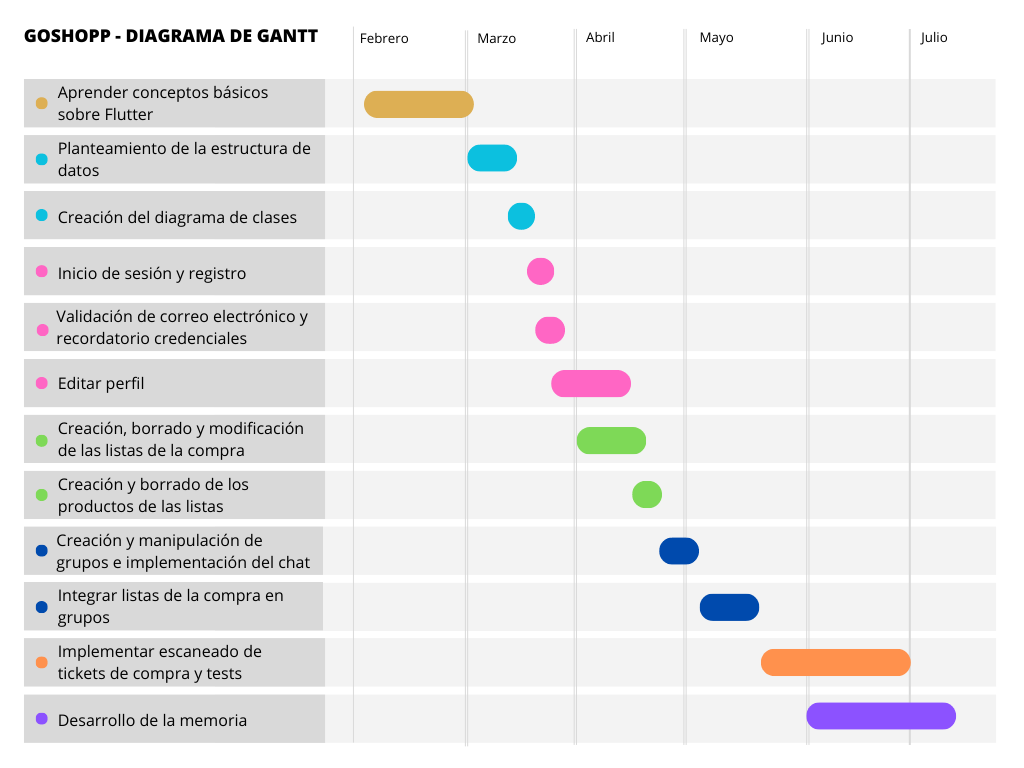
\includegraphics[width=1\textwidth]{imagenes/diagrama_gantt.png}
    \caption{Diagrama de Gantt}
\end{figure}

\subsection{Estimación económica}

Como todo proyecto, existe un coste económico muy importante, pues al final, es el que determinará si la aplicación que se está desarrollando es económica y empresarialmente viable o no, pues es obvio que no tendría sentido desarrollar una aplicación que haga perder dinero al cliente que la va a utilizar.

Se realizará una estimación bajo la suposición de que este proyecto se desarrollase bajo la contratación de una única persona con los conocimientos técnicos correspondientes para tal fin, es decir, un programador, en este caso junior. Para ello, se han utilizado datos obtenidos de páginas como Indeed, Glassdoor, Jobted o Hack a Boss, cuyo objetivo se basa en proporcionar recursos y facilitar la búsqueda de empleo, así como obtener información acerca del mismo.

Basándose en esto, se debe tener en cuenta que el sueldo medio oscila entre 18.000 y 24.000 euros brutos anuales, lo que se correspondería con unos entre 10 y 14 euros brutos por hora de trabajo. Dado que se le ha dedicado al proyecto unas tres o cuatro horas diarias, cuatro días a la semana, durante prácticamente cuatro meses, el trabajo del programador estaría rondando entre 3200 y 4400 euros brutos. Para este caso, se pondrá una cantidad media de 3800 euros.

Sin embargo, no solo se debe tener en cuenta el coste económico del trabajo del personal, sino también el coste del material inventariable utilizado. En este caso, se ha utilizado un ordenador personal HP Pavilion 15s, con 12 GB de memoria RAM DDR4, 1 TB de disco duro SSD y un procesador Intel Core i7 de décima generación valorado en aproximadamente 600 euros, y un monitor adicional iiyama Prolite de 23.8" Full HD, valorado en 290 euros. Disponer este monitor adicional ha ayudado a agilizar en gran medida el desarrollo del proyecto.

A todo ello, se debe sumar el coste de publicar la aplicación en las tiendas oficiales correspondientes de los distintos sistemas operativos. Para ello, se tienen dos principales opciones:

\begin{enumerate}
    \item Publicar la aplicación en Google Play para usuarios de Android, para lo cual sería necesario subsanar un pago único de unos 32 euros.
    \item Publicar la aplicación en el AppStore para que sea accesible mediante dispositivos iOS, lo que requiere una cuota de inscripción anual de unos 92 euros por acceder al Programa de Desarrolladores de Apple y poder publicar en dicha tienda.
\end{enumerate}

Todo esto conllevaría un coste total del proyecto de unos 5000 euros más los gastos de publicación en tiendas oficiales, sin contar los gastos que debe subsanar una empresa entre impuestos, seguridad social, etc.

\section{Marco teórico}

\subsection{Antecedentes teóricos}

Una aplicación móvil es un software diseñado específicamente para ser utilizado en dispositivos móviles, como teléfonos inteligentes y tabletas. Estas aplicaciones se instalan en el dispositivo del usuario y ofrecen una amplia gama de funciones y servicios, que van desde la comunicación y el entretenimiento hasta la productividad y la gestión de tareas. Las aplicaciones móviles pueden ser descargadas e instaladas desde las tiendas de aplicaciones correspondientes a cada plataforma móvil, como Google Play Store para dispositivos Android o App Store para dispositivos iOS.

La importancia de las aplicaciones móviles en la actualidad es innegable debido al creciente uso de dispositivos móviles en todo el mundo. Estas aplicaciones se han convertido en una parte integral de la vida cotidiana de las personas, facilitando la realización de diversas tareas y brindando acceso a una amplia gama de servicios con solo unos pocos toques en la pantalla. Permiten a los usuarios acceder a información en tiempo real, comunicarse de manera efectiva, realizar compras en línea, acceder a servicios bancarios, jugar, hacer ejercicio e incluso trabajar, entre muchas otras actividades.

En consecuencia con esto, a lo largo de los años la forma en que las personas han anotado sus listas de la compra ha evolucionado significativamente. Desde los métodos tradicionales hasta las soluciones digitales más modernas, el proceso de hacer una lista de la compra ha experimentado cambios en respuesta a la tecnología y a las necesidades de los consumidores.

En tiempos pasados, e incluso en algunos casos a día de hoy, las listas de la compra se solían escribir a mano en papel. Este método clásico implicaba tomar un bolígrafo y anotar manualmente los artículos necesarios en una hoja de papel. Estas listas solían perderse con facilidad o resultar inaccesibles cuando se necesitaban en el momento de hacer las compras, además de necesitar de un previo consenso con todos los integrantes del grupo familiar o de amigos para asegurarse de que no faltaba ni sobraba nada de lo anotado.

Con el advenimiento de las tecnologías electrónicas, surgieron nuevas formas de gestionar las listas de la compra. Una de ellas fue el uso de aplicaciones de procesamiento de texto o blocs de notas en los dispositivos personales de cada persona, lo que permitía editar y guardar fácilmente la lista en formato digital. Sin embargo, esta opción seguía haciendo algo complejo el mantenimiento de varias listas a la vez, además de seguir necesitando de una comunicación con el resto de personas para asegurarse de que la compra se realizaba correctamente.

\newpage
Con el avance de los dispositivos móviles, como los teléfonos inteligentes y las tabletas, se abrió un nuevo mundo de posibilidades para la gestión de las listas de la compra. Surgieron aplicaciones móviles dedicadas específicamente a esta tarea. Estas aplicaciones permiten a los usuarios crear y administrar fácilmente sus listas de la compra directamente en sus dispositivos. Proporcionan características prácticas, como la capacidad de agregar artículos rápidamente, organizar la lista por categorías, establecer recordatorios y sincronizarla con otros dispositivos.

En la actualidad, también han surgido soluciones más avanzadas basadas en la inteligencia artificial y el reconocimiento de voz. Estas aplicaciones permiten a los usuarios dictar su lista de la compra en lugar de escribirla o incluso crear automáticamente listas basadas en patrones de compra anteriores.

\subsection{Aplicaciones similares}

La creación de una aplicación móvil implica una cuidadosa consideración de las aplicaciones existentes en el mercado que pueden ser similares en términos de funcionalidad o propósito. Estas aplicaciones similares pueden ofrecer características y servicios relacionados que podrían competir o complementar la aplicación móvil desarrollada. Por lo tanto, es esencial realizar un análisis exhaustivo de las aplicaciones comparables como parte del proceso de investigación y desarrollo.

En el ámbito de las aplicaciones móviles para la gestión de listas de la compra, existen diversas alternativas que han ganado popularidad y se han posicionado en el mercado. Es importante destacar que cada aplicación tiene sus propias fortalezas y debilidades, y puede dirigirse a diferentes segmentos de usuarios o brindar una experiencia única. Por lo tanto, al introducir una nueva aplicación móvil en el mercado, es fundamental destacar los aspectos distintivos y ventajas competitivas que ofrece, ya sea en términos de funcionalidad, usabilidad, diseño de interfaz de usuario o características innovadoras.

A continuación, se detallarán algunas de las principales aplicaciones móviles que abarcan el mercado que nos concierne, destacando sus ventajas, inconvenientes y aspectos interesantes que se han tomado como ejemplo para la aplicación que se ha desarrollado.

\subsubsection{Bring!}

Una de las características distintivas de \textit{Bring!} es su interfaz intuitiva y fácil de usar. Al abrir la aplicación, los usuarios pueden crear nuevas listas de la compra y personalizarlas según sus necesidades. La aplicación ofrece una amplia variedad de categorías predefinidas, como alimentos, productos de limpieza, artículos de baño, entre otros, lo que facilita la organización de los elementos en la lista. Ambas características son una gran ventaja, pues ofrecen al usuario un mayor número de posibilidades a la hora de utilizar la aplicación.

La funcionalidad de compartir listas es otra característica destacada de \textit{Bring!}. Los usuarios pueden compartir sus listas con familiares, compañeros de cuarto o amigos, permitiendo una colaboración eficiente en la planificación de las compras. Esto es especialmente útil cuando varios usuarios comparten responsabilidades o necesitan coordinarse en la adquisición de productos.

Además de estas funcionalidades, \textit{Bring!} se destaca por su integración con tiendas en línea. La aplicación permite a los usuarios buscar y comprar directamente los elementos de la lista a través de socios minoristas seleccionados, ofreciendo una experiencia de compra fluida y conveniente.

\subsubsection{Listonic}

\textit{Listonic} es una aplicación móvil popular y ampliamente utilizada para gestionar listas de la compra de manera eficiente y práctica. Esta aplicación está diseñada para ofrecer una experiencia sencilla y conveniente a los usuarios al crear y administrar sus listas de la compra. Al igual que todas las demás, también ofrece la posibilidad de categorizar los elementos de la lista según diferentes categorías, como lácteos, frutas, carnes, etc., así como compartir las listas de la compra con otros usuarios.

Una de las características destacadas de \textit{Listonic} es su capacidad de reconocer automáticamente los productos mientras se escriben en la lista. Esto facilita y agiliza el proceso de añadir elementos, ya que la aplicación sugiere opciones a medida que se va escribiendo.

La aplicación ofrece también la posibilidad de establecer recordatorios para las compras. Los usuarios pueden configurar alertas basadas en fechas y horas específicas, asegurándose de no olvidar ningún elemento de la lista durante sus visitas al supermercado.

\subsubsection{HNGRY}

Al igual que las dos anteriores, se trata de una aplicación móvil utilizada para gestionar listas de la compra, con la diferencia de que está más reciente. Esto hace que tenga menos popularidad que el resto pero, sin embargo, cuenta con una serie de funcionalidades innovadoras respecto a las otras dos.

Entre estas funcionalidades innovadoras destaca su sistema de inteligencia artificial y de aprendizaje automático, el cual sugiere los artículos que faltan en la lista de la compra en función a los ya añadidos o de compras anteriores. Sin embargo, estas funciones están limitadas en su versión gratuita, por lo que para disfrutar al completo de todas las funcionalidades que ofrece se tendría que abonar una suscripción mensual.

\subsection{Diferenciación de la competencia}

A recomendación del tutor y basándome en algunas funcionalidades avanzadas de inteligencia artificial ya comentadas, surgió la idea de implementar una función de escaneo de tickets, ya que ninguna de las principales aplicaciones en el sector lo tienen. Si bien es cierto que algunas aplicaciones permiten escanear códigos de barras para obtener los productos, un escaneo del ticket completo se entiende como una funcionalidad mucho más completa y útil, pues evita la introducción manual de los productos comprados uno a uno.

Además, como se ha podido comprobar, todas las aplicaciones presentadas necesitan de otra red social o aplicación de mensajería externas para poder compartir las listas creadas con otros usuarios o comunicarse con ellos. Con \textit{GoShopp} y su funcionalidad de chat de grupo, este problema está resuelto, pudiendo establecer una comunicación fluida con el resto de integrantes del grupo sin salir de la aplicación.

\section{Descripción de las tecnologías utilizadas}

A continuación se presentarán las herramientas y tecnologías que han sido utilizadas en el desarrollo del proyecto, las cuales ha sido seleccionadas cuidadosamente para asegurar la eficiencia, funcionalidad y escalabilidad del sistema, con el objetivo de crear una solución robusta y adaptada a las necesidades del proyecto.

\subsection{Flutter}

\begin{figure}[h]
    \centering
    
\includegraphics[width=0.2\textwidth]{imagenes/logos/logo_flutter.png}
\end{figure}

La aplicación ha sido desarrollada utilizando Flutter \cite{Flutter}, un marco de código abierto desarrollado y compatible con Google. Es ampliamente utilizado por desarrolladores de front-end o fullstack para crear interfaces de usuario para varias plataformas con un único código base.

Cuando se lanzó Flutter en 2018, se centraba principalmente en el desarrollo de aplicaciones móviles. En la actualidad, además del desarrollo de aplicaciones para iOS y Android, Flutter también es compatible con aplicaciones web, Windows, MacOS y Linux.

En cuanto al uso de Flutter en el desarrollo de aplicaciones multiplataforma, se pueden encontrar varias ventajas \cite{Flutter 1}:

\begin{enumerate}
    \item Flutter utiliza el lenguaje de programación Dart, del cual se hablará más adelante. Dart se compila en código máquina, que es entendido por los dispositivos host, lo que garantiza un rendimiento rápido y eficiente, comparable al rendimiento ofrecido por otros marcos de programación de aplicaciones nativas, como Android Studio (para Android) o Xcode (para iOS).
    \item En lugar de depender de herramientas de renderización específicas de la plataforma, Flutter utiliza la biblioteca gráfica de código abierto \textit{Skia} de Google para renderizar la interfaz de usuario. Esto proporciona una apariencia visual consistente a los usuarios, independientemente de la plataforma que utilicen para acceder a una aplicación.
    \item Flutter cuenta con herramientas como la recarga en caliente, que permite a los desarrolladores previsualizar los cambios en el código sin perder el estado de la aplicación, y el inspector de widgets, que facilita la visualización y resolución de problemas en los diseños de la interfaz de usuario.
\end{enumerate}

Como se mencionó anteriormente, el lenguaje de programación utilizado por Flutter es Dart \cite{Dart}, que también es desarrollado por Google y es de código abierto. En sus inicios, se presentó como un \textit{lenguaje estructurado pero flexible para programación web} en la conferencia de presentación en 2011. Sin embargo, debido a la evolución de Flutter en el desarrollo de aplicaciones multiplataforma, Dart ha ganado relevancia en el mundo del desarrollo de software para dispositivos móviles.

Dart se destaca por ser un lenguaje de programación de alto nivel y orientado a objetos, diseñado para ser fácil de aprender y ofrece una sintaxis clara y concisa. También utiliza un enfoque de compilación anticipada, lo que significa que el código fuente se compila en código nativo antes de su ejecución, lo que permite una ejecución rápida y eficiente. Además, tiene la capacidad de ejecutarse tanto en el lado del cliente como en el lado del servidor.

La curva de aprendizaje de lenguajes como Dart y, sobre todo, de entornos como Flutter, puede ser muy vertical, especialmente si no se tiene experiencia previa. Por ello, en un inicio, se dedicaron bastantes días e incluso semanas al aprendizaje en profundidad acerca de dicho lenguaje, ya fuese mirando tutoriales sobre el mismo, leyendo la documentación oficial acerca de los widgets que ofrece e, incluso, creando algunas aplicaciones básicas para ir probando su comportamiento, antes de pasar a un proyecto de mayor envergadura como este.

La aplicación de contador de clicks es un ejemplo común que se utiliza en muchos tutoriales y guías introductorias para Flutter. Tanto es así, que siempre que se crea un nuevo proyecto en Flutter, el entorno nos proporciona este código por defecto. Es una aplicación simple que permite contar y mostrar la cantidad de veces que se ha hecho clic en un botón, lo que permite fácilmente aprender el funcionamiento de los widgets y como estos interactúan con la aplicación.

\subsection{Visual Studio Code}

\begin{figure}[h]
    \centering
    
\includegraphics[width=0.25\textwidth]{imagenes/logos/logo_vscode.png}
\end{figure}

El editor de código fuente utilizado ha sido Visual Studio Code \cite{VSCode}, un IDE ligero pero potente disponible para Windows, macOS y Linux. Una de sus principales fortalezas es su soporte integrado para una amplia gama de lenguajes de programación. Viene con resaltado de sintaxis, autocompletado inteligente y sugerencias de código, lo que facilita la escritura y comprensión del código. Además, cuenta con herramientas de depuración y control de versiones, lo que permite a los desarrolladores solucionar errores y colaborar en proyectos de manera más eficiente.

Otra ventaja significativa de Visual Studio Code es su extensibilidad. El editor cuenta con un rico ecosistema de extensiones que permiten ampliar sus funcionalidades para adaptarse a diferentes lenguajes y entornos de programación. Estas extensiones abarcan desde temas personalizados y mejoras de productividad hasta integraciones con herramientas y servicios externos. Esto nos ofrece la posibilidad de personalizar nuestro entorno de desarrollo de acuerdo a nuestras necesidades específicas.

En el contexto del desarrollo de aplicaciones Flutter, Visual Studio Code ofrece una integración completa con este framework multiplataforma, puediendo así aprovechar las extensiones específicas de Flutter que proporcionan características adicionales para agilizar el proceso de desarrollo. Esto incluye la capacidad de editar, corregir, compilar y ejecutar el código en tiempo real, utilizando un emulador previamente instalado en el dispositivo. Esta integración garantiza una experiencia de desarrollo rápida y eficiente, ya que los cambios realizados se reflejan instantáneamente en el contenido del emulador con solo guardar los cambios en el código.

\subsection{Android Studio}

\begin{figure}[h]
    \centering
    
\includegraphics[width=0.25\textwidth]{imagenes/logos/logo_androidstudio.png}
\end{figure}

\vspace{0.3cm}

Al igual que Visual Studio Code, Android Studio \cite{Android Studio} es un entorno de desarrollo integrado exclusivo para el desarrollo de aplicaciones enfocadas en el sistema operativo de Android. Desarrollado por Google, Android Studio es una herramienta ampliamente utilizada que ofrece una serie de características y funcionalidades específicas para facilitar el desarrollo de aplicaciones Android.

En este proyecto en particular, Android Studio ha sido utilizado para aprovechar el rendimiento de sus emuladores. Dichos emuladores permiten simular dispositivos Android en el entorno de desarrollo, lo que resulta especialmente útil durante el proceso de desarrollo y pruebas. Con solo seleccionar la opción deseada y esperar una breve descarga, es posible crear un emulador que se ajuste a las necesidades del proyecto.

En este caso, se ha utilizado el emulador Pixel 6 Pro API 33, conocido por ofrecer un excelente rendimiento y aprovechar al máximo las capacidades del dispositivo de desarrollo. Además, es posible personalizar diversas características, como la cantidad de RAM y otras especificaciones, lo que permite simular diferentes escenarios y condiciones para probar el rendimiento de la aplicación en una variedad de situaciones. También ofrece compatibilidad con las últimas versiones de Android y las características más recientes del sistema operativo, lo que permite aprovechar las últimas innovaciones y funcionalidades disponibles.

Además, y como se ha explicado anteriormente, esta integración con Android Studio ha permitido editar el código de la aplicación en Visual Studio Code, utilizando el lenguaje de programación Dart en el entorno de Flutter. Desde la propia ventana de Visual Studio Code, simplemente abriendo el emulador y ejecutando la aplicación, es posible visualizar el resultado en tiempo real en uno de estos emuladores.

Finalmente, se destaca la capacidad de recargar el contenido del emulador rápidamente con solo guardar los cambios realizados en el editor de código. Esta sincronización fluida entre Android Studio, Visual Studio Code y los emuladores facilita significativamente el proceso de desarrollo, ya que cualquier modificación realizada se refleja instantáneamente en la aplicación emulada, agilizando así las pruebas y la iteración en el desarrollo de la aplicación Android.

\subsection{Firebase}

\begin{figure}[h]
    \centering
    
\includegraphics[width=0.3\textwidth]{imagenes/logos/logo_firebase.png}
\end{figure}

Firebase \cite{Firebase} es una plataforma digital alojada en la nube diseñada para facilitar el desarrollo de aplicaciones web y móviles de calidad de forma rápida y eficiente. Su objetivo es mejorar el rendimiento de las aplicaciones a través de la implementación de sus distintos módulos, que hacen que la aplicación sea más manejable, segura y fácil de utilizar para los usuarios.

En 2014, después de experimentar un gran crecimiento, Google adquirió Firebase, lo que brinda a las aplicaciones un soporte de calidad. Además, Firebase ofrece sus propios servidores en la nube para almacenar bases de datos, lo que es especialmente beneficioso. En gran medida, esta plataforma es gratuita, lo cual es una de las razones principales por las que se elige esta herramienta. Otra razón es la amplia gama de módulos que ofrece, que son totalmente compatibles con Flutter. A continuación, se describen algunos de ellos:

\begin{enumerate}
    \item \underline{Firebase Authentication} \cite{Firebase 1}: Permite la autenticación de usuarios mediante diversos mecanismos, como correo electrónico y contraseña, teléfono móvil o aplicaciones externas como Google, Twitter y Facebook. En este caso, se permite la autenticación mediante correo electrónico y contraseña, así como mediante una cuenta de Google.
    \item \underline{Firebase Cloud Storage} \cite{Firebase 2}: Es un servicio de almacenamiento de contenido potente y seguro. Además, permite escalar automáticamente el almacenamiento en función de las necesidades de la aplicación, en su mayoría de manera gratuita. Se ha utilizado para guardar información como las imágenes de perfil de los usuarios, que se recuperan mediante una URL y se almacenan en Firebase Authentication.
    \item \underline{Firebase Cloud Firestore} \cite{Firebase 3}: Es un servicio de base de datos flexible, escalable y en la nube, diseñado para almacenar y sincronizar datos en tiempo real. Los datos se estructuran como documentos organizados en colecciones.
\end{enumerate}

Además, Firebase cuenta con una generosa capa gratuita que permite a los desarrolladores comenzar a utilizar la plataforma sin incurrir en costos significativos. A medida que la aplicación crece y requiere más recursos, Firebase ofrece opciones de facturación flexibles y escalables para adaptarse a las necesidades cambiantes de la aplicación.

\subsection{Github}

GitHub es una plataforma muy popular utilizada por desarrolladores de todo el mundo para alojar y colaborar en proyectos de desarrollo de software. Proporciona un entorno basado en la nube para el control de versiones utilizando Git, un sistema de control de versiones distribuido ampliamente utilizado en la industria del desarrollo de software.

Una de las principales características de GitHub es su capacidad para trabajar con ramas y realizar 'pull requests'. Las ramas permiten a los desarrolladores crear versiones separadas de un proyecto y realizar cambios en paralelo sin afectar la rama principal o la versión estable del software. Esto facilita la colaboración entre equipos y la implementación de nuevas funcionalidades o correcciones de errores de manera controlada.

Además del control de versiones y la colaboración, GitHub también ofrece otras características útiles para organizar y administrar proyectos. Por ejemplo, los 'issues' pueden ser utilizados para rastrear problemas o errores, así como listar las tareas específicas en un proyecto. Esto ayuda a mantener un registro ordenado de los problemas identificados y su estado de resolución.

El repositorio con el código fuente del proyecto \cite{repo} se encuentra disponible para consulta de todo aquel que lo desee. 

\begin{figure}[h]
    \centering
    
\includegraphics[width=0.2\textwidth]{imagenes/logos/logo_github.png}
\end{figure}

\subsection{ProtoPie}

ProtoPie es una aplicación que se utiliza para crear prototipos de interfaces de aplicaciones, siendo compatible tanto con dispositivos de escritorio como con dispositivos móviles. Su principal función es facilitar el diseño de bocetos de la interfaz y prototipos interactivos del funcionamiento de la aplicación. Sin embargo, en el contexto de este proyecto en particular, no se requirió utilizar los prototipos interactivos, ya que se tenía una clara comprensión de la experiencia de usuario desde el inicio.

A pesar de esto, ProtoPie fue una herramienta muy útil para crear los bocetos de las diversas pantallas del software. Estos bocetos fueron posteriormente implementados en Flutter utilizando los widgets proporcionados por la plataforma.

A continuación, se presentan los modelos creados para las diferentes pantallas de la aplicación. Es importante destacar que en el resultado final se incluyen otras pantallas que se describirán más adelante. Estas pantallas adicionales no requirieron modelos debido a su simplicidad.

\begin{figure}[h]
    \centering
    
\includegraphics[width=0.3\textwidth]{imagenes/logos/logo_protopie.png}
\end{figure}

\begin{figure}[htbp]
    \centering
    \begin{subfigure}[h]{0.3\textwidth}
        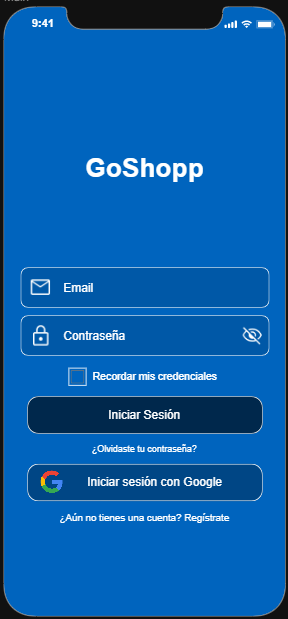
\includegraphics[width=\textwidth]{imagenes/modelos/login.png}
    \end{subfigure}
    \hfill
    \begin{subfigure}[h]{0.3\textwidth}
        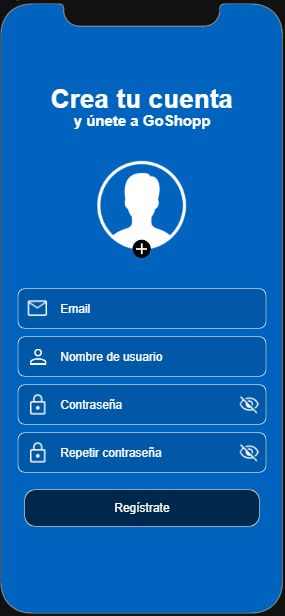
\includegraphics[width=\textwidth]{imagenes/modelos/registro.png}
    \end{subfigure}
    \hfill
    \begin{subfigure}[h]{0.3\textwidth}
        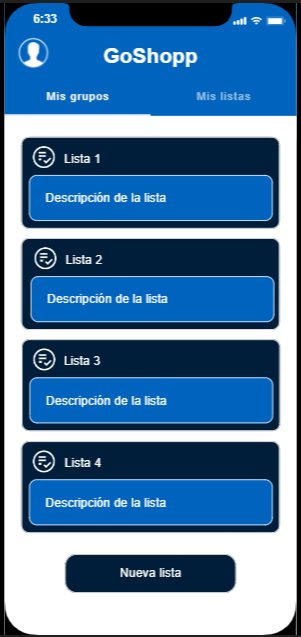
\includegraphics[width=\textwidth]{imagenes/modelos/listas.png}
    \end{subfigure}

    \vspace{1cm}
    
    \begin{subfigure}[h]{0.3\textwidth}
        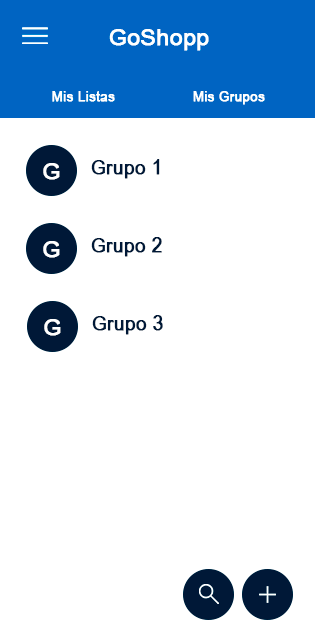
\includegraphics[width=\textwidth]{imagenes/modelos/grupos.png}
    \end{subfigure}
    \hfill
    \begin{subfigure}[h]{0.3\textwidth}
        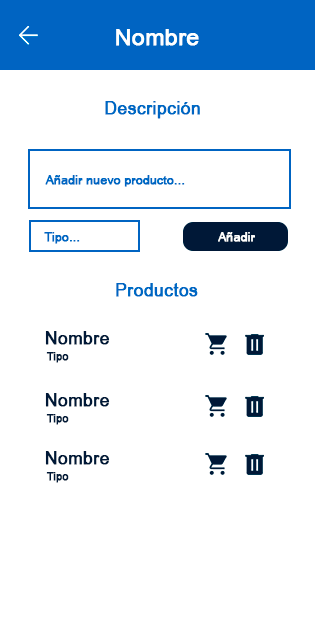
\includegraphics[width=\textwidth]{imagenes/modelos/detalles.png}
    \end{subfigure}
    \hfill
    \begin{subfigure}[h]{0.3\textwidth}
        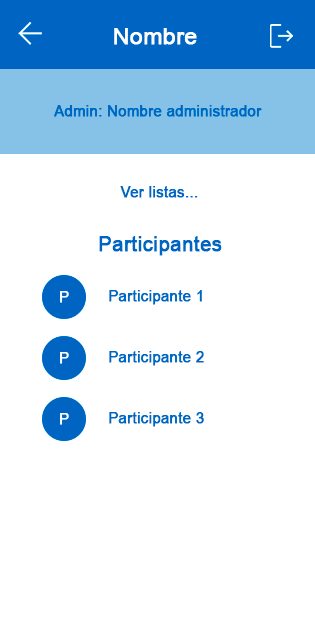
\includegraphics[width=\textwidth]{imagenes/modelos/info.png}
    \end{subfigure}
    
    \caption{Primeros prototipos de las distintas pantallas de la aplicación}
\end{figure}

\section{Arquitectura interna}

\subsection{Autenticación de usuarios}

Para explicar el sistema de autenticación de usuarios, se debe basar, como se mencionó anteriormente, en el funcionamiento del módulo Firebase Auth \cite{Firebase Authentication}, que permite autenticar usuarios en la aplicación tanto mediante el uso de correo electrónico y contraseña, como mediante aplicaciones externas como Google, Facebook, etc.

Lo más común en todas las aplicaciones existentes es el primero de los casos mencionados. Para ello, es necesario realizar una serie de validaciones, como verificar que el correo electrónico tenga un formato válido o que ninguno de los campos, excepto el de imagen, se encuentren vacíos. Si alguna de las validaciones que se van a comentar a continuación falla, el usuario recibirá una notificación flotante de color rojo en la que podrá obtener información de dicho error. En el caso que todas las comprobaciones se pasen con éxito, se creará el usuario en nuestro sistema y el usuario será informado de la misma forma que con los errores, pero esta vez con el mensaje en color verde, para hacerlo más intuitivo a primera vista.

La primera comprobación que se realiza, lo único que se debe verificar es que los distintos controladores de los campos de texto no se encuentren vacíos, de la siguiente forma:

\vspace{0.5cm}
\begin{codigo}
if (_usuarioController.text.isEmpty || 
    _emailController.text.isEmpty ||
    _contrasenaController1.text.isEmpty ||
    _contrasenaController2.text.isEmpty)
{
    mostrarSnackBar("Debe rellenar todos los campos.", "error", context);
}
\end{codigo}

Tras esto, se pasa a la siguiente comprobación, de manera vertical descendente, por lo que se procede a la validación del formato del correo electrónico introducido. Para ello, se ha utilizado un paquete de Flutter llamado \textit{email\_validator} \cite{Email Validator}, que contiene una función que, al ser llamada con un parámetro de tipo String, devuelve un valor booleano dependiendo de si el formato es el de un correo electrónico o no. Entiéndase por formato de correo electrónico aquel formado por una cadena de caracteres, seguida de un @ obligatorio, tras el cual aparecerá un dominio, es decir, dos cadenas separadas por un punto y, opcionalmente, otra cadena precedida de otro punto, como puede ser el caso, por ejemplo, del correo académico de un estudiante de la Universidad de Granada (\textit{ejemplo@ugr.es} o \textit{ejemplo@correo.ugr.es}):

\vspace{0.5cm}
\begin{codigo}
else if (!EmailValidator.validate(_emailController.text))
{
    mostrarSnackBar('El correo introducido no tiene un formato correcto.',
    "error", context);
}
\end{codigo}

Posteriormente, también se han realizado validaciones para la contraseña, por motivos de seguridad, por lo que deberán tener al menos 6 caracteres. También en un futuro y como mejora se podrían añadir más validaciones de seguridad, como la obligatoriedad de alguna mayúscula o de caracteres especiales pero, como se mencionará en el último apartado de este documento, el objetivo es acabar con el uso de contraseñas debido a su vulnerabilidad.

También, y como última validación, se comprobará que ambas contraseñas coincidan. Esto, junto al botón de visualizar u ocultar contraseña situado en el propio campo del formulario, permitirá al usuario asegurarse al máximo de que la contraseña introducida es la que realmente desea.

\begin{codigo}
else if (_contrasenaController1.text.length < 6)
{
    mostrarSnackBar('La contrasena debe tener al menos 6 caracteres.',
    "error", context);
}
else if (_contrasenaController1.text != _contrasenaController2.text)
{
    mostrarSnackBar('Las contrasenas no coinciden.', "error", context);
}
\end{codigo}

Finalmente, y para acabar las validaciones de registro de usuarios, se debe comprobar que el correo electrónico introducido por el usuario no existe ya en nuestra base de datos, para lo cual, a la hora de registrar al usuario usando Firebase Auth, se obtiene el error como una excepción específica de Firebase. De esta forma, se pueden detectar los distintos errores que se pueden producir:

\vspace{0.5cm}
\begin{codigo}
try {
    // Se registra al usuario en la base de datos
} on FirebaseAuthException catch (e)
{
    if (e.code == "email-already-in-use")
    {
        mostrarSnackBar("Ya existe un usuario con ese correo electronico.",
        "error", context);
    } else
    {
        mostrarSnackBar("Lo sentimos, hubo un error", "error", context);
    }
}
\end{codigo}

En cuanto al inicio de sesión de los usuarios, la única validación que se hace en cuanto al formulario, al igual que en el registro, es que los campos del formulario, tanto el correo electrónico como la contraseña, no estén vacíos. Seguidamente, cuando se inicia sesión, se pueden obtener dos tipos de errores mediante Firebase:

\vspace{0.5cm}
\begin{codigo}
try {
    // Se realiza el inicio de sesion
} on FirebaseAuthException catch (e) {
    if (e.code == "user-not-found" || e.code == "wrong-password")
    {
      mostrarSnackBar("Los valores introducidos no son correctos.", "error",
      context);
    }
    else
    {
      mostrarSnackBar("Asegurese de rellenar todos los campos.", "error",
      context);
    }
}
\end{codigo}

Además, se ha permitido iniciar sesión con una cuenta de Google existente, utilizando un paquete llamado \textit{google\_sign\_in} \cite{Google Sign In}, que permite autenticarse en la aplicación seleccionando una cuenta de Google ya almacenada en el sistema. En el caso de que sea la primera vez que el usuario usa esta opción, se creará la cuenta en la base de datos. Si, por el contrario, el usuario ya inició sesión con su cuenta de Google en otro momento, simplemente se realizará un inicio de sesión normal.

Finalmente, como funcionalidad adicional, se ha habilitado la opción de guardar las credenciales. Si se marca la casilla correspondiente, al cerrar la aplicación se guardarán los datos introducidos en los cuadros de texto y, al volver a abrirla, aparecerán ya rellenos. En caso de no marcarla, los campos aparecerán vacíos. Para lograr esto, se utiliza otro módulo de Flutter llamado \textit{shared\_preferences} \cite{Shared Preferences}.

Es posible acceder a la consola de Firebase para controlar el proyecto. En la pestaña 'Authentication', se pueden ver todos los usuarios registrados, su método de inicio de sesión y su autenticador. Podemos verlo en el siguiente ejemplo, en el cual, por seguridad, se ha censurado la información sensible de los usuarios:

\begin{figure}[h]
    \centering
    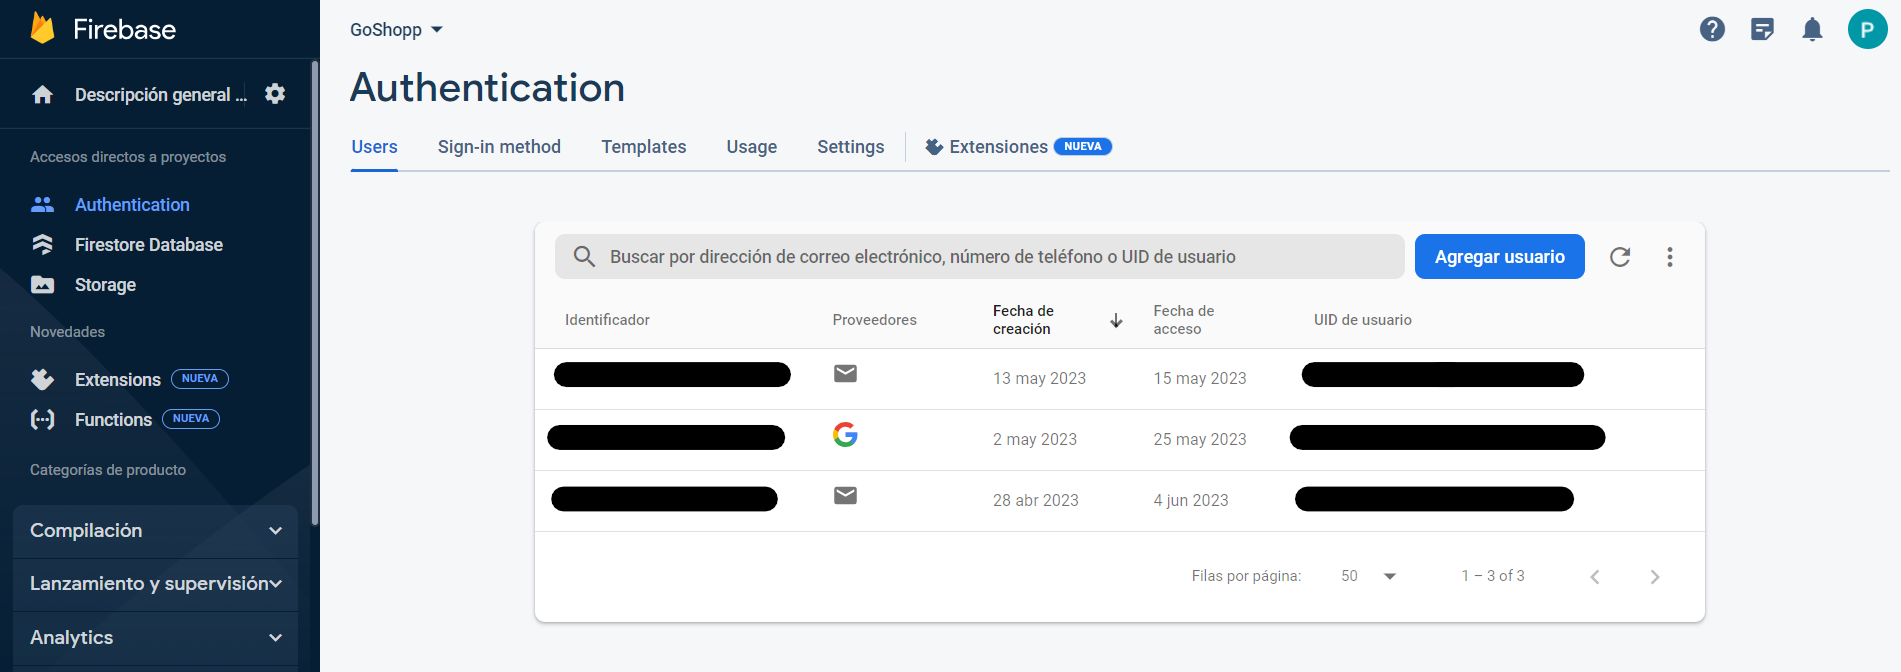
\includegraphics[width=1\textwidth]{imagenes/firebase_auth.png}
    \caption{Firebase Auth}
\end{figure}

También cabe destacar que, para guardar las imágenes de perfil de los usuarios, se ha utilizado la dependencia \textit{firebase\_storage} \cite{Firebase Storage} que permite almacenar imágenes y ficheros en la nube de Firebase ofreciéndonos, en código, un enlace para acceder a ella. A posteriori, se utiliza dicho enlace para guardar la imagen en el atributo \textit{photoURL} del tipo de dato User de Firebase y poder recuperarla en cualquier parte de nuestro código.

\subsection{Estructura de datos}

Uno de los pasos más importantes a la hora de crear una aplicación, sea del tipo que sea, es el diseño y la implementación de la estructura de datos. Para ello, lo primero que se hizo fue plantear qué clases podían ser necesarias pues, aunque parece obvio que debe haber una clase para representar las distintas listas de la compra y otra para representar sus respectivos productos, no es tan sencillo debido a los problemas que comentaré más adelante.

Finalmente, se optó por una estructura de clases formada por cinco clases y otra de tipo 'Enumeración', de manera que todas están relacionadas entre sí unas con otras. Se describen a continuación:

\begin{itemize}
    \item \underline{Enumerado TipoProducto}: representa cada uno de los tipos que puede tomar un producto de una lista, ya que no simplemente nos limitaremos a listas de la compra de supermercados, sino algo mucho más general De esta forma, podemos encontrar desde comida o bebida, hasta electrodomésticos, ropa, medicamentos, mobiliario o productos de deporte, ocio o belleza, entre otros.
    \item \underline{Clase Producto}: representa cada uno de los productos que se pueden añadir a una lista de la compra, indicando su tipo, precio, nombre y si está o no comprado.
    \item \underline{Clase ListaCompra}: representa cada una de las listas de la compra, independientemente de si es cooperativa o no, indicando su nombre, descripción, id, el id del propietario de la misma y un listado de los productos que contiene.
    \item \underline{Clase Usuario}: representa cada uno de los usuarios de la aplicación. Llegados a este punto, había un problema que resolver, y es si se debía crear una clase para almacenar los usuarios o, por el contrario, mantener únicamente la clase User que viene incluida en el paquete Firebase Authentication. Finalmente, acabó tomando más fuerza la primera opción, pues permite añadir más información sobre los usuarios como, por ejemplo, un listado de grupos a los que pertenece o un listado de las listas de la compra personales que ha creado.
    \item \underline{Clase Grupo}: representa cada uno de los grupos que se han creado, mostrando información acerca de quién es su administrador, sus participantes y un listado tanto de mensajes que se han producido en el chat de dicho grupo, del que hablaremos más tarde, como de listas de la compra cooperativas del mismo.
    \item \underline{Clase Mensaje}: representa cada uno de los mensajes que se envían por un grupo, indicando el contenido del mismo, el usuario emisor y la hora de envío.
\end{itemize}

De esta forma, el diagrama de clases final de la aplicación queda de la siguiente manera:

\begin{figure}[h]
    \centering
    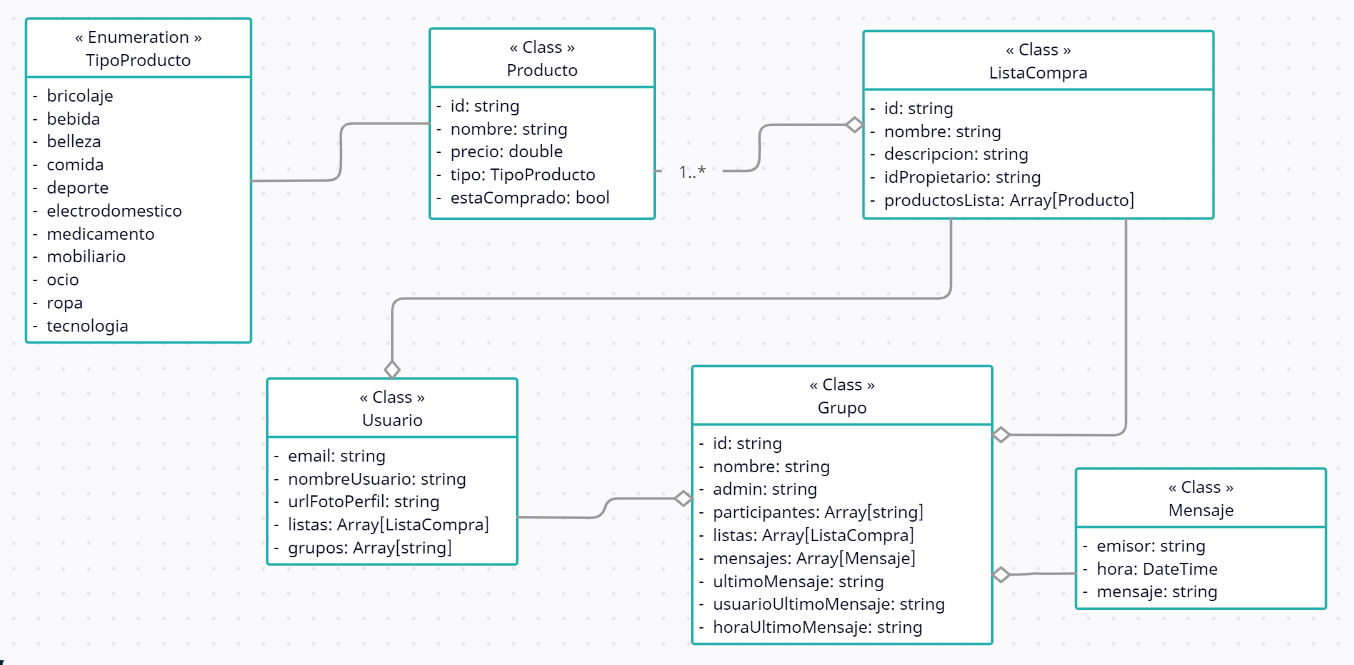
\includegraphics[width=1\textwidth]{imagenes/diagrama_clases.png}
    \caption{Diagrama de clases de la aplicación desarrollada}
\end{figure}

Uno de los problemas encontrados llegados a este punto, fue plantear las distintas posibilidades que existen en Flutter para crear bases de datos e implementar dicha estructura de datos atendiendo a las ventajas e inconvenientes de cada una de ellas. A continuación, se detallan las tres opciones que se tuvieron en cuenta, así como las ventajas e inconvenientes de usar unas u otras:

\begin{itemize}
    \item \underline{SQLite}: es una biblioteca de código abierto que se utiliza para crear y administrar bases de datos locales en las aplicaciones móviles. Permite a los desarrolladores almacenar y recuperar datos de manera eficiente, lo que resulta útil para aplicaciones que requieren un almacenamiento de datos local, como aplicaciones de chat o notas. En contrapartida, es el propio desarrollador el que debe hacerse cargo del mantenimiento de las mismas, además de tener una escalabilidad limitada, pues sufre bastante cuando hay una gran cantidad de datos y consultas. 
    \item \underline{Firebase Realtime Database}: se trata de un módulo de Firebase con una gran capacidad para mantener los datos sincronizados en tiempo real en todos los clientes, de manera que los cambios se propagan rápidamente a todos los dispositivos conectados, lo que permite una colaboración en tiempo real y una experiencia de usuario fluida. Utiliza un modelo de datos basado en un árbol JSON, lo que le aporta una mayor facilidad y velocidad, pero, como inconveniente, tiene consultas más limitadas y no admite combinación de condiciones, además de tener también una escalabilidad limitada.
    \item \underline{Firebase Cloud Firestore}: se trata también de un módulo de Firebase que se podría entender como una 'mejora' del anterior, pues está diseñado para escalar automáticamente a medida que crece el número de usuarios y la cantidad de datos, además de proporcionar un rendimiento rápido y estable incluso con grandes volúmenes de datos. Utiliza una estructura de datos jerárquica basada en colecciones y documentos, ofreciendo consultas más potentes y flexibles que permiten filtrar, ordenar y combinar condiciones.
\end{itemize}

Tras contemplar estas tres opciones, se tuvo claro que la mejor opción era usar la tercera, pues cuenta con muchas ventajas respecto a su predecesora, al ser prácticamente una actualización de la misma, y la forma en la que se almacenan los datos como colecciones aporta una gran facilidad de comprensión y de acceso a los datos mediante consultas. Además, es la opción que más facilidad aporta a la hora de integrar nuestro modelo de clases con la base de datos.

Para implementar estas consultas a la base de datos, se ha utilizado el módulo de Flutter \textit{cloud\_firestore} \cite{Firebase Cloud Firestore}, y se ha implementado un módulo llamado 'services' en el árbol de directorios de nuestro repositorio donde se guardan los ficheros que realizan las distintas consultas, inserciones y modificaciones en la base de datos para cada uno de los modelos, guardados en una carpeta llamada 'models' al mismo nivel de directorios. Por otro lado, se encuentra también el directorio 'screens' donde se encuentran todos aquellos ficheros que tienen que ver con la interfaz de usuario de la aplicación.

\subsection{Chat}

La sección de chat entre grupos es una funcionalidad sumamente importante en la aplicación, ya que permite una comunicación efectiva entre los integrantes de un grupo al momento de elaborar una lista de la compra. Como se ha mencionado anteriormente, esta característica evita la necesidad de abandonar la aplicación y recurrir a otras redes sociales para realizar consultas sobre productos faltantes, verificar si alguien ya los ha comprado o agregar nuevos elementos a la lista.

Al diseñar esta funcionalidad, se optó por guardar todos los mensajes enviados a un grupo en la base de datos correspondiente. Para lograrlo, se creó una nueva colección llamada 'mensajes' dentro de cada colección 'grupos', siguiendo el enfoque utilizado con la colección 'productos' dentro de 'listas'. De esta manera, cada mensaje cuenta con atributos que almacenan información relevante, como la fecha y hora del envío, el usuario que emite el mensaje y su contenido. La implementación de esta estructura de datos permite insertar cada mensaje en la base de datos cada vez que un usuario envía un mensaje al grupo, guardando también en la información del mismo el último mensaje, su hora de envío y su emisor, para poder trabajar más fácilmente con él en un momento dado.

Al acceder a la pantalla de chat, se recuperan todos los mensajes asociados al grupo y se muestran en orden inverso, de modo que el mensaje más reciente se muestra en la parte inferior del dispositivo. Para ello, se han tomado como ejemplo algunas aplicaciones de mensajería como WhatsApp o Telegram, que cuentan con una interfaz intuitiva que facilita la comunicación en tiempo real. Además, tomando como ejemplo esta última, se ha permitido que los usuarios que se unen a un grupo puedan visualizar todos los mensajes previos a su ingreso, lo cual les brinda la oportunidad de ponerse al día con la conversación en curso o familiarizarse con el contexto del grupo.

Finalmente, se optó por adaptar la interfaz de la funcionalidad de mensajería instantánea de nuestra aplicación a la de aplicaciones como las mencionadas anteriormente, pues se ha demostrado que son las que mejor funcionan, además de estar muy interiorizadas ya por todos los usuarios de este tipo de aplicaciones. De esta forma, se muestran a un lado los mensajes enviados por el usuario y al otro los recibidos, ambos en colores distintos, con un cuadro de texto en la parte inferior que permite la redacción del texto que se desea enviar.

\subsection{Reconocimiento de tickets de la compra}

Entrando de lleno en la funcionalidad estrella de la aplicación, se encuentra el reconocimiento de tickets de la compra. La implementación de esta funcionalidad tiene varios objetivos importantes. Uno de ellos es la automatización y conveniencia para los usuarios, al proporcionarles una forma rápida y práctica de agregar los productos comprados a una lista sin tener que realizar esta tarea manualmente. Esto se traduce en un ahorro significativo de tiempo y esfuerzo al evitar la introducción manual de datos, sobre todo en listas de la compra amplias, como puede ser la compra del mes de un grupo familiar en un supermercado.

\subsubsection{Obtención de la imagen que contiene el ticket}

Para ello, se plantean dos opciones en la forma en la que se obtiene el ticket: bien utilizando una imagen previamente guardada en la galería del dispositivo móvil, o bien obteniendo la imagen al momento desde la cámara del mismo. Para implementar ambas opciones, se ha hecho uso del paquete \textit{image\_picker} \cite{ImagePicker}, el cual permite obtener una imagen del dispositivo de ambas formas.

\vspace{0.5cm}
\begin{codigo}
try {
    final ImageSource? src = await abrirModalObtenerImagen(context);
    getTicket(src!);
} catch (e) {
    mostrarSnackBar("No se ha seleccionado ninguna imagen", "warn",
    context);
}
\end{codigo}

En este caso, cuando se pulsa el botón que activa dicha funcionalidad, se mostrará un modal el cual nos da a elegir de cual de las dos formas posibles deseamos obtener la imagen:

\begin{figure}[h]
    \centering
    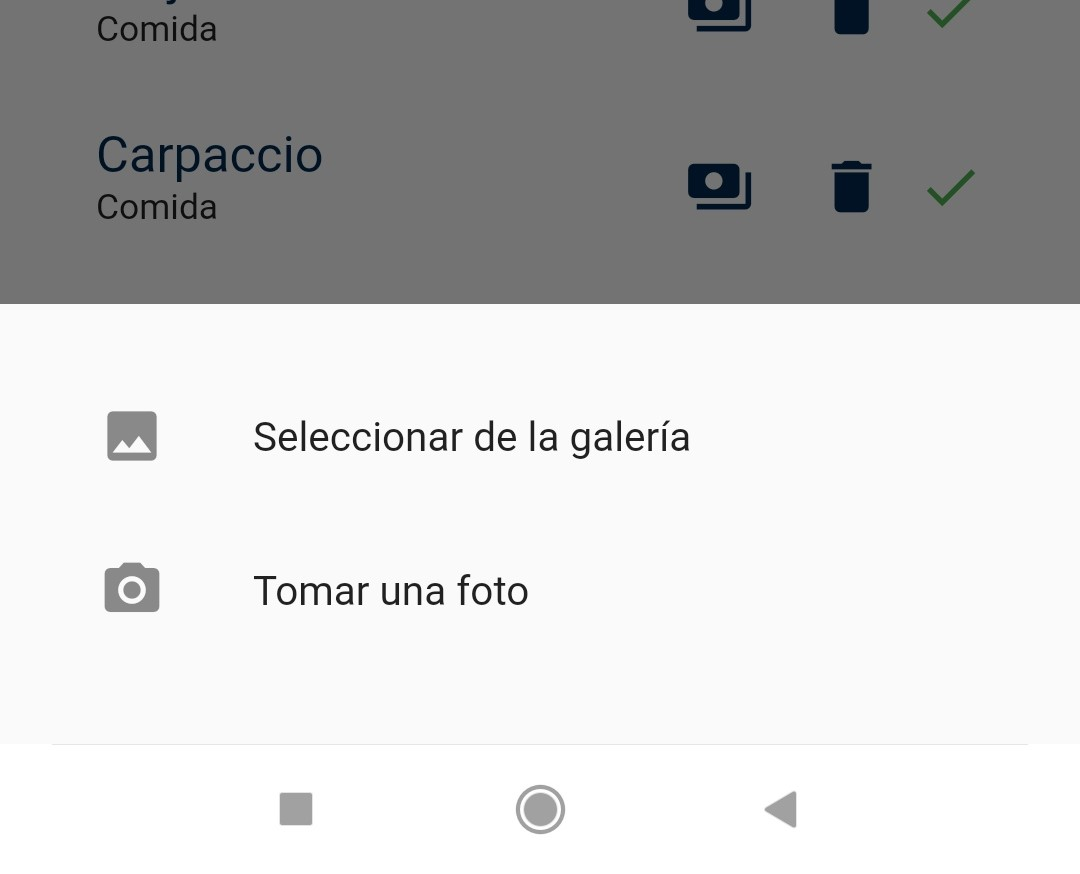
\includegraphics[width=0.55\textwidth]{imagenes/pantallas/modal_obtener_imagen.jpg}
    \caption{Seleccionar una imagen del dispositivo}
    \label{fig:modal}
\end{figure}

Una vez seleccionado el método mediante el que acceder a la imagen del ticket en cuestión, llamamos a la función \textit{getTicket} pasándole como argumento la fuente de dicha imagen, devuelta por la función \textit{abrirModalObtenerImagen}. Esta función es asíncrona para asegurarnos así de que se ha elegido o no una forma de obtener la imagen, evitando así posibles problemas de concurrencia en la ejecución del código. El contenido del ticket se obtiene de la siguiente forma:

\vspace{0.5cm}
\begin{codigo}
Future<void> getTicket(ImageSource src) async
{
    try {
        final imagenObtenida = await ImagePicker().pickImage(source: src);
        
        if (imagenObtenida == null) return;
        
        setState(() {
            this.imagen = File(imagenObtenida.path); 
        });
        
        obtenerTextoTicket(imagenObtenida);
    } catch (e) {
          mostrarSnackBar( "Se produjo un error al seleccionar la imagen",
          "error", context);
    }
}
\end{codigo}

De esta forma, se modifica la variable del widget 'imagen' con el valor de la imagen obtenida. Una vez hecho esto, se debe 'escanear' la imagen para obtener el texto de la misma. Para ello, se ha utilizado lo que se conoce como Reconocimiento Óptico de Caracteres \cite{OCR} (en inglés, OCR).

\subsubsection{Reconocimiento Óptico de Caracteres (OCR)}

El reconocimiento óptico de caracteres (OCR, por sus siglas en inglés) es una tecnología utilizada para convertir texto impreso o escrito a mano en formato digital editable. Es un proceso que implica la detección, el análisis y la interpretación de los caracteres presentes en una imagen o documento escaneado para su posterior procesamiento.

El OCR se ha vuelto ampliamente utilizado debido a su capacidad para automatizar la extracción de información de documentos físicos o digitales, lo que ahorra tiempo y esfuerzo en comparación con la transcripción manual. Utiliza algoritmos y técnicas avanzadas para reconocer y analizar los caracteres en una imagen. Esto implica el procesamiento de la imagen para mejorar el contraste y la calidad, la segmentación de los caracteres individuales y la identificación de los patrones para reconocer los caracteres específicos.

Es importante tener en cuenta que el rendimiento del OCR puede verse afectado por factores como la calidad de la imagen, el tipo y el tamaño de fuente, la legibilidad del texto y la presencia de ruido o distorsiones. Sin embargo, los avances en la tecnología han mejorado significativamente la precisión del OCR en los últimos años, lo que lo convierte en una herramienta cada vez más confiable y útil en diversas aplicaciones.

Para implementar un proceso de OCR en Flutter, se ha utilizado un paquete que llamado Google ML Kit. Se trata de un conjunto de herramientas y bibliotecas de desarrollo proporcionadas por Google que permite a los desarrolladores incorporar fácilmente la funcionalidad de aprendizaje automático en aplicaciones móviles de Android e iOS. Su objetivo es simplificar la integración de modelos de aprendizaje automático preentrenados y personalizados en aplicaciones móviles sin la necesidad de conocimientos avanzados en aprendizaje automático.

Además, ML Kit es compatible con múltiples lenguajes de programación y ofrece una API fácil de usar que permite a los desarrolladores integrar rápidamente las funciones de aprendizaje automático en sus aplicaciones, sin tener que preocuparse por detalles complejos de implementación. Para la tarea que nos incumbe, se ha utilizado una funcionalidad en concreto, llamada Text Recognition \cite{Google ML Kit}, que, como su propio nombre indica, permite reconocer y extraer texto impreso en imágenes o en tiempo real, utilizando la cámara del dispositivo.

Puede ser utilizado en diversas aplicaciones, como aplicaciones de traducción, escaneo de documentos, reconocimiento de tarjetas de visita, captura de códigos QR y muchas otras aplicaciones que requieren extraer información de texto de imágenes. Para ello, bastan con indicarle la imagen a partir de la cual queremos obtener el texto y nos devolverá una variable de tipo cadena de caracteres con todo el texto obtenido de dicha imagen de la siguiente manera:

\vspace{0.5cm}
\begin{codigo}
final input = InputImage.fromFilePath(imagen.path);
await textRecognizer.processImage(input).then((detectorTexto) {
    setState(() {
        textoObtenido = detectorTexto.text.split('\n');
        filtrarTextoObtenido();
    });
});
\end{codigo}

\subsubsection{Tratamiento del texto obtenido en el reconocimiento del ticket}

Una vez pasada la imagen obtenida anteriormente por la funcionalidad de este paquete, se obtiene una cadena de texto que contendrá toda la información del ticket: el nombre y la ubicación del supermercado, el listado de productos comprados, su precio, los impuestos aplicados y hasta el cajero que atendió la compra. Todo esto se visualizará respetando el formato vertical que caracteriza a estos documentos, por lo que podemos entender que cada línea en el ticket se corresponderá con un salto de línea en la cadena de texto obtenida. Por tanto, lo que se ha hecho es utilizar la función \textit{split} que nos rompe una cadena de texto guardándola en un vector de String conformado por aquellas partes de la cadena que están separadas, en este caso, por un salto de línea.

A continuación, lo ha se ha hecho ha sido filtrar esta cadena de texto de manera que únicamente se queden los datos que son de interés, es decir, los productos comprados. Para ello, se trabaja sobre el vector de cadenas de texto que contiene cada una de las líneas del ticket utilizando una expresión regular que se queda, únicamente, con aquellos elementos del vector que comiencen por el patrón de un número (la cantidad comprada de dicho producto), uno o varios espacios en blanco y una cadena de texto (en este caso, el nombre del producto comprado):

\vspace{0.5cm}
\begin{codigo}
filtrarTextoObtenido()
{
    RegExp regex = RegExp(r'^\s*\d{1,3}\s+.+');
    textoObtenido.removeWhere((element) => !regex.hasMatch(element));
    
    if (textoObtenido.isNotEmpty)
    {
      textoObtenido = textoObtenido
          .map((elemento) => elemento.replaceAll(RegExp(r'^\d+\s+'), ''))
          .toList();
    }
    else
    {
      mostrarSnackBar("No ha sido posible encontrar productos.", "warn",
      context);
    }
}
\end{codigo}
\vspace{0.5cm}

Yendo paso a paso, lo primero que se puede ver en esta función es una expresión regular, la cual se pasará a explicar en detalle a continuación:

\begin{itemize}
    \item \textasciicircum: Indica el inicio de la cadena, es decir, se buscarán cadenas que coincidan con la expresión regular desde el principio, y no como subcadenas dentro de otras.
    \item \textbackslash s*: Coincide con cero o más espacios en blanco, evitando errores en el caso de que, por el formato del ticket, se reconozca el texto anterior a la cantidad de producto comprado como espacios en blanco.
    \item \textbackslash d\{1,3\}: Coincide con uno, dos o tres dígitos, pues se sobreentiende que nadie comprará una cantidad superior a 999 de un producto. Esto evita, por ejemplo, la confusión con otros campos como podría ser el código postal, en un formato de tipo "\textit{18301 Granada}".
    \item \textbackslash s+: Coincide con uno o más espacios en blanco, los cuales se corresponden con el espacio que existe entre la cantidad y el nombre del producto.
    \item .+: Coincide con uno o más caracteres de cualquier tipo, excepto un salto de línea, correspondiendose con el nombre del producto, que puede estar formado por una o varias palabras.
\end{itemize}

Una vez explicada la expresión regular, lo que se hace es eliminar del vector de cadenas de texto que contiene el contenido del ticket todos aquellos elementos (líneas del ticket, en este caso) que no coincidan con dicha expresión regular, dejando únicamente en el vector \textit{textoObtenido} aquellas que sí lo hacen. 

Finalmente, se comprueba si este vector está vacío, de forma que si no lo está es porque se han encontrado coincidencias. En ese caso, se modifica el contenido del vector para que únicamente se quede con el nombre de los productos y elimina la cantidad comprada de los mismos, sustituyendo su aparición por una cadena vacía, con otra expresión regular muy parecida a la anterior. En caso contrario, si no se han encontrado resultados en la imagen escaneada, se muestra al usuario un mensaje de aviso. Tras esto, ya se tendría en el vector únicamente aquellas cadenas de texto que se corresponden con los nombres de los productos comprados.

Finalmente, se debe recorrer dicho vector creando nuevos productos con cada uno de los nombres de los mismos y añadirlos, mediante una inserción en la base de datos, a la lista en la que se encuentra el usuario. Cabe destacar que, para mejorar la forma en la que se visualizan los productos, se ha establecido un máximo de caracteres para el nombre de cada producto en 20, el cual se ha determinado que es un valor lo suficientemente amplio como para expresar el nombre del producto, pero no lo demasiado como para que interfiera en la forma en la que se muestran los productos en la lista, no desbordando así la interfaz de usuario. Además, se ha formateado el texto para que aparezca la primera letra mayúscula y el resto en minúscula, haciendo todo más uniforme independientemente del formato con el que aparezcan en el ticket.

Mientras la aplicación realiza todo este proceso, al usuario se le muestra un círculo de carga que finalizará una vez se hayan añadido todos los productos encontrados, o bien, en caso de error. En este segundo caso, si no se encuentra ningún producto tras el escaneo, si la imagen introducida no es un ticket o por cualquier otro problema, será notificado al usuario mediante la aparición de un mensaje en la parte inferior de la pantalla, al igual que con el resto de avisos de la aplicación.

En una sección posterior del documento se presentarán ejemplos exhaustivos con el fin de ilustrar de manera precisa el funcionamiento de la funcionalidad previamente expuesta. Estos ejemplos se conciben con el propósito de proporcionar una comprensión más clara y específica de cómo se aplicaría el uso de la aplicación en el contexto de situaciones reales.

\subsubsection{Problemas encontrados}

Como en todos los proyectos, de cualquier tipo, a medida que se avanza en el desarrollo de los mismos van surgiendo problemas e imprevistos, con los cuales hay que lidiar y solucionar de la mejora manera posible para llegar a buen puerto.

La sección siguiente abordará los desafíos y problemas encontrados durante la implementación del escaneado de tickets de la compra. En este apartado, se analizarán detalladamente las dificultades que surgieron durante el proceso de desarrollo y cómo se abordaron para lograr una solución lo más efectiva posible.

Una vez se eligió el entorno de reconocimiento óptico de caracteres con el que se iba a trabajar, había que ponerlo en marcha. Para ello, se añadió a las dependencias de Flutter el paquete de Google ML Kit, como hemos mencionado. Este paquete contiene todas aquellas dependencias del Kit ML de Google, desde reconocimiento de textos hasta reconocimiento facial, como se ha mencionado anteriormente.

Por tanto, se instaló en nuestra aplicación la dependencia \textit{google\_ml\_kit} que, como se vio posteriormente, es muy pesada, puesto que contiene las siguientes herramientas \cite{google_ml_kit_plugins}.

\begin{figure}[h]
    \centering
    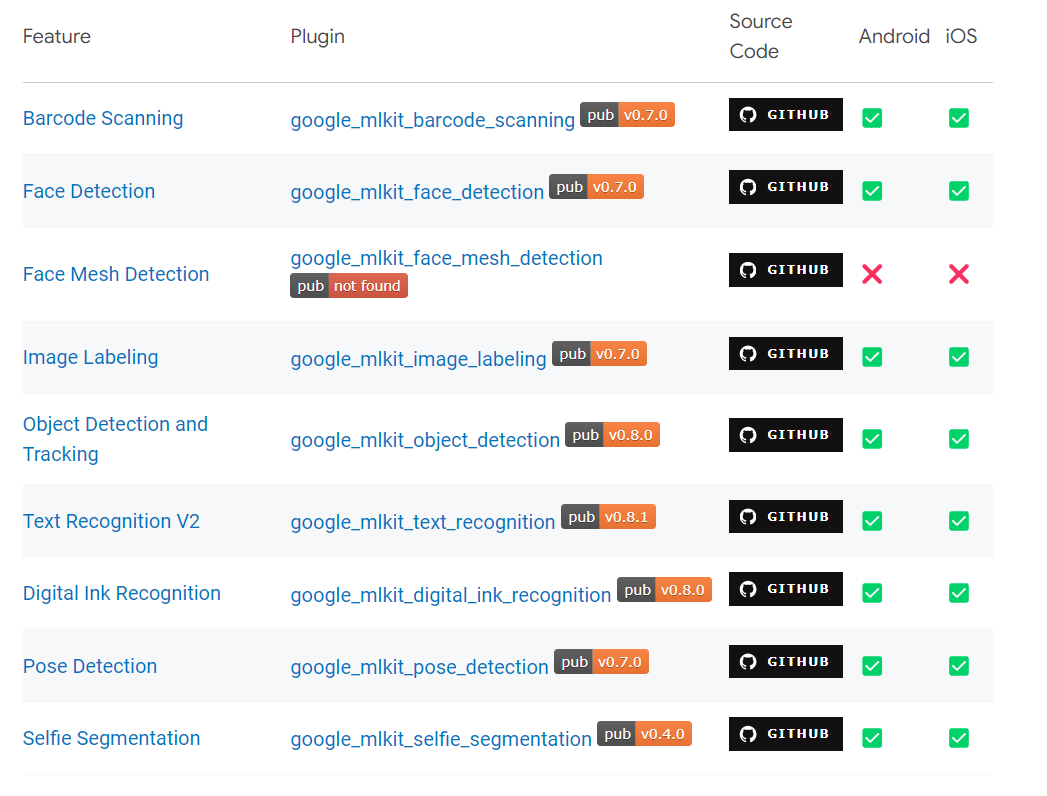
\includegraphics[width=1\textwidth]{imagenes/google_ml_kit.png}
    \caption{Herramientas ofrecidas por Google ML Kit}
\end{figure}

Al instalar dicha dependencia en el fichero de dependencias de nuestra aplicación, no se percibió ningún problema, excepto un excesivo tiempo de carga debido a la gran cantidad de plugins que contiene. Sin embargo, se continuó en la implementación del escaneado de tickets de la compra. Una vez desarrollada la funcionalidad en cuanto a programación se refiere, a la hora de testearla, se comenzó a notar que la aplicación no funcionaba del todo bien, en concreto la conexión con la base de datos de Firebase, además de mostrar el siguiente error cada vez que se realizaba alguna conexión con dicha base de datos:

\textcolor{red}{'This typically indicates that your device does not have a healthy Internet connection at the moment. The client will operate in offline mode until it is able to successfully connect to the backend.'}

\newpage

En principio, como se podría suponer por la traducción al español del error ofrecido por Flutter, se pensó que era culpa de la conexión a Internet pero, tras hacer varias pruebas con otros sitios web se llegó a la conclusión de que este no era el problema.

Tras indagar bastante, se dio con el problema. Como se puede ver en la imagen anterior, no todos los plugins de Google ML Kit están disponibles para sistemas operativos de dispositivos móviles, pues la funcionalidad \textit{Face Mesh Detection} no tiene soporte ni para iOS ni para Android. Esto hacía que la aplicación no se construyese de manera correcta, dando errores que se trasladaban, también, a las peticiones de la base de datos de Cloud Firestore.

Para solucionarlo, se puede ver en la segunda columna de la imagen anterior que cada dependencia de Google ML Kit se puede instalar por separado. Esto, además de solucionar el error de compatibilidad de plugins que no estabamos utilizando, permitía rebajar en gran medida la cantidad de dependencias que instalaba Google ML Kit, quedándose únicamente instalada en la aplicación Google ML Kit Text Recognition.

\section{Despliegue de la aplicación}

\subsection{Importancia}

Una parte esencial del desarrollo de cualquier aplicación, del tipo que sea, es su puesta en producción o despligue, ya con esto se brinda acceso directo a los usuarios. Esto significa que la aplicación estará disponible en las tiendas de aplicaciones, lo que permite que un público amplio pueda descargarla y comenzar a utilizarla. Esto es especialmente relevante en el entorno actual, donde los dispositivos móviles son ampliamente utilizados y las aplicaciones móviles son una parte integral de la vida cotidiana de muchas personas.

Además, desde el punto de vista económico, poner en producción una aplicación móvil es un paso crucial para obtener un retorno de inversión. Después de invertir tiempo, recursos y esfuerzo en el desarrollo de la aplicación, es necesario lanzarla al mercado para que pueda generar beneficios. Esto puede incluir ingresos por compras en la aplicación, publicidad, suscripciones, o cualquier otro modelo de monetización que se pueda establecer.

Esto no solo es importante en el ámbito económico, sino que se abre la puerta para recibir comentarios y opiniones de los usuarios reales. Esto es imprescindible para identificar áreas de mejora, solucionar problemas que a lo mejor no surgieron en la etapa de desarrollo y agregar nuevas funcionalidades en futuras actualizaciones. El feedback de los usuarios es esencial para comprender sus necesidades, preferencias y expectativas, y permite realizar ajustes que optimicen la experiencia del usuario y aumenten la satisfacción.

\subsection{Pasos a seguir para desplegar una aplicación con Flutter}

Para ello, en el sitio web oficial de Flutter \cite{despliegue} se pueden encontrar los pasos que se deben seguir a la hora de desplegar una aplicación en un entorno de producción, lo que se conocerá como una versión \textit{release}. Para ello, se han seguido los siguientes pasos:

\begin{enumerate}
    \item Revisar el fichero por defecto \textit{AndroidManifest.xml} localizado en el directorio \textit{\textless app dir \textgreater /android/app/src/main} y verificar si los valores son correctos, especialmente en la sección \textit{application}, editar \textit{android:label} para reflejar el nombre final de la aplicación.

    \newpage
    
    \item Añadir un icono para la aplicación. Este es un paso importante, pues distinguirá, a ojos del usuario, a la aplicación del resto, además de por el nombre. En el directorio \textit{\textless app dir\textgreater /android/app/src/main/res/}, se deben colocar los archivos de los iconos en las distintas resoluciones en la carpeta correspondiente, utilizando la misma nomenclatura que la que nos encontramos en los ficheros ya existentes.

    El logo de la aplicación ha sido diseñado utilizando la web Looka \cite{Lookah} que, usando inteligencia artificial y mediante una serie de parámetros introducidos como el estilo, el nombre y el tipo de marca sobre la que se trabaja, nos da una serie de logotipos entre los cuales podemos elegir el que queramos y modificarlo a nuestro gusto.

    \item Generar una clave de firma: Para publicar la aplicación en las tiendas oficiales, es necesario generar una clave de firma. Esto se logra mediante el uso de herramientas como \textit{keytool} para generar la clave, la cual deberá ser almacenada de forma segura.

    \item Configurar la firma de la app editando el archivo \textit{\textless app dir\textgreater /android/app/build.gradle}. Tras esto, todas las versiones \textit{release} que se construyan se firmarán automáticamente.

    \item Finalmente, se construye la versión de la aplicación para obtener el fichero en formato APK. Este formato es instalable en cualquier dispositivo Android, lo que nos permitirá, tanto instalar la aplicación en cualquier dispositivo con este sistema operativo de manera manual, como publicarla en las tiendas oficiales. Para ello, basta con ejecutar el comando \textit{flutter build apk}, el cual nos generará el fichero \textit{\textless app dir\textgreater /android/app/outputs/apk/release/app-release.apk}.
\end{enumerate}

Con estos pasos, ya se tendría una versión de la aplicación lista para probar en cualquier dispositivo Android, lo cual se ha utilizado para testear la aplicación en las distintas fases de su desarrollo tanto por parte del desarrollador y del tutor, como por parte de familiares y amigos, lo cual ha permitido a la aplicación retroalimentarse del feedback y opiniones de los mismos para seguir mejorando.

Sin embargo, a pesar de que la aplicación es multiplataforma y, al estar hecha en Flutter, también ha sido desarrollada simultáneamente para dispositivos iOS, no se ha podido desplegar una versión en producción para los mismos, pues Apple solo permite la compilación de aplicaciones de este sistema operativo en ordenadores con ese mismo software. Además, para publicar aplicaciones en su tienda oficial, el App Store, es necesario darse de alta en el Apple Developer Program, lo cual, como se ha comentado en el punto 1.4 de este mismo documento, cuesta unos \$99 al año, lo que viene siendo unos 92 euros anuales.

\section{Demostración de la aplicación}

En el siguiente apartado, se llevará a cabo un exhaustivo análisis de los diversos apartados de la aplicación, detallando minuciosamente su funcionamiento. Además, se proporcionará una valiosa visualización de la interfaz de usuario final a través de una captura de pantalla. El propósito fundamental de esta exploración es lograr una comprensión más profunda del trabajo realizado y del rendimiento de la aplicación en términos de experiencia de usuario. De esta manera, se busca obtener una visión integral y enriquecedora que permita apreciar de manera completa y precisa todos los aspectos relacionados con su funcionamiento y usabilidad.

Asimismo, al culminar esta sección, se exhibirán una serie de ejemplos verificados en tickets de diversos establecimientos. Estos ejemplos servirán para ilustrar el grado de fiabilidad que esta funcionalidad es capaz de brindar, acompañados de una detallada explicación sobre tanto sus beneficios como sus limitaciones. De este modo, se busca proporcionar un respaldo empírico que respalde la eficacia del sistema, al tiempo que se abordan de forma transparente tanto sus fortalezas como sus puntos a mejorar.

\subsection{Inicio}

A continuación se detallarán los distintos apartados que se corresponden con los componentes clave de los apartados de inicio de sesión y registro, lo cual es lo primero que se puede encontrar al abrir la aplicación. Esto incluye la forma en que los usuarios interactúan con la aplicación para acceder a su cuenta o crear una nueva, las medidas de seguridad implementadas para proteger la información personal y las opciones adicionales que pueden ofrecerse para mejorar la experiencia del usuario, como el recordatorio de credenciales, la verificación del correo electrónico o la modificación de la contraseña.

Es importante destacar que tanto el proceso de inicio de sesión como el de registro están diseñados para ser intuitivos y accesibles para los usuarios. Esto implica la presentación clara de campos de entrada de datos, opciones de recuperación de contraseña y la posibilidad de autenticarse a través de servicios externos como podrían ser otras redes sociales.

\subsubsection{Inicio de sesión}

Al acceder a la pantalla de inicio de sesión, se muestra el distintivo logo de la aplicación, brindando una identificación visual única que diferenciará la aplicación del resto a simple vista. Este logo, como se ha mencionado anteriormente, ha sido diseñado utilizando la web \textit{}, respetando un diseño minimalista que representa una aplicación destinada a listas de la compra y manteniendo el color azul distintivo de la aplicación.

\begin{wrapfigure}{l}{0.35\textwidth}
    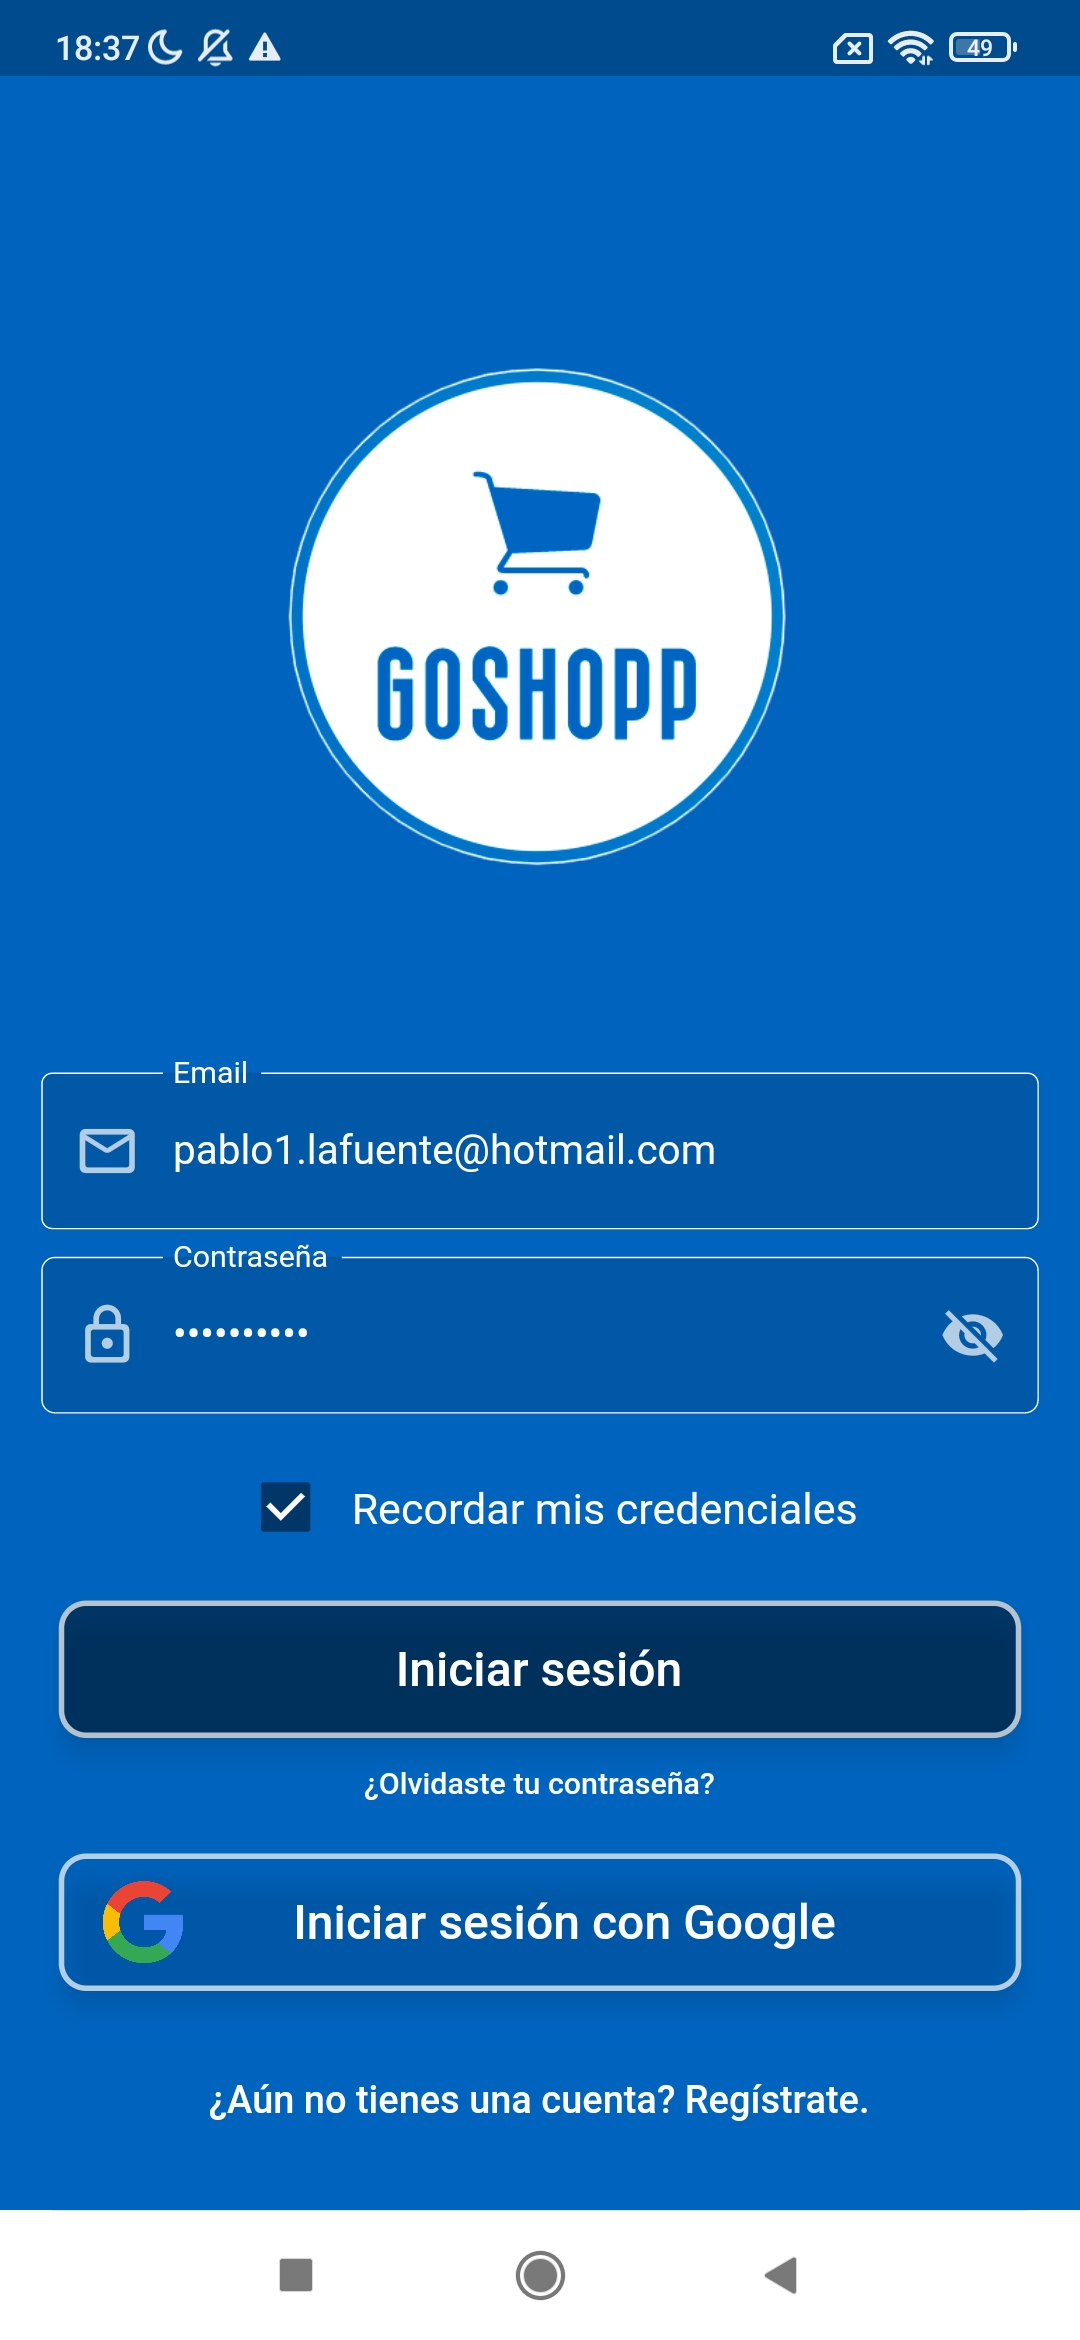
\includegraphics[width=0.32\textwidth]{imagenes/pantallas/inicio/login.jpg}
    \caption{Login}
    \vspace{-2\intextsep}
\end{wrapfigure}

A continuación se encuentran los campos correspondientes para ingresar la dirección de correo electrónico y la contraseña de una cuenta ya creada previamente. Estos campos permiten a los usuarios proporcionar sus credenciales de acceso de forma segura, pues la contraseña se mantiene oculta a menos que el propio usuario pulse el botón que habilita su contiendo, referenciado con el icono de un ojo. De esta forma el usuario podrá iniciar sesión de forma tradicional, siempre y cuando ya cuente con las credenciales de una cuenta existente en la base de datos del sistema.

Además, se ofrece al usuario la posibilidad de recordar credenciales mediante una casilla de verificación, que facilita el acceso posterior al recordar la información de inicio de sesión. Si el usuario mantiene esta casilla marcada en el momento de iniciar sesión, el sistema guardará las credenciales introducidas y, cuando el usuario vuelva a abrir la aplicación, estas aparecerán ya introducidas en el formulario de la parte superior. Esta función es especialmente conveniente para usuarios frecuentes que desean agilizar el proceso de autenticación.

También se puede encontrar un botón el cual el usuario puede pulsar en caso de haber olvidado su contraseña, el cual le llevará a otra pestaña en la que se le mostrará un cuadro de texto pidiendo el correo electrónico de su cuenta. Por tanto, el email que el usuario introduzca al momento del registro debe ser verídico. Para ello se ha implementado un método de verificación de correo electrónico que se explicará posteriormente. Una vez el usuario solicite una nueva contraseña, se le enviará un correo electrónico a la dirección introducida con un enlace que le permitirá acceder a un formulario donde modificar la contraseña a la nueva que desee, con la cual podrá volver a acceder a la aplicación sin ningún problema, desechando la contraseña antigua.

Sin embargo, no es estrictamente necesario que el usuario inicie sesión utilizando el método tradicional. Como se ha explicado en la arquitectura interna de la autenticación de usuarios, la aplicación ofrece la posibilidad de iniciar sesión con una cuenta de Google ya existente. Al pulsar en el botón indicado para ello, aparecerá un modal para abrir cualquiera de las cuentas de Google guardadas en nuestro dispositivo o, en el caso de que solo exista una, se iniciará la sesión automáticamente con ella.

Finalmente, en la parte inferior de la pantalla, encontramos un botón que permite al usuario registrar una nueva cuenta en el sistema. Al hacer clic en este enlace, los usuarios son redirigidos a una página donde podrán crear una nueva cuenta en la aplicación. El proceso de registro puede incluir campos adicionales para recopilar información personalizada, según los requisitos de la plataforma, para mejorar de esta forma la experiencia de usuario de la misma.

La necesidad de autenticarse de forma segura antes de acceder a la plataforma es esencial para garantizar la protección de los datos y la privacidad del usuario. Como es obvio, sin iniciar sesión correctamente, el usuario no podrá acceder a las funciones, características y contenido personalizado que ofrece la aplicación.

A continuación se muestran algunas capturas de pantalla que se corresponden con la verificación de correo electrónico y la recuperación de contraseña, así como la página de registro de usuarios que se procederá a explicar a continuación:

\vspace{0.5cm}
\begin{figure}[htbp]
    \centering
    \begin{minipage}[h]{0.32\textwidth}
        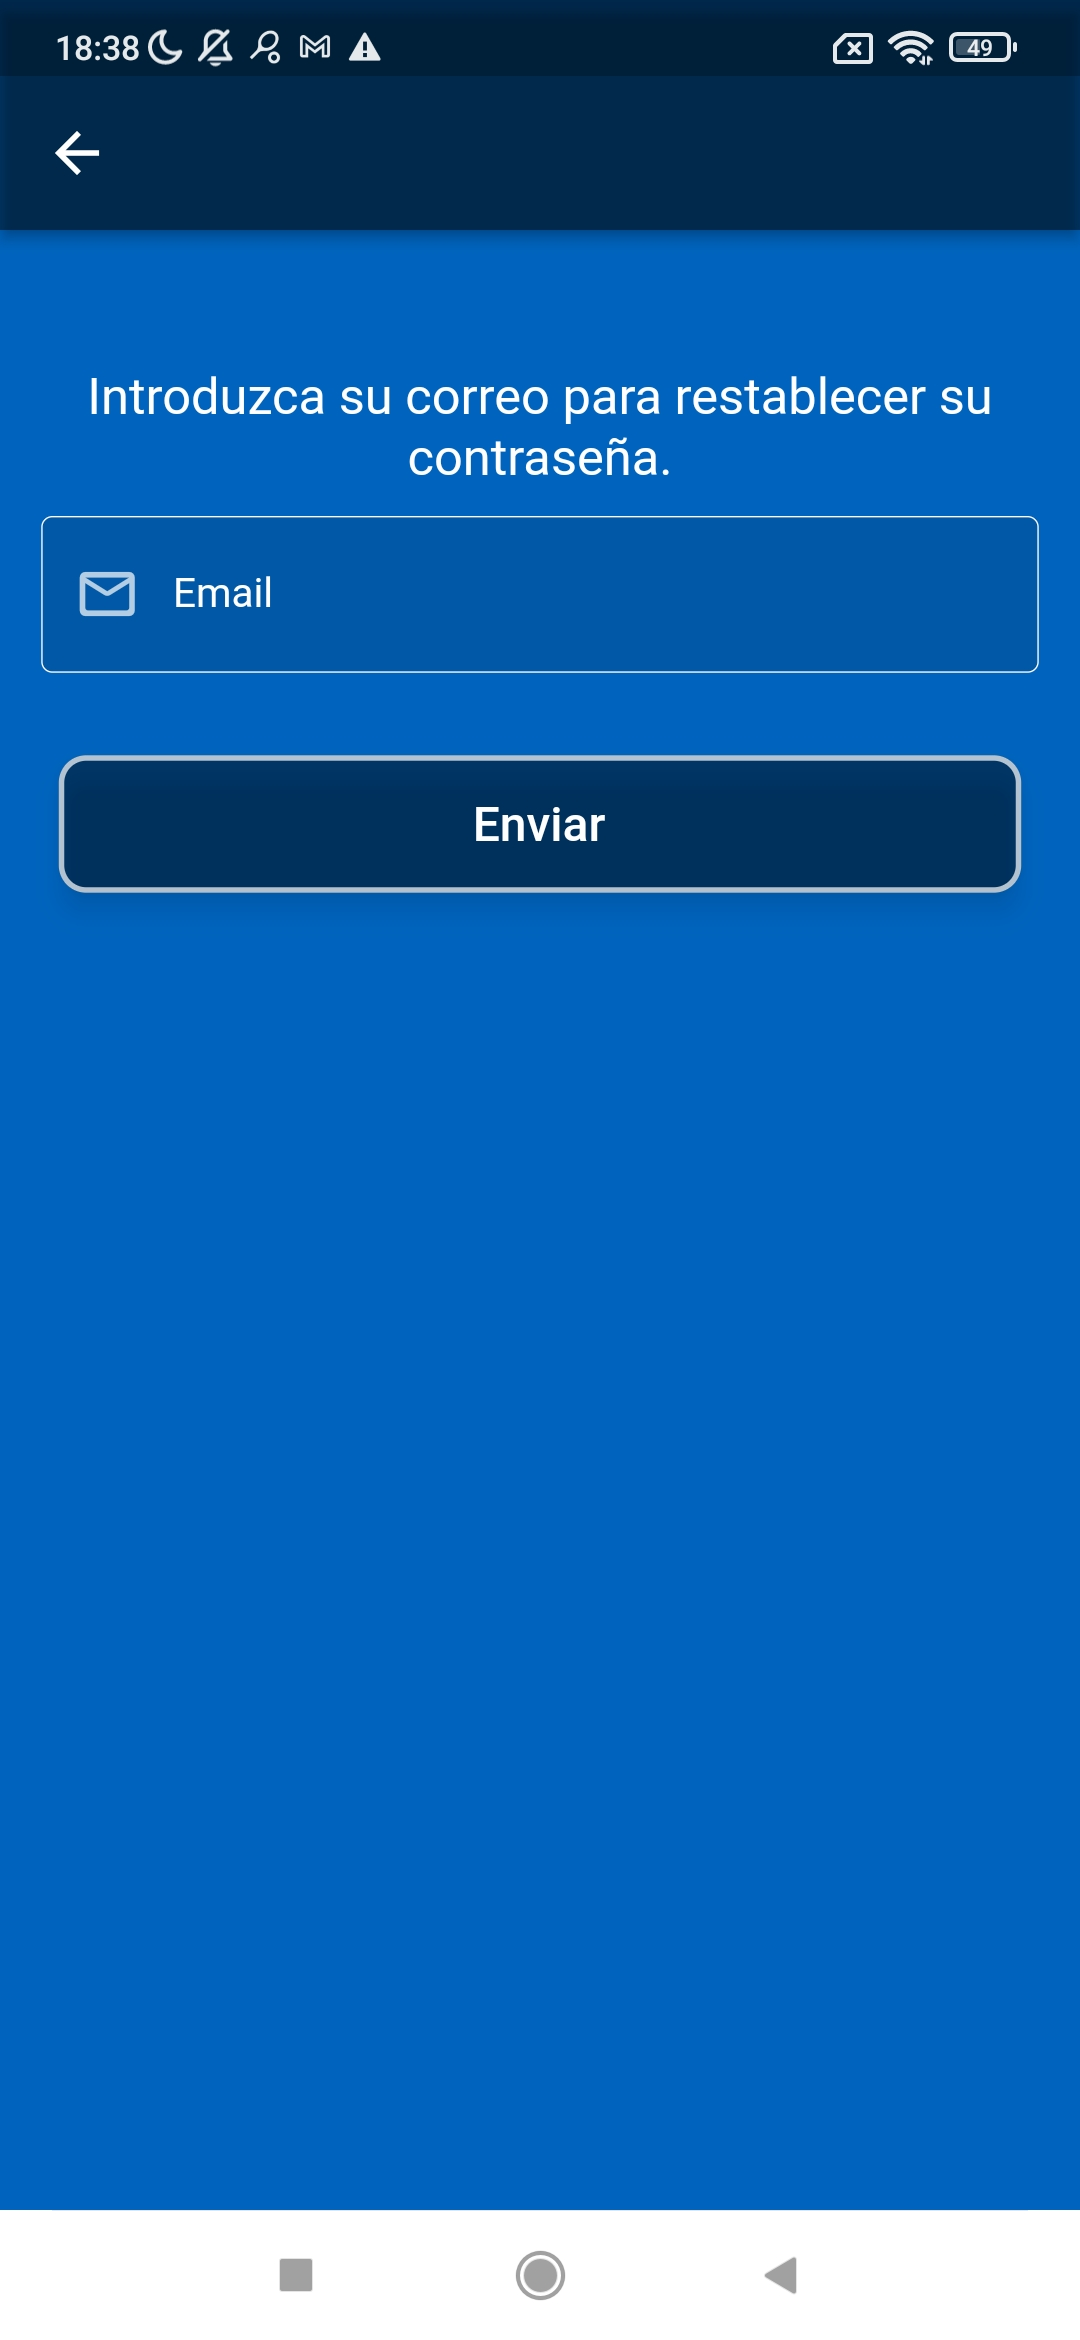
\includegraphics[width=\textwidth]{imagenes/pantallas/inicio/recordar_contrasena.jpg}
        \caption{Recordar contraseña}
    \end{minipage}
    \hfill    
    \begin{minipage}[h]{0.32\textwidth}
        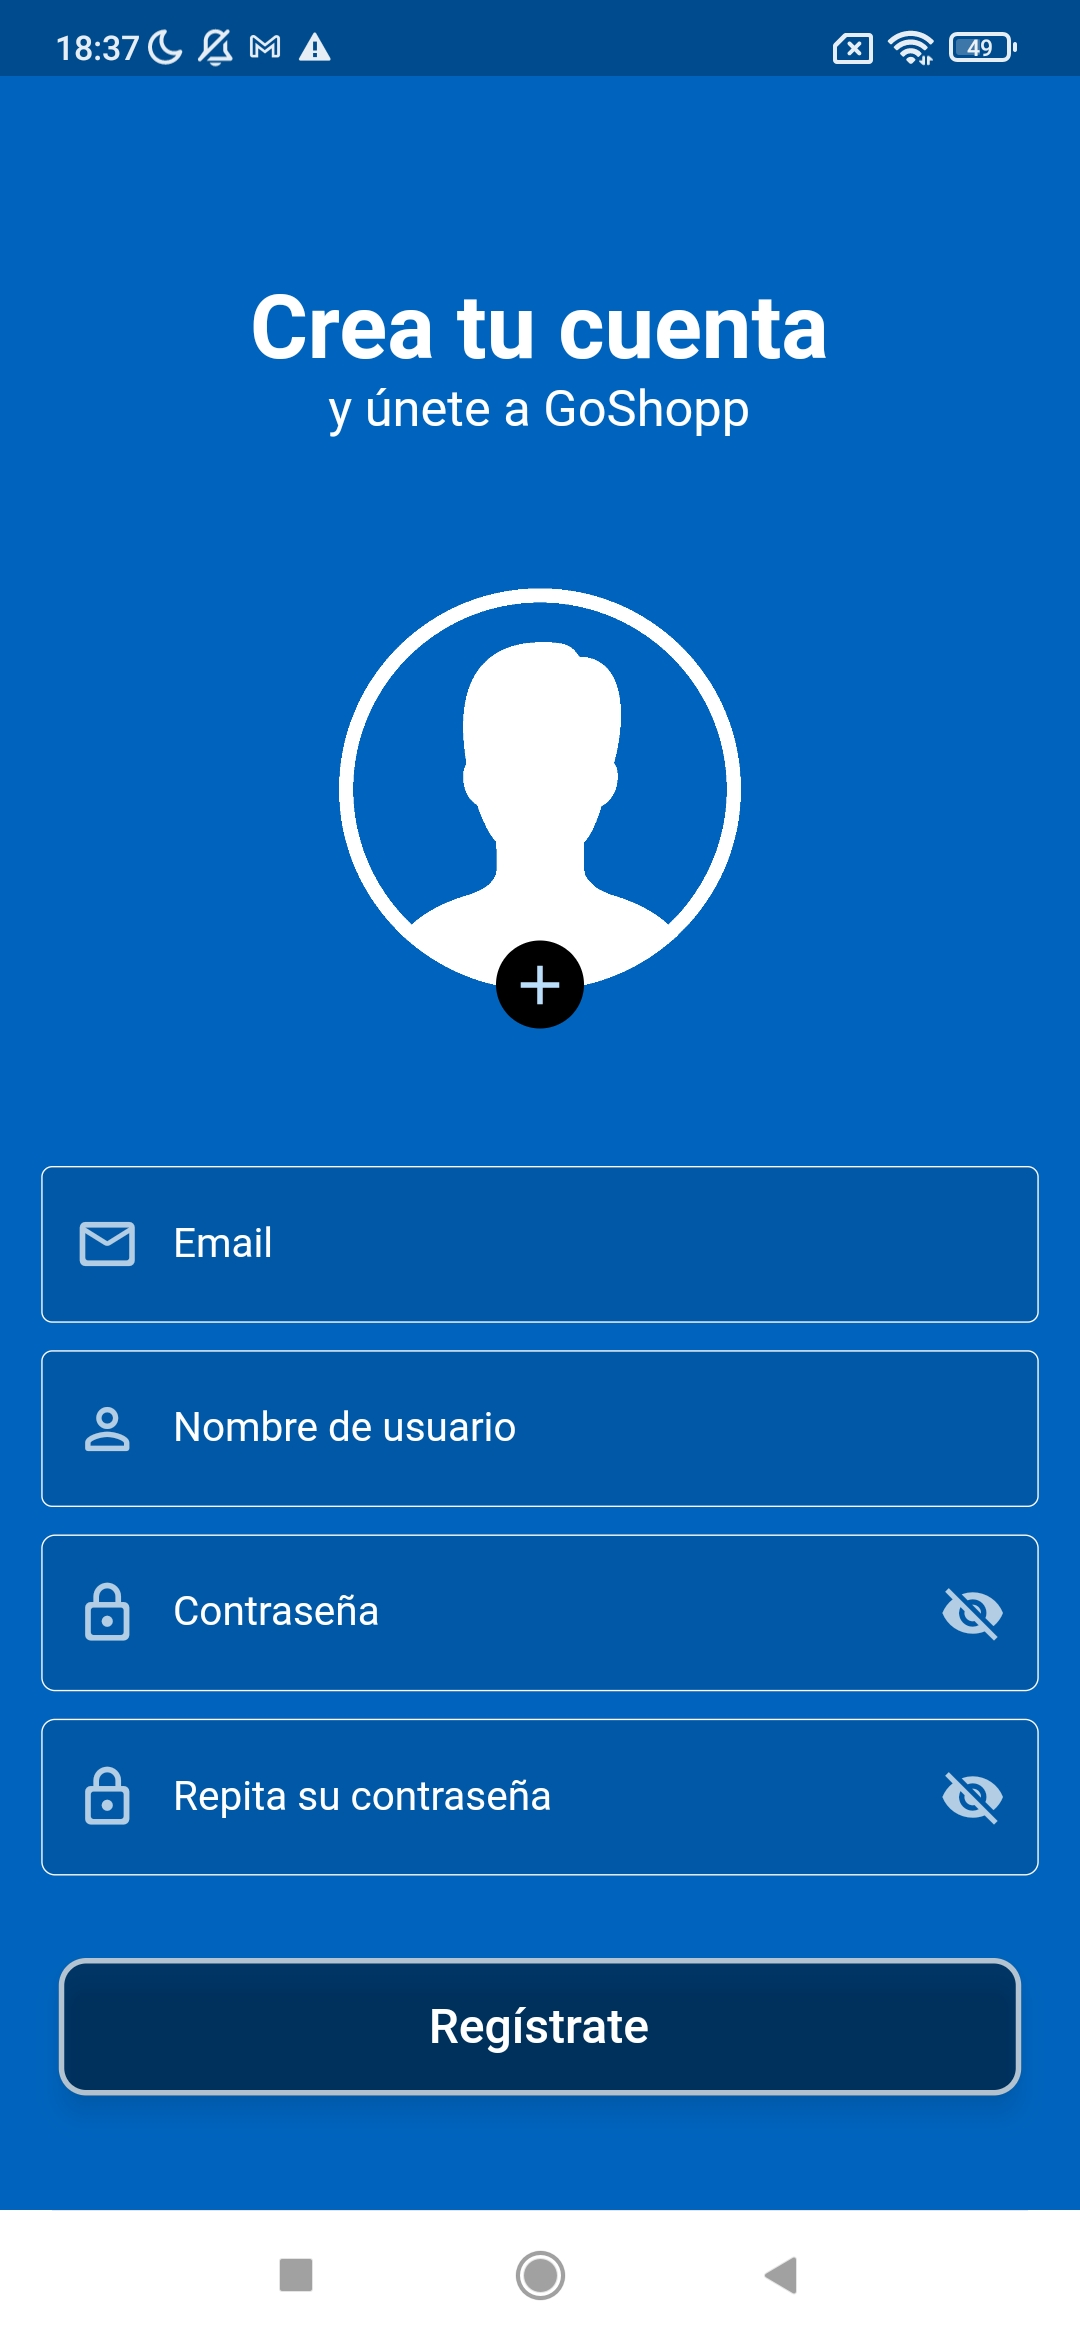
\includegraphics[width=\textwidth]{imagenes/pantallas/inicio/registro.jpg}
        \caption{Registro de usuarios}
    \end{minipage}
    \hfill
    \begin{minipage}[h]{0.32\textwidth}
        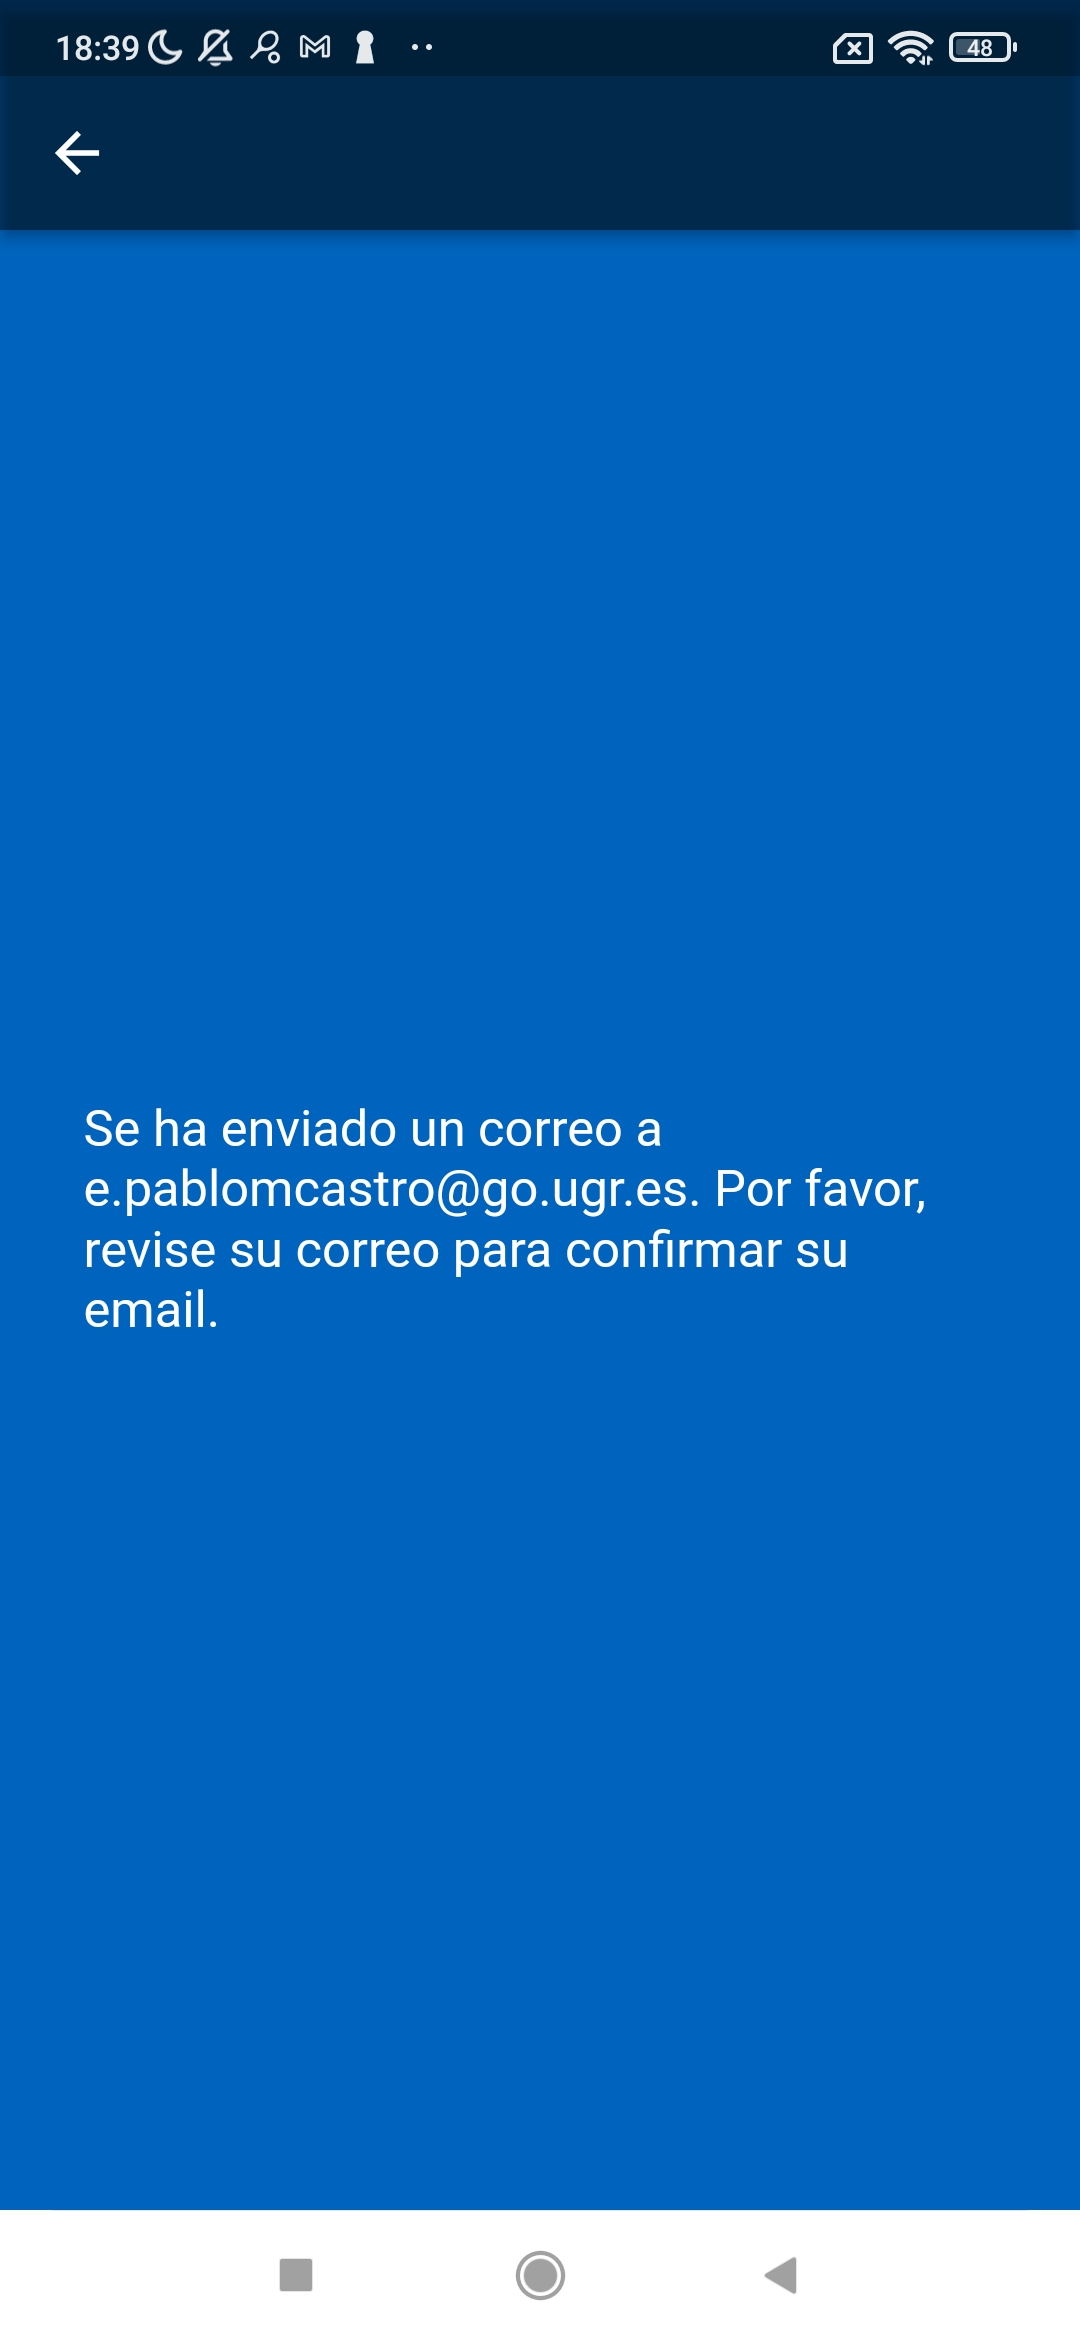
\includegraphics[width=\textwidth]{imagenes/pantallas/inicio/verificar_correo.jpg}
        \caption{Verificación de email}
    \end{minipage}
\end{figure}

\newpage

\subsubsection{Registro de usuarios}

Al abrir la pantalla de registro, se muestra un mensaje de bienvenida en la parte superior, donde se da la bienvenida al usuario y se le anima a unirse a la comunidad, proporcionando así una imagen amigable de la aplicación de cara al usuario. Todos los campos proporcionados al usuario en esta pantalla, como se ha mencionado anteriormente, realizan internamente una serie de validaciones, informando al usuario en caso de éxito o de error en todo momento.

Justo debajo del mensaje de bienvenida, se encuentra un espacio reservado para la foto de perfil del usuario. Este campo se muestra inicialmente vacío, representando dicho vacío con una imagen de la sombra de lo que podría ser una foto de perfil en primer plano de una persona. Al hacer clic en el botón indicado para tal fin, se abre una opción para cargar una imagen desde el dispositivo del usuario. Una vez seleccionada la imagen, esta se muestra en el campo de la foto de perfil, sustituyendo la imagen anterior, permitiendo al usuario ver una vista previa de cómo se verá su foto en su cuenta. En caso contrario, si el usuario abandona el menú de selección de una imagen, se le mostrará un mensaje indicando que no se ha seleccionado ninguna, y la imagen mostrada seguirá siendo la misma. Cabe destacar que, para que todas las imágenes se muestren en el mismo formato, se modifican al momento de la visualización para que tomen una forma redonda, independientemente de su forma o tamaño originales.

A continuación, se presentan varios campos de entrada de texto. El primero es el campo de nombre de usuario, donde el usuario puede ingresar un nombre que lo identifique en la plataforma. Sin embargo, a diferencia de lo que ocurre en otras aplicaciones, este nombre de usuario no necesariamente debe ser único, pues los usuarios serán identificados internamente mediante su correo electrónico.

Justo debajo del campo de nombre de usuario, se encuentra dicho campo de correo electrónico, donde el usuario debe ingresar su dirección de correo electrónico válida. En este caso, no se comprobará que la dirección introducida exista o no, pero no se le permitirá al usuario entrar a la aplicación hasta que no la verifique una vez registrado, por lo que deberá asegurarse de que el correo electrónico introducido existe y tiene acceso al mismo.

A continuación, se presentan dos campos en los que el usuario deberá introducir su contraseña. El primero es el campo de contraseña, donde se debe ingresar la contraseña deseada. Junto a este campo, se coloca un pequeño icono de un ojo, al igual que en el de inicio de sesión, que permite al usuario alternar entre la visibilidad de la contraseña, mostrándola como texto plano sin ocultar, o su ocultamiento, sustituyendo cada carácter por un punto negro, como suele ser habitual en estos casos. El segundo campo es el campo de repetir contraseña, donde el usuario debe ingresar nuevamente la contraseña anteriormente ingresada para confirmarla. Esta confirmación ayuda a evitar errores de escritura y asegura que el usuario haya ingresado correctamente la contraseña deseada.

Finalmente, en la parte inferior de la pantalla, se muestra un botón para enviar el formulario ya rellenado. Al hacer clic en este botón, se procesa la información ingresada por el usuario para completar el proceso de registro y crear su cuenta. Si todo ha ido correctamente, se informará al usuario y se le redirigirá a una nueva página, sin permitirle aún acceder al contenido de la aplicación.

Se ha mencionado que el correo electrónico debe ser válido y existente, ¿a qué se debe esto? Bien, una vez el usuario se ha registrado correctamente y no hay errores de validación en el formulario, se le enviará un correo electrónico a la dirección introducida, el cual contendrá un enlace para verificar la cuenta. No se permitirá el acceso al resto de la aplicación hasta que el usuario haya pulsado en dicho enlace. Esto lo que permitirá al sistema es asegurarse de que la dirección de correo electrónico es real, no permitiendo así que un usuario se invente correos electrónicos para tener múltiples cuentas en nuestro servidor.

\newpage

Una vez el usuario ha verificado su dirección de correo, automáticamente la aplicación le redirigirá a la página principal, no teniendo que volver a pasar por este proceso nunca más si inicia sesión con la cuenta creada. Cabe destacar también que, si un usuario crea una cuenta pero no verifica el email, y sale de la aplicación, cuando vuelva a acceder a ella podrá iniciar sesión, pero se le volverá a mostrar el mensaje anteriormente mencionado y no podrá acceder a la aplicación a menos que verifique su dirección de correo electrónico como se ha explicado anteriormente.

\subsection{Listas de la compra personales}

Una vez se le concede acceso al usuario a la aplicación, lo primero que ve al iniciar sesión es una pantalla con dos pestañas en la parte superior, en la que se puede alternar entre mostrar las listas de la compra personales del propio usuario o el listado de grupos a los que pertenece el mismo. Vamos a comenzar hablando del primer caso, adentrándonos por completo en la funcionalidad de nuestra aplicación relacionada con las listas de la compra, pues en el caso de las listas cooperativas, funciona exactamente igual.

Justo en el momento en el que el usuario accede a esta pestaña, se realiza una consulta a la base de datos que obtiene todas las listas de la compra personales asignadas al usuario en cuestión. Para ello, la aplicación se limita a obtener todos los documentos de la colección 'listas' asignada al usuario que se encuentra activo en la aplicación. Durante este proceso, se muestra un circulo de carga que indicará al usuario que sus listas de la compra está siendo recuperadas.

Una vez finalizada dicha consulta, se mostrará un mensaje indicando que no existen aún listas de la compra disponibles para dicho usuario, y se le anima, de forma amigable, a que comience a crear listas de la compra para aprovechar todo el potencial que ofrece la aplicación. Para ello, se puede ver fácilmente un botón en la parte superior, justo encima del circulo de carga o, en su defecto, del mensaje informativo, que permite al usuario crear una nueva lista. Este botón redirigirá al usuario a un formulario en el cual se profundizará más adelante.

En caso de que sí se hayan obtenido las listas de la compra personales del usuario, estas aparecerán justo debajo de dicho botón. El usuario podrá deslizar hacia abajo en el caso de que haya más de las que la pantalla del dispositivo en cuestión permita ver, permitiéndole no perder en ningún momento información del resto de la pantalla mientras desliza buscando la lista deseada. Cada lista, se muestra como un widget independiente para Flutter, de forma que, una vez que se ha obtenido de la base de datos una especie de vector con todas las listas que pertenecen al usuario, se recorre creando un nuevo widget, hijo del contenedor donde aparece dicho listado, con la información independiente de cada lista de la compra.

Para la representación de cada una de las listas de la compra, se ha querido elaborar un diseño que impacte a ojos del usuario y llame la atención, pues se trata de la funcionalidad principal de la aplicación, sin despegarse de los tonos azules característicos de la misma. Para ello, el widget se ha diseñado con un contorno cuadrado, con los bordes de las esquinas redondeados, dándole así un toque estético. Para el fondo, se ha utilizado un tono de azul mucho más oscuro, que no llega a ser negro, para llamar la atención a ojos del usuario, mostrando el nombre de la lista en la parte superior, junto con dos iconos que actuarán como botones de edición y eliminación de la lista. Justo debajo, y en un color ya más en concordancia con el color primario de la aplicación, se ha diferenciado la descripción, para brindar más información aún al usuario.

\begin{figure}[h]
   \centering
    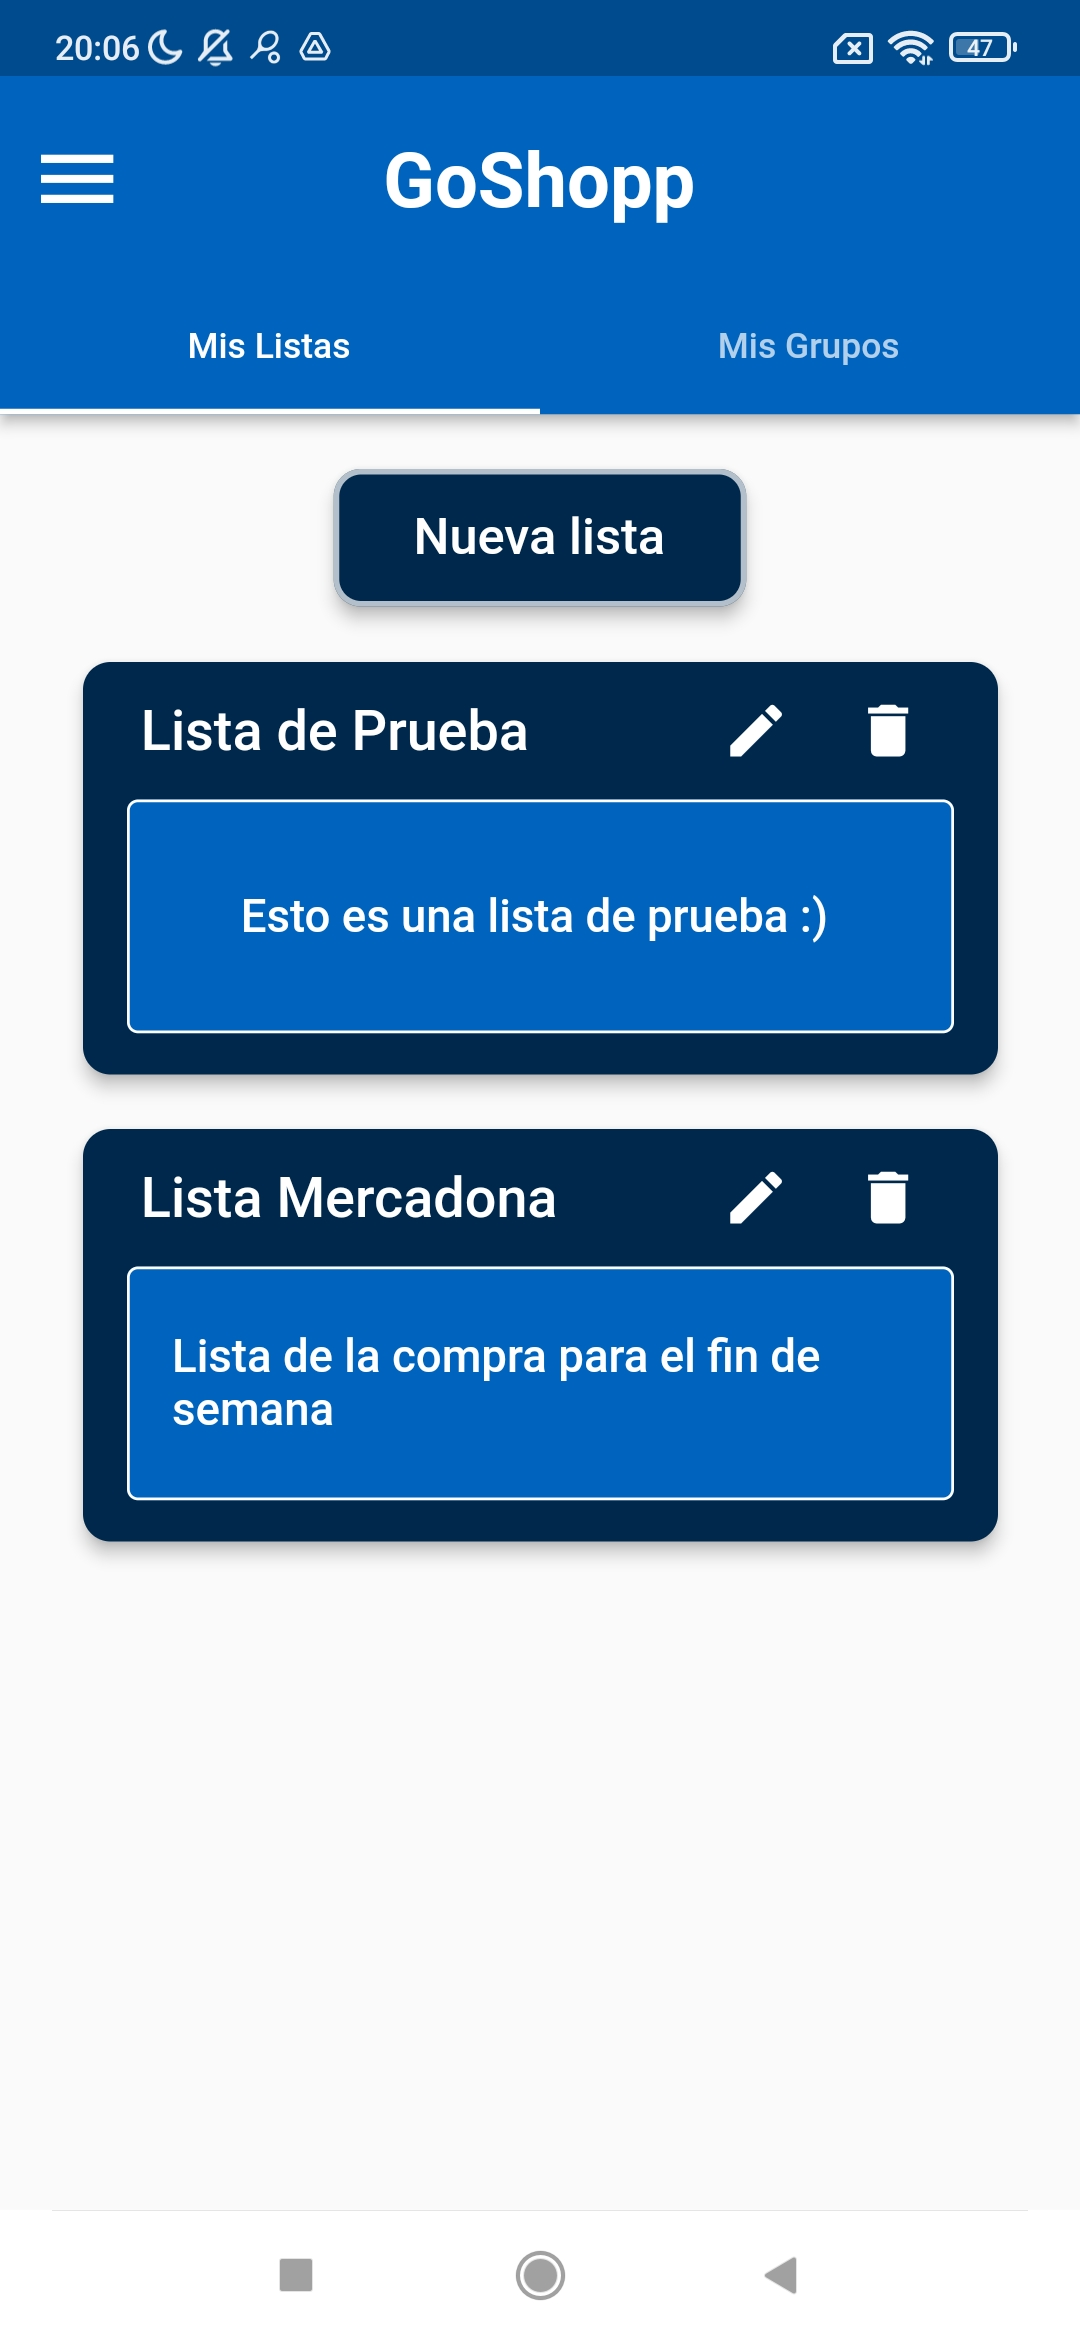
\includegraphics[width=0.35\textwidth]{imagenes/pantallas/listas/listas.jpg}
    \caption{Listas personales}
\end{figure}

\subsubsection{Editar una lista de la compra}

El primer botón, con el icono de un lápiz, nos abre una pantalla que en la que se exhibe un formulario compuesto por un campo de texto destinado al título de la lista y otro campo de texto más extenso para la descripción de la misma. Además, se incluye un botón que permite la creación de la lista.

El campo de texto para el título de la lista se encuentra posicionado en la parte superior del formulario. Su función es permitir al usuario editar el título deseado para la lista, respetando un tamaño máximo establecido en 20 caracteres, el cual se ha considerado adecuado para facilitar la legibilidad y la edición del texto, así como su posterior visualización en el widget correspondiente. Para evitar que el usuario tenga que contar los caracteres que lleva escritos, se proporciona un contador que indica, hasta 20, el número de caracteres introducidos por el usuario en tiempo real.

Justo debajo del campo de texto del título se encuentra el campo de texto más extenso, diseñado para alojar una descripción detallada de la lista. Esta área de texto proporciona un espacio amplio en el cual el usuario puede ingresar una cantidad considerable de texto, tanto en una sola línea como en varias líneas, para puntualizar de una forma concreta el objetivo hacia el cual se destina dicha lista, para su posterior mejor comprensión tanto por el mismo como por el resto de usuarios, si se trata de una lista grupal.

Cabe destacar que, en el momento en el que el usuario acceda a dicho formulario para editar una lista de la compra, este se encontrará ya relleno con los valores actuales tanto del título de la lista, el cual es obligatorio, como por la descripción, en caso de que la tenga. También es importante aclarar que, en caso de dejarse vacío el primer campo y querer editar la lista, no será posible y se mostrará un mensaje de error indicando dicho problema.

En cuanto al botón de edición de la lista, se sitúa bajo el campo de texto de la descripción. Su función principal es iniciar el proceso de creación de la lista, utilizando los datos ingresados en los campos de texto mencionados anteriormente. Este botón se presenta de manera prominente, respetando el patrón de diseño seguido en toda la aplicación, con el fin de que sea fácilmente identificable y accesible para el usuario.

El usuario también tiene la posibilidad de volver atrás sin guardar los cambios realizados en la lista de la compra mediante el botón situado en la parte superior, en el que se puede ver la típica flechita común en estos casos que indica el retorno a la página anterior.

\subsubsection{Borrar una lista de la compra}

Volviendo a la pantalla principal de la aplicación, se va a proseguir explicando el contenido del widget que muestra la información de cada lista. El botón situado a la derecha del de edición de listas, representado por el icono de una papelera, se encargará de la funcionalidad de eliminar una lista. Al pulsar el usuario sobre él, abrirá un pequeño modal pidiendo al usuario confirmación de si quiere o no realmente borrar la lista, evitando así posibles eliminaciones indeseadas en caso de que el usuario pulse dicho botón por error.

Si la respuesta al modal de confirmación es positiva, se indicará pulsando el botón azul, tras lo cual la lista se eliminará de nuestra base de datos, eliminado así también todas las relaciones de productos asociados a la misma, y la pantalla se volverá a cargar actualizando su contenido, dejando de mostrar la lista recién borrada. En caso de que la respuesta del usuario sea negativa, se deberá indicar pulsando sobre el botón rojo, lo cual devolverá al usuario a la pantalla principal sin realizar ninguna modificación.

\begin{figure}[h]
    \centering
    \begin{minipage}[h]{0.33\textwidth}
        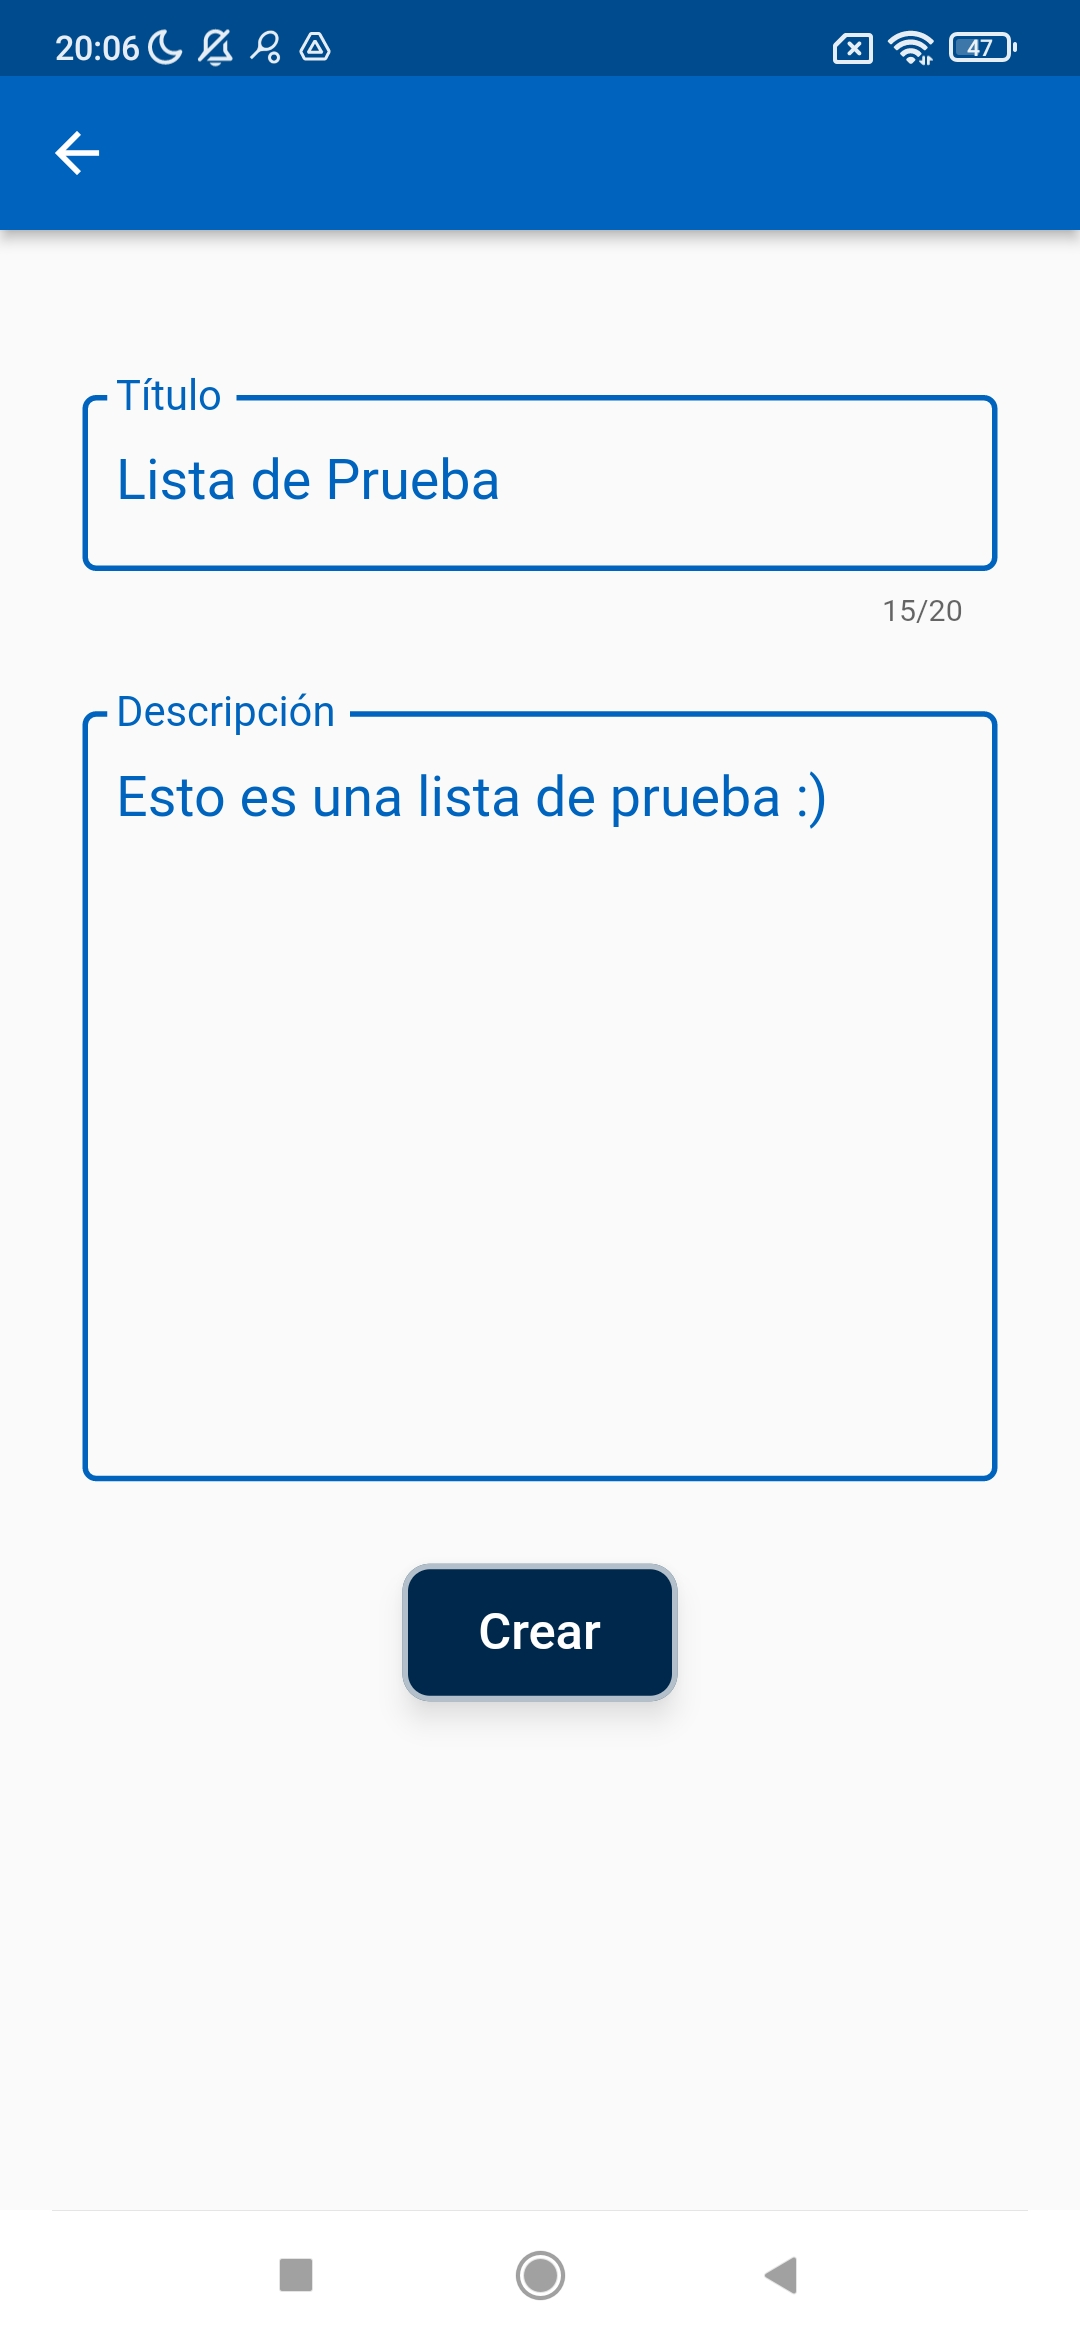
\includegraphics[width=\textwidth]{imagenes/pantallas/listas/crear_lista.jpg}
        \caption{Crear/editar una lista}
    \end{minipage}
    \hspace{1cm}
    \begin{minipage}[h]{0.33\textwidth}
        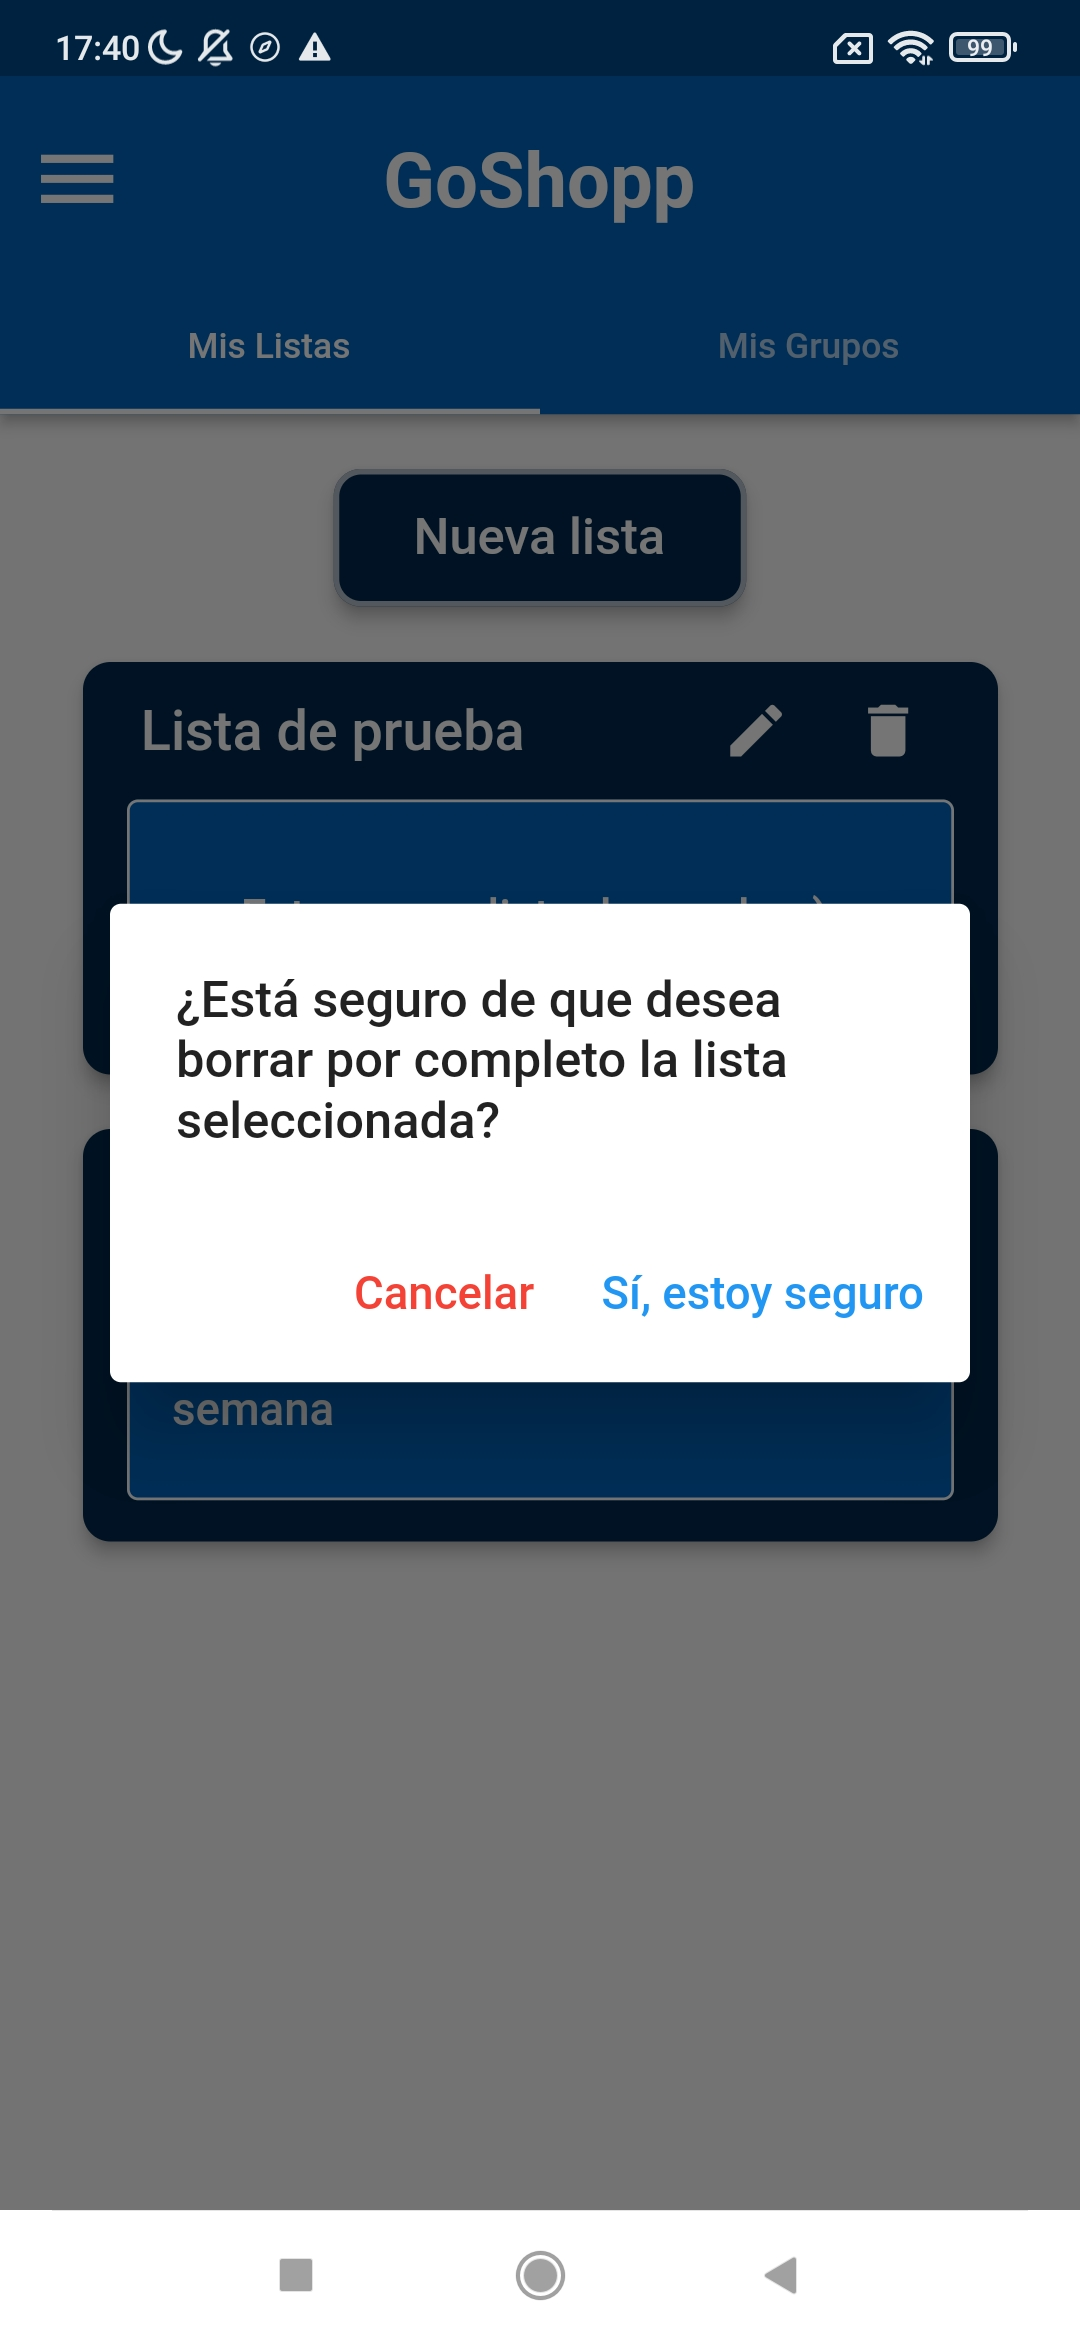
\includegraphics[width=\textwidth]{imagenes/pantallas/listas/modal_borrar_lista.jpg}
        \caption{Borrar una lista}
    \end{minipage}
\end{figure}

\subsubsection{Crear una lista de la compra}

Independientemente de si el usuario posee o no listas de compra asociadas, siempre se le brindará la opción de crear nuevas listas, ya sean individuales o grupales. En este contexto, se detallará el procedimiento para crear una lista personal o privada, dado que nos encontramos en esta sección.

Para iniciar el proceso de creación de una lista personal, el usuario deberá hacer clic en el botón designado para tal fin, tal y como se explicó previamente. Este botón, claramente identificado, representa la acción de crear una lista y se encuentra fácilmente accesible en la interfaz de usuario.

Al hacer clic en dicho botón, se desplegará un formulario que permitirá al usuario ingresar tanto el nombre de la lista como una descripción que facilite su identificación. Es importante destacar que para esta funcionalidad se ha reutilizado el mismo formulario utilizado para la edición de listas, pero con la particularidad de que en esta instancia ambos campos aparecerán vacíos, listos para que el usuario los complete.

Además, al visualizar el formulario, se podrá observar una modificación en el botón de confirmación. En lugar de mostrar el término \textit{Editar}, utilizado en el caso de formularios de edición, el botón ahora mostrará el término \textit{Crear}. Esta adaptación en el lenguaje del botón refuerza visualmente el propósito específico de la acción en curso, que es la creación de una lista nueva.

Con esta interfaz intuitiva y claramente diseñada, los usuarios podrán crear fácilmente sus propias listas de compra personalizadas, sin interferir con las listas de compra colaborativas pertenecientes a los grupos. Esta separación funcional garantiza la autonomía y la privacidad en la gestión de las listas personales de cada individuo.

\subsubsection{Ver contenido de una lista de la compra}

Al interactuar con cualquier punto del widget que contiene la información de cada lista de compra, se accede a una pantalla representada en la Figura \ref{fig:productos}. En esta pantalla, se muestra un listado detallado de todos los productos que han sido agregados a dicha lista, así como todas las funcionalidades posibles para las mismas.

Lo primero que se puede encontrar, en la parte superior de dicha pantalla, es el nombre de la lista. Esto permite una identificación rápida por parte del usuario de la lista sobre la que se está trabajando, para evitar equivocaciones. Junto a él, aparecen dos iconos. El primero, como se puede sobreentender, nos devuelve a la página anterior, mostrando de nuevo todas las listas del usuario, en caso de que el usuario quiera seguir trabajando sobre otra lista o acceder a un grupo una vez ha terminado de modificar la lista actual.

Siguiendo con la descripción de forma descendente, nos encontramos con la descripción de la lista, la cual se muestra aquí debido a que, tras recibir un primer feedback de algunos usuarios, se llegó a la conclusión de que podría resultar útil e informativa de cara al usuario.

\subsubsection{Añadir productos a una lista de la compra}

En la esquina superior derecha de la pantalla, se encuentra el segundo icono, que representa la función de escaneo. Al hacer clic sobre este botón, se le brinda al usuario la opción de seleccionar si desea obtener la imagen del ticket de compra desde la galería de su dispositivo, o si prefiere capturar una fotografía en tiempo real utilizando la cámara del dispositivo, apareciendo un modal como el mostrado en la Figura \ref{fig:modal}.

En ambas opciones, una vez confirmada la selección de la imagen, se llevará a cabo el escaneo de la misma, y los productos serán agregados a la lista de forma automática, como si hubiesen sido ingresados manualmente uno por uno, devolviendo al usuario a la pantalla actual.

Para añadir un producto a la lista de forma manual, tenemos justo debajo un formulario diseñado para tal fin, con el objetivo de tener un funcionamiento simple, intuitivo y que ocupe el menor espacio posible en la interfaz. Simplemente se debe ingresar el nombre del producto deseado en el cuadro de texto ubicado en la parte superior de la pantalla.

Este campo sigue el mismo formato que el del título de las listas al editar o crear, haciendo que la aplicación quede homogénea y facilite al usuario a la hora de intuir para qué sirve cada elemento de la misma. Además, es obligatorio, por lo que, en el caso de que el usuario añada un producto sin haberlo rellenado, se mostrará un mensaje de error indicando el problema.

A continuación, se elige el tipo de producto que se va a añadir utilizando el menú desplegable que se encuentra justo debajo del cuadro de texto, el cual nos ofrece un abanico de posibilidades bastante amplio. En caso de no hacerlo, el producto se añadirá por defecto siendo de tipo \textit{Comida}, pues se entiende que es el más común y utilizado en este tipo de aplicaciones, evitando así el trabajo del usuario de introducirlo manualmente en la mayoría de adiciones. Una vez seleccionado un tipo, se procede a pulsar el botón \textit{Añadir}. Al hacerlo, automáticamente se actualizará el listado de productos, mostrando el nuevo elemento junto a los existentes.

\subsubsection{Visualizar los productos añadidos a una lista de la compra}

Esta misma pantalla muestra un listado de productos, donde cada uno está representado por su nombre y su tipo. El primero se muestra en un tamaño de fuente más grande, lo que facilita su lectura y destacado en la lista. Justo debajo del nombre, se presenta el tipo de producto en un tamaño de fuente más pequeño, lo que proporciona información adicional sobre el producto en cuestión, sin llegar a ser tan relevante para el usuario a primera vista.

Cada producto se presenta en una línea separada, lo que permite una visualización clara y ordenada. Al igual que en el visionado de las listas, se cada producto está recogido como un widget independiente, permitiendo así modularizar mejor la información. Además, se permite también hacer un deslizamiento vertical dentro de este contenedor, permitiendo así que el usuario visualice todos los productos sin necesidad de perder información del título o del formulario de adición.

A la derecha de cada producto se encuentran dos botones asociados a cada uno de ellos. El primero es un botón representado por un icono con forma de billetes, que modifica el estado de un producto de comprado a no comprado, y viceversa. Al final de la fila, podemos encontrar otro icono representado inicialmente por una equis roja (\textcolor{red}{X}) para indicar que el producto aún no ha sido comprado. Al pulsar el primer botón, la equis roja se cambia instantáneamente por un tick verde (\textcolor{teal}{\checkmark}), señalando que el producto ha sido marcado como comprado. Esta acción visual ayuda a mantener un seguimiento claro de los productos adquiridos, resaltando a simple vista la diferencia entre los comprados y no comprados mediante colores y símbolos.

Además, se incluye un segundo botón en forma de papelera, que indica la función de eliminar el producto. Al hacer clic en este botón, se activa un mensaje de confirmación para asegurar que el usuario desea eliminar el producto de la lista, al igual que cuando se procede a eliminar una lista. Si el usuario confirma la eliminación, el producto correspondiente se eliminará de la lista y no se mostrará más, actualizando así el contenido de la misma en su visualización.

Con estas funcionalidades intuitivas y eficientes, la aplicación ofrece a los usuarios diversas formas de agregar productos en las listas de la compra, así como la posibilidad de eliminarlos o marcarlos como comprados, todo esto sin necesidad de moverse de una única pantalla. Esto brinda una experiencia fluida y conveniente al administrar las listas de compra en la aplicación.

Además, desde esta misma pantalla se puede acceder fácilmente al escaneo de tickets de la compra, lo cual agiliza de manera significativa el proceso de registro de productos en la aplicación. Esto implica una notable ventaja en términos de comodidad y ahorro de tiempo, ya que se elimina la necesidad de realizar múltiples acciones o cambiar de pantallas para llevar a cabo dicha tarea, Esto fortalece aún más la propuesta de valor de la aplicación al brindar una experiencia de usuario aún más práctica, fluida y eficiente.

\begin{figure}[h]
    \centering
    \begin{minipage}[h]{0.35\textwidth}
        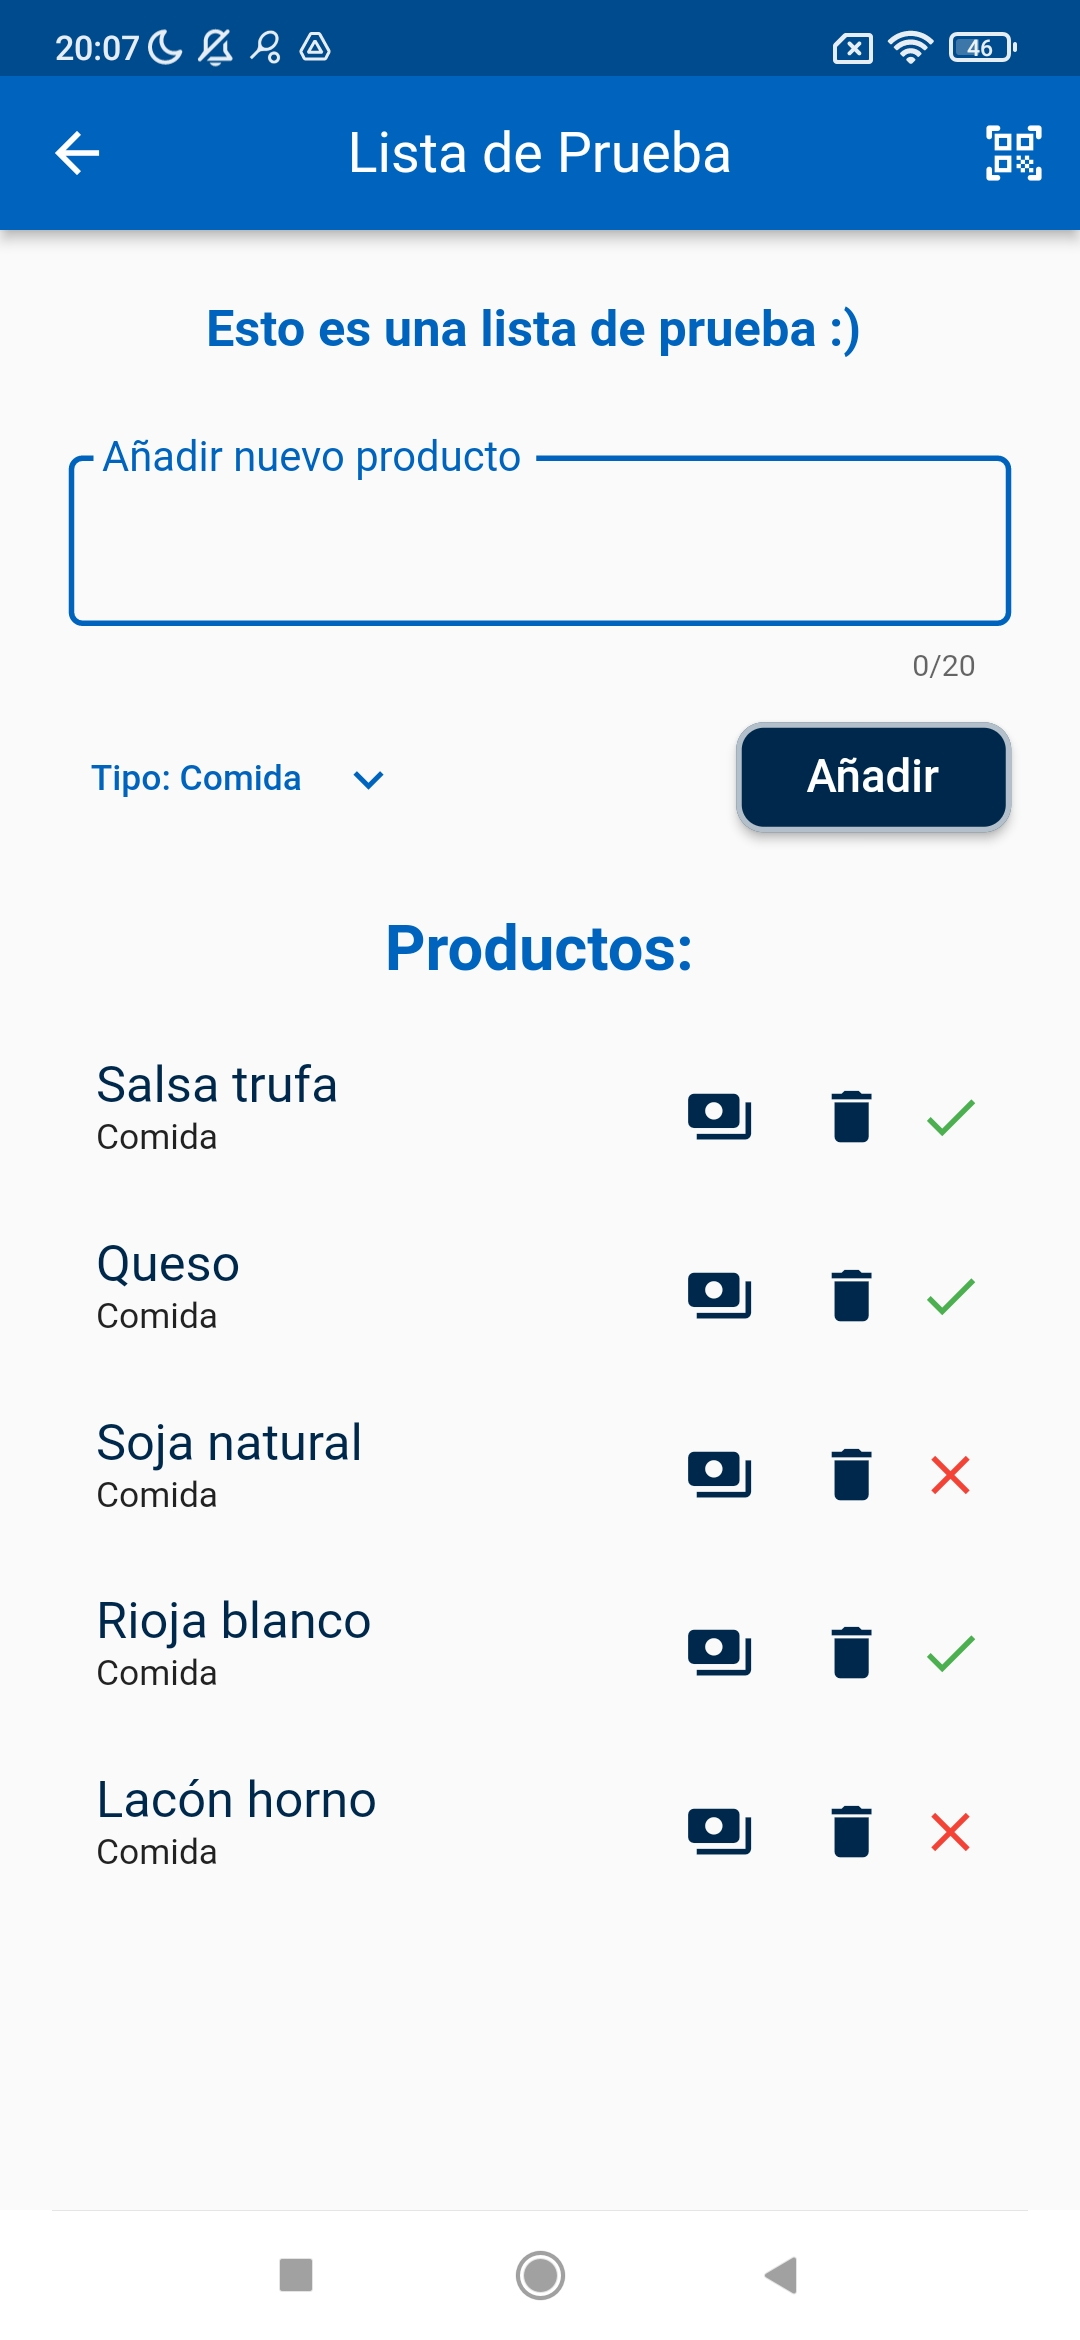
\includegraphics[width=\textwidth]{imagenes/pantallas/listas/detalles.jpg}
        \caption{Productos}
        \label{fig:productos}
    \end{minipage}
    \hspace{1cm}
    \begin{minipage}[h]{0.35\textwidth}
        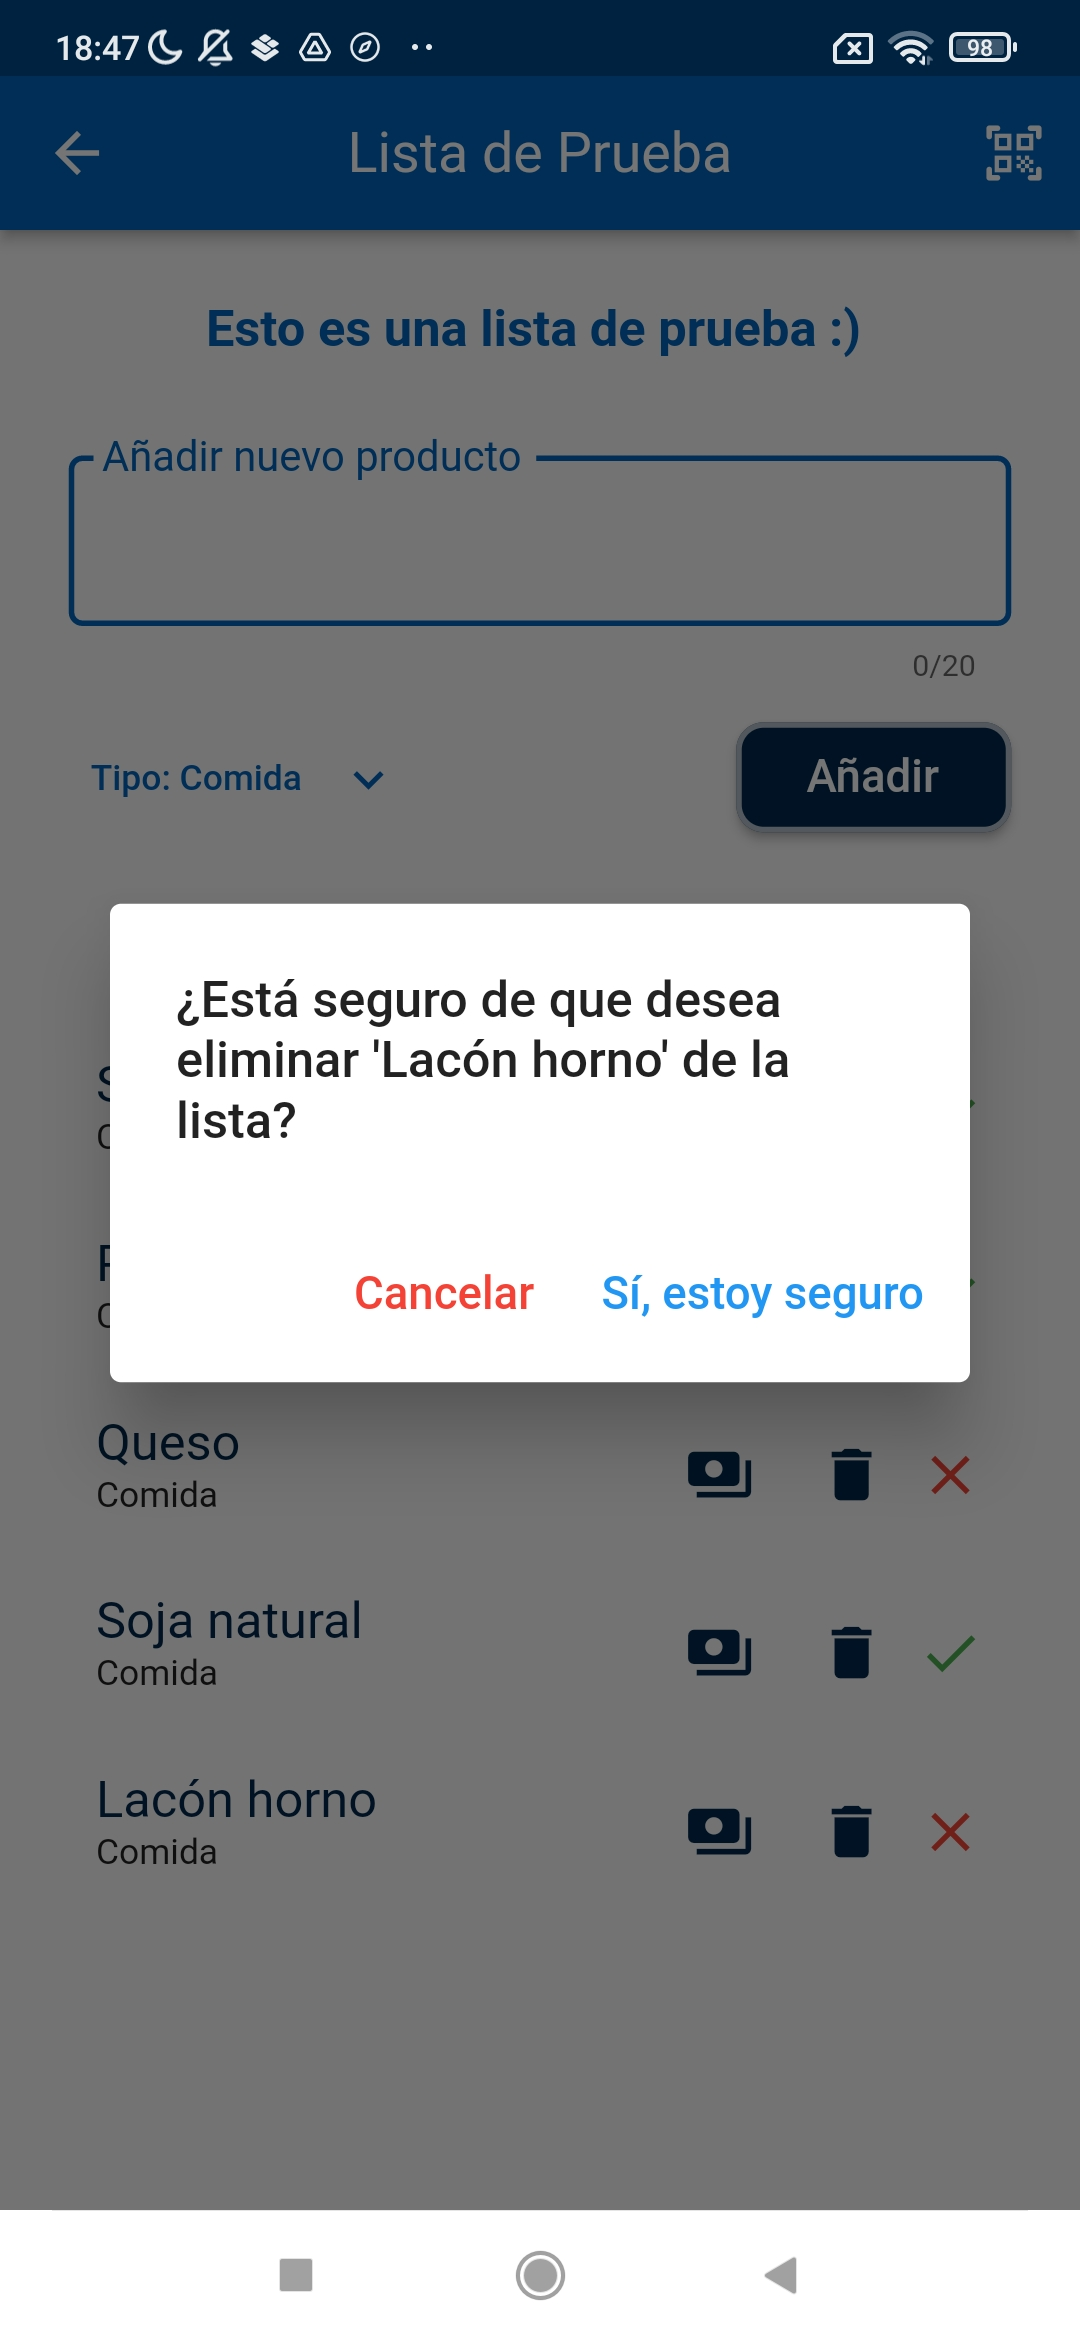
\includegraphics[width=\textwidth]{imagenes/pantallas/listas/modal_borrar_producto.jpg}
        \caption{Borrar un producto}
    \end{minipage}
\end{figure}

\subsection{Grupos}

Al seleccionar la pestaña correspondiente, se desplegará una nueva sección en la pantalla que mostrará el segundo gran bloque de la aplicación: los grupos. Esta sección contiene, desde la creación, edición y administración de grupos, como la funcionalidad de mensajería por chat de los mismos, además de permitir trabajar con listas grupales compartidas por los miembros de un mismo grupo.

\subsubsection{Visualización del listado de grupos}

La interfaz de usuario muestra un listado de chats, similar a la pantalla principal de las principales aplicaciones de mensajería. En la parte superior de la misma, el diseño de la interfaz de usuario es exactamente el mismo que el del listado de listas de la compra personales, pues comparten la misma cabecera.

La mayor parte de la pantalla se dedica al listado de chats. Al igual que en la obtención de las listas de la compra, se muestra inicialmente un círculo de carga, mientras se obtiene la información de la base de datos. En caso de no encontrar ningún grupo al que pertenezca el usuario, se mostrará un mensaje amigable indicando al usuario que se puede unir al grupo que desee o crear uno nuevo.  Por otro lado, si el usuario ya está asociado a uno o varios grupos, se mostrarán en pantalla todos los chats a los que tiene acceso, pudiendo fácilmente acceder a ellos con un simple click, de manera rápida y eficiente.

\newpage

Cada chat se representa como una fila individual en la lista, que contiene información relevante sobre la conversación. Para cada uno, se muestra la inicial del nombre del grupo a la izquierda, delimitada por un círculo azul que mantiene el estilo de colores de la aplicación, seguido del nombre del mismo.

\begin{wrapfigure}{l}{0.35\textwidth}
    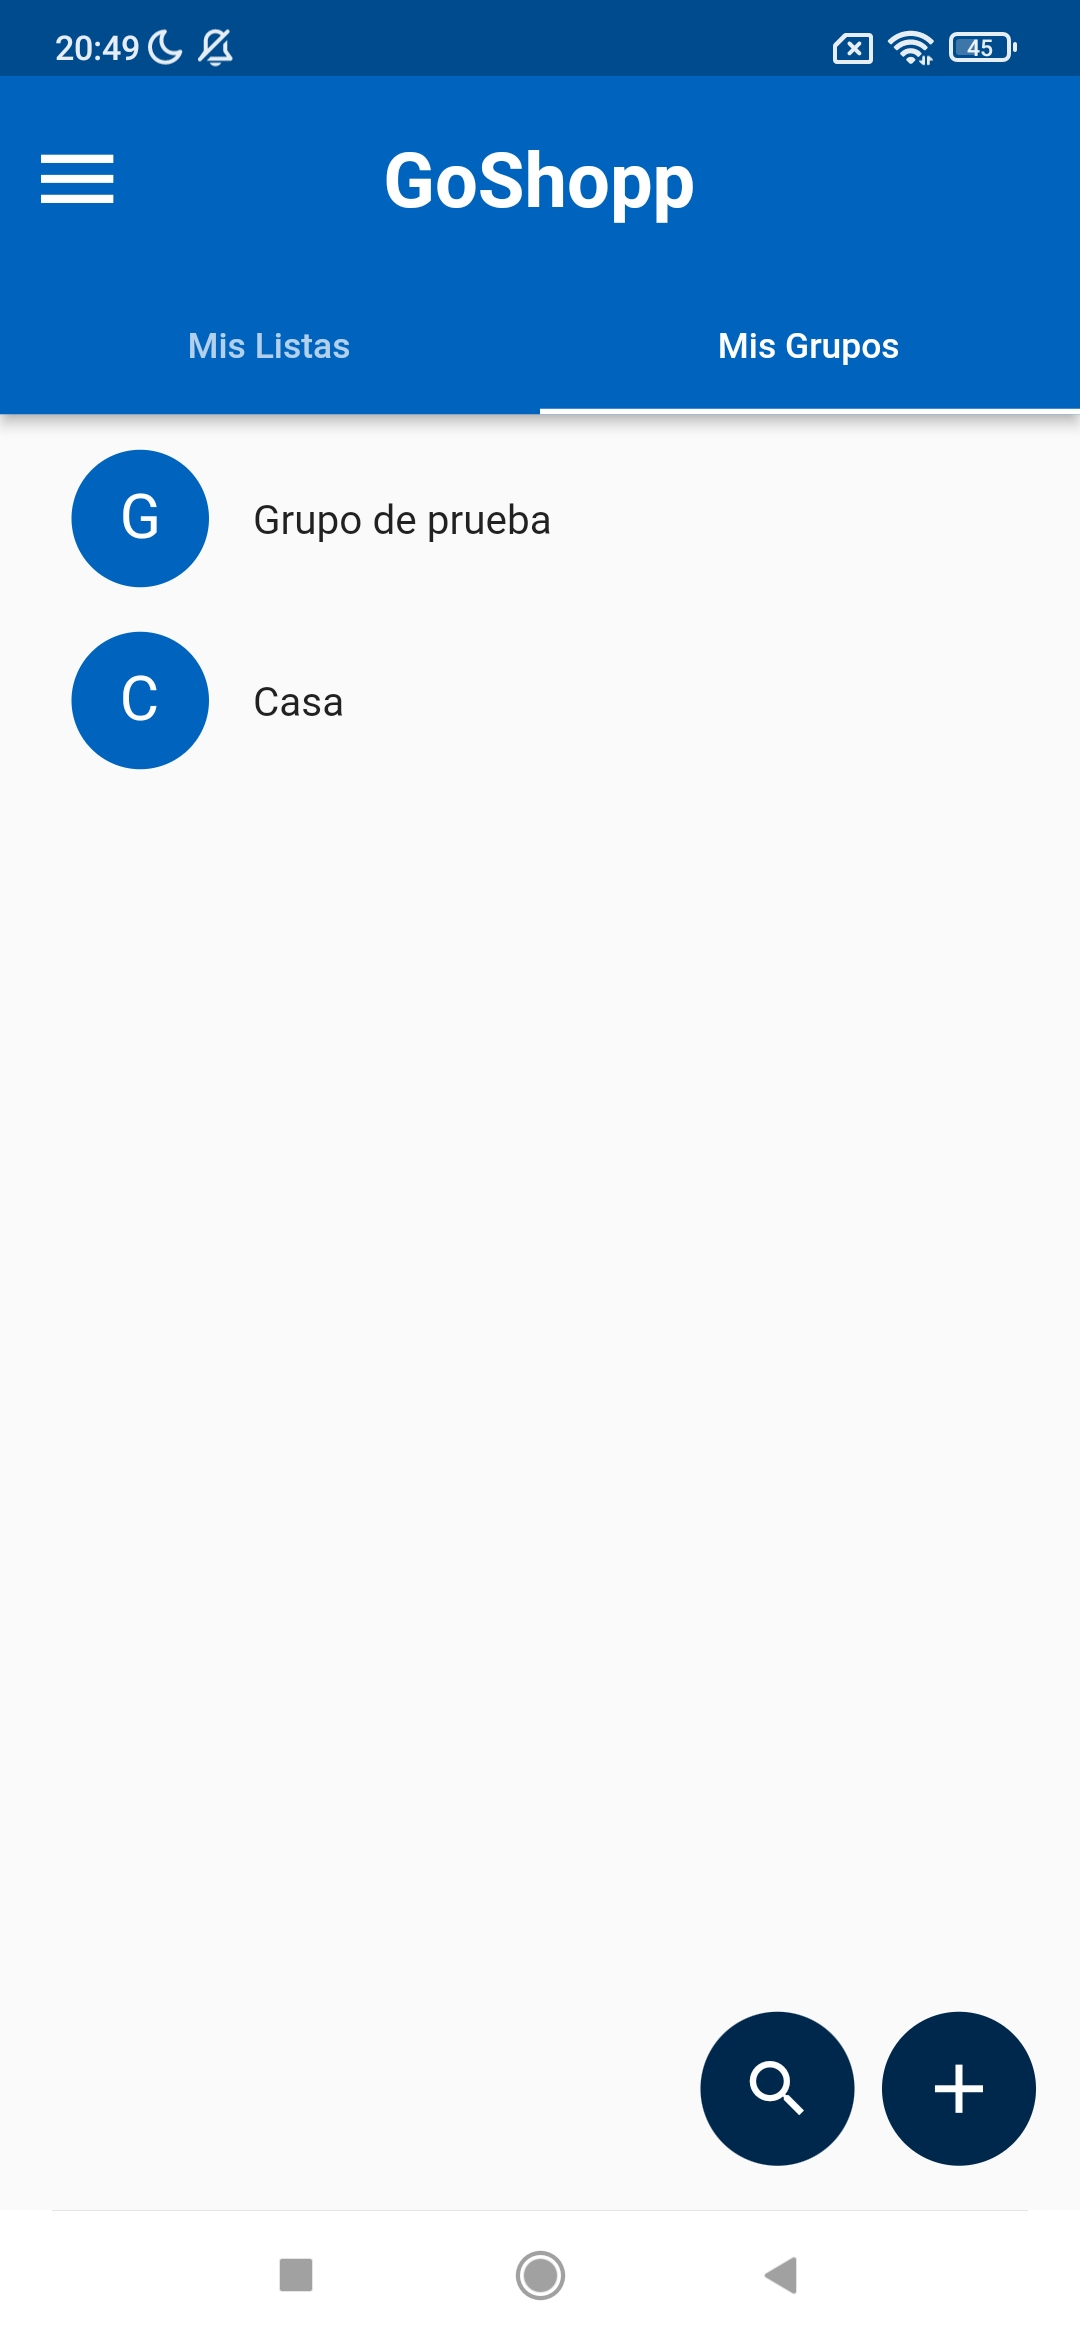
\includegraphics[width=0.32\textwidth]{imagenes/pantallas/grupos/grupos.jpg}
    \caption{Listado de grupos}
    \vspace{-5\intextsep}
\end{wrapfigure}

Al final de la pantalla, en la parte inferior, se incluyen iconos de acción para interactuar con la aplicación, tanto para crear grupos nuevos como para buscar uno ya existente. Estos iconos se representan en un color más oscuro, mediante un icono de una lupa y un símbolo de suma, respectivamente.

La interfaz de usuario está diseñada para facilitar la visualización y navegación entre los diferentes chats disponibles y proporciona una vista clara y organizada de las conversaciones, mostrando información relevante para identificar un grupo rápidamente. En general, esta interfaz de usuario busca ofrecer una experiencia intuitiva y eficiente para la gestión de las conversaciones, intentando asemejarse lo máximo posible el aspecto de una aplicación de mensajería.

\subsubsection{Crear un grupo nuevo}

Al pulsar sobre el botón utilizado para crear un nuevo grupo, se activa un modal que aparece en primer plano, superponiéndose a la pantalla principal. Este modal tiene como objetivo permitir al usuario introducir el nombre de un grupo. Dentro del modal, se encuentra un campo de texto donde el usuario puede ingresar el nombre deseado para el grupo.

Además, se incluyen dos botones en el modal. El primer botón, etiquetado como \textit{Cancelar} y en color rojo, permite al usuario cerrar el modal sin realizar ninguna acción, volviendo a la interfaz principal sin efectuar ningún cambio.

El segundo botón, etiquetado como \textit{Crear} y en color azul, tiene como objetivo confirmar la acción y crear el grupo con el nombre ingresado. Al pulsar este botón, se realiza el proceso de creación del grupo utilizando el nombre proporcionado en el campo de texto, mediante una inserción en la base de datos. Una vez creado el grupo, se muestra un mensaje indicando que el grupo se ha creado con éxito y el modal se cierra, redirigiendo al usuario a la pantalla de chat del nuevo grupo creado.

\subsubsection{Unirse a un grupo existente}

Si se pulsa sobre el botón representado mediante el icono de una lupa, se redirigirá al usuario a una nueva pestaña en la que se mostrará un buscador en la parte superior, diseñado para permitir la búsqueda de grupos específicos mediante su nombre. Junto al buscador, se encuentra un icono de lupa que sirve como botón para activar la búsqueda y obtener los resultados, los cuales se muestran en la misma pantalla, justo debajo del campo de texto.

Cada uno se presenta en una fila donde se muestra, al igual que en la pantalla principal, el nombre del grupo y la inicial del mismo, en negrita. Debajo del nombre del grupo, en caso de que el usuario no pertenezca al grupo en cuestión, se indica el administrador del mismo, lo que proporciona una referencia clara sobre quién es responsable de dicho grupo, evitando así equivocaciones en el caso de que aparezcan varios resultados con el mismo nombre.

Además, aparecerá un botón representado mediante una punta de flecha horizontal que permitirá al usuario unirse al grupo. Al pulsar en este botón, se le redirigirá a la pestaña de chat, obteniendo todos los mensajes existentes en el grupo y haciendo que el usuario forme parte del mismo. En caso de que el usuario ya pertenezca al grupo buscado, no se mostrará dicho botón de unirse y, en vez de la información acerca del administrador, aparecerá un mensaje: \textit{Ya formas parte de este grupo}.

\begin{figure}[h]
    \centering
    \begin{minipage}[h]{0.32\textwidth}
        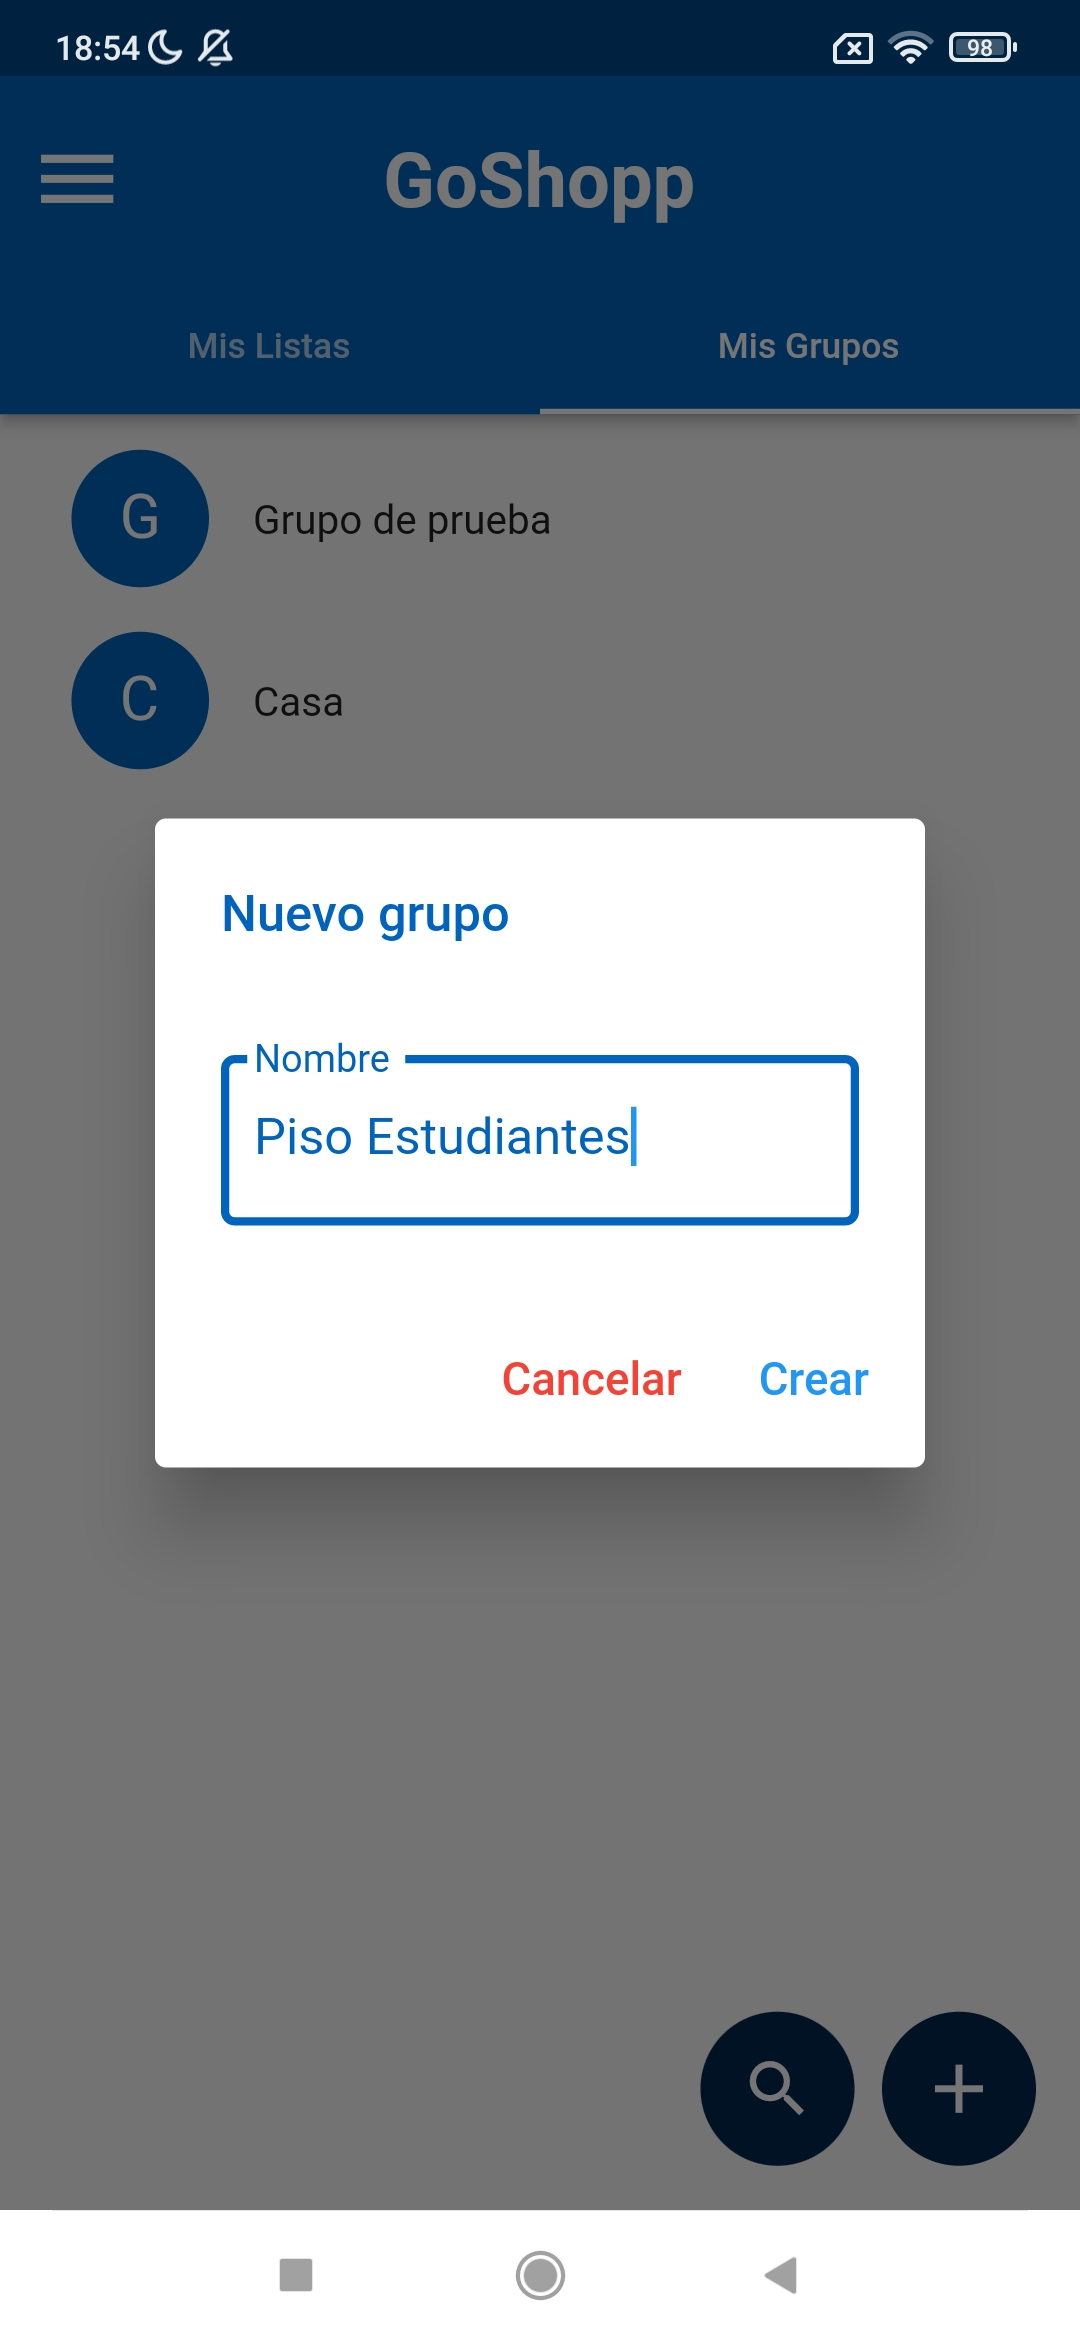
\includegraphics[width=\textwidth]{imagenes/pantallas/grupos/modal_crear_grupo.jpg}
        \caption{Crear un grupos}
    \end{minipage}
    \hspace{1cm}
    \begin{minipage}[h]{0.32\textwidth}
        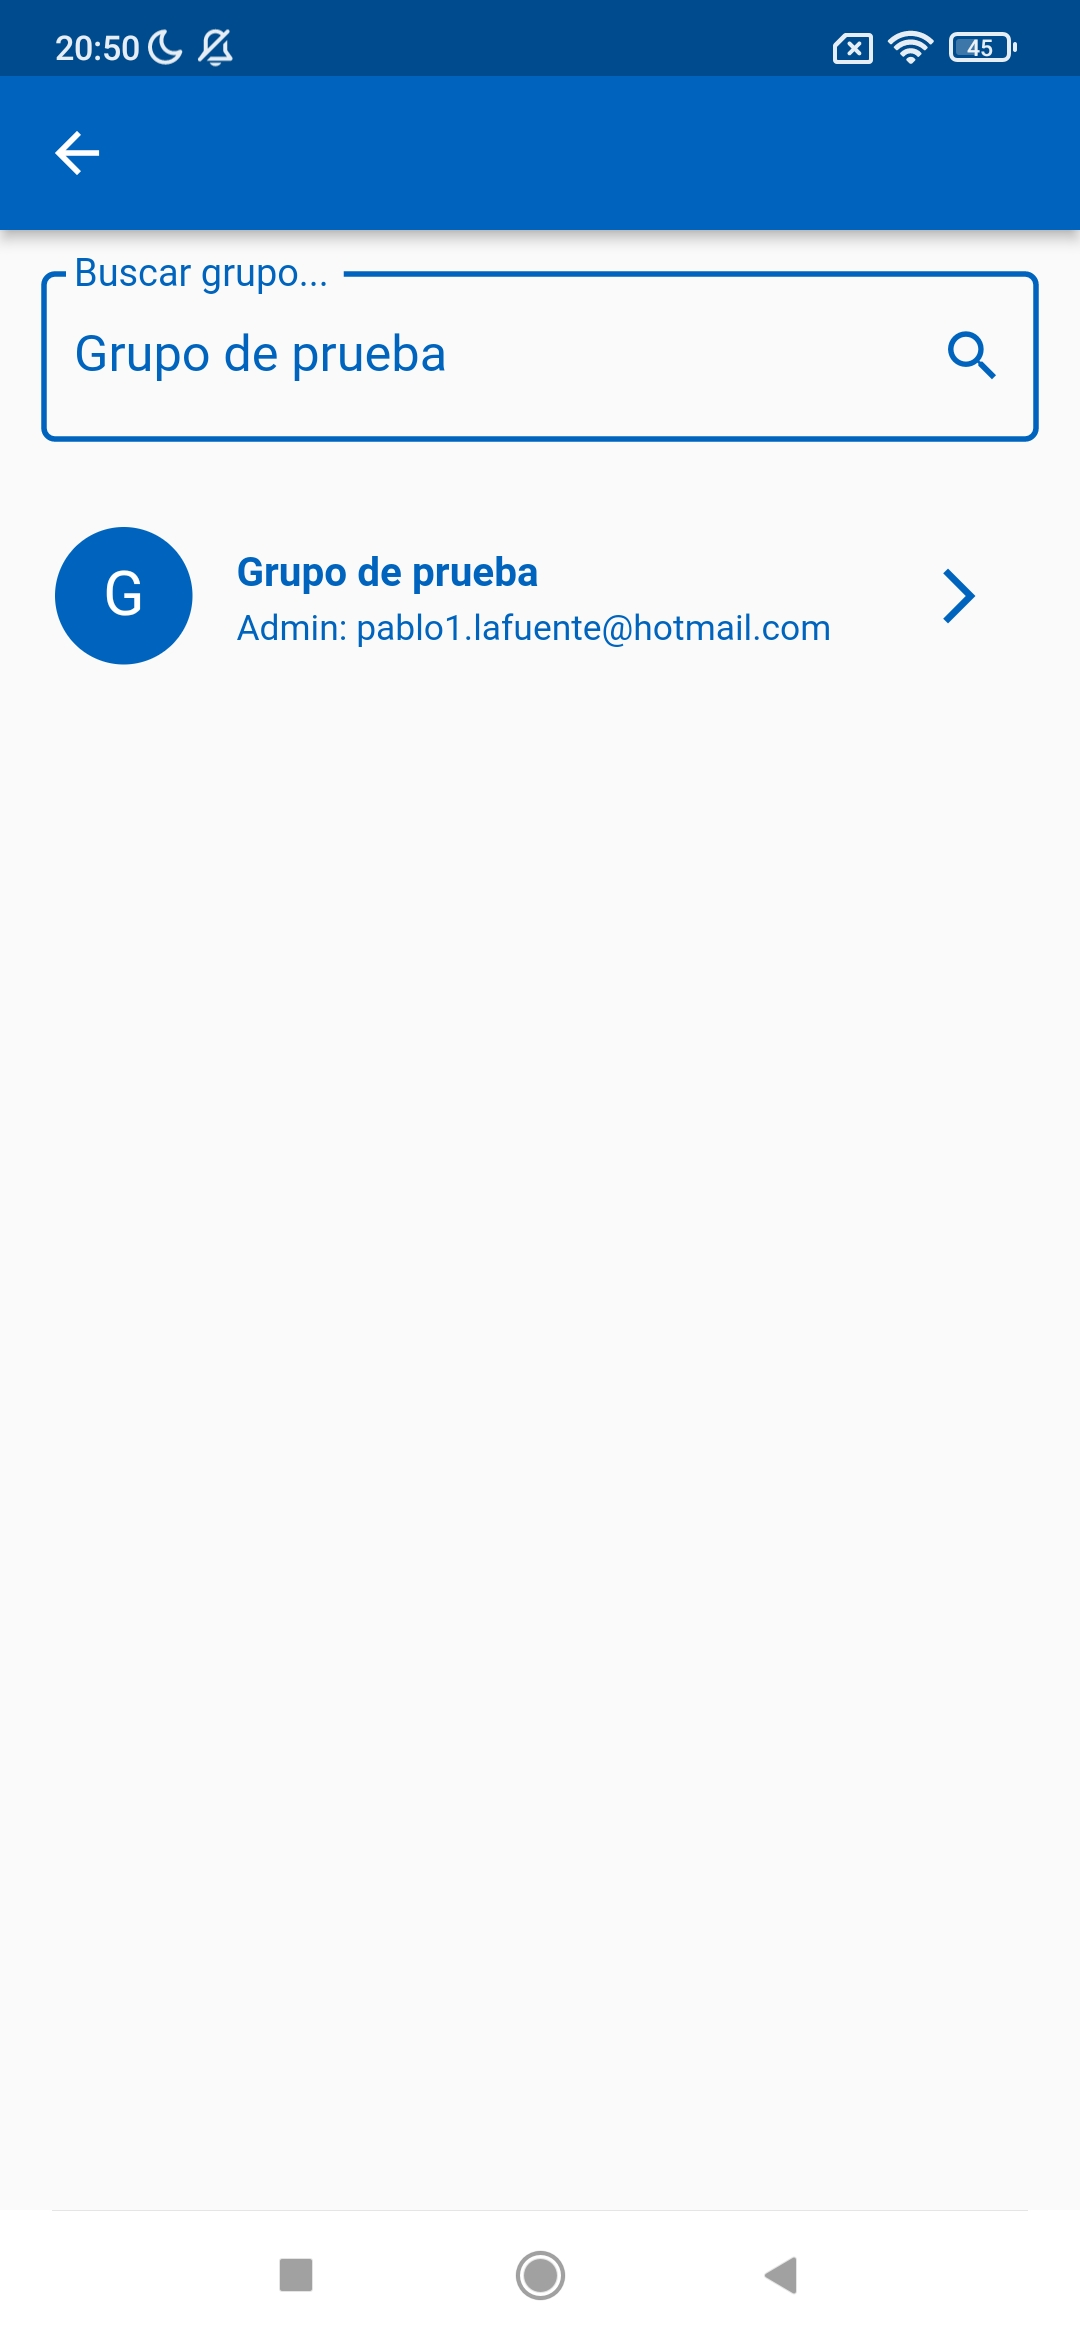
\includegraphics[width=\textwidth]{imagenes/pantallas/grupos/buscar_grupos.jpg}
        \caption{Buscador de grupos}
    \end{minipage}
\end{figure}

\subsubsection{Chat}

Ya sea pulsando en el chat correspondiente, uniéndose mediante el botón del buscador o creando un nuevo grupo, se accede a la interfaz del envío y recepción de mensajes. Para ello, se ha implementado una interfaz de chat clásica, como las presentes en plataformas de redes sociales como WhatsApp o Telegram, la cual destaca por su diseño intuitivo y su funcionalidad eficiente, que permite una comunicación fluida y cómoda entre los usuarios. A continuación, se describen con mayor detalle los elementos clave de esta interfaz, brindando una visión más completa de su estructura y características.

La pantalla principal de la interfaz de chat muestra una lista de mensajes que constituyen el historial completo de la conversación. Este diseño cronológico permite a los usuarios seguir fácilmente la secuencia de los intercambios de mensajes. Los mensajes más recientes se visualizan en la parte inferior de la pantalla y, a medida que la conversación avanza, los mensajes anteriores se desplazan hacia arriba, garantizando una experiencia de lectura coherente. Cada uno de los mensajes obtenidos de la base de datos, así como los nuevos insertados durante una conversación, se tratan como widgets independientes.

\newpage

Estos widgets, han sido diseñados para que se muestren de manera intuitiva, en forma de 'bocadillos' que aparecen desde la izquierda o derecha de la pantalla del dispositivo dependiendo quien sea el emisor del mensaje. Dentro de cada contenedor, se puede visualizar en la parte superior del mismo el nombre del emisor y la hora a la que se envió dicho mensaje, mientras que en la parte inferior se muestra el contenido del mismo.

Para facilitar la legibilidad y la comprensión de la conversación, se utiliza una disposición visualmente diferenciada para los mensajes del usuario y los mensajes de los demás participantes. De esta forma, los que han sido enviados por el usuario se alinean a la derecha de la pantalla, mientras que los mensajes de los demás integrantes del chat se sitúan a la izquierda. Esta distinción clara permite identificar rápidamente quién es el autor de cada mensaje y mejora la navegación visual dentro de la interfaz de chat.

\begin{wrapfigure}{l}{0.35\textwidth}
    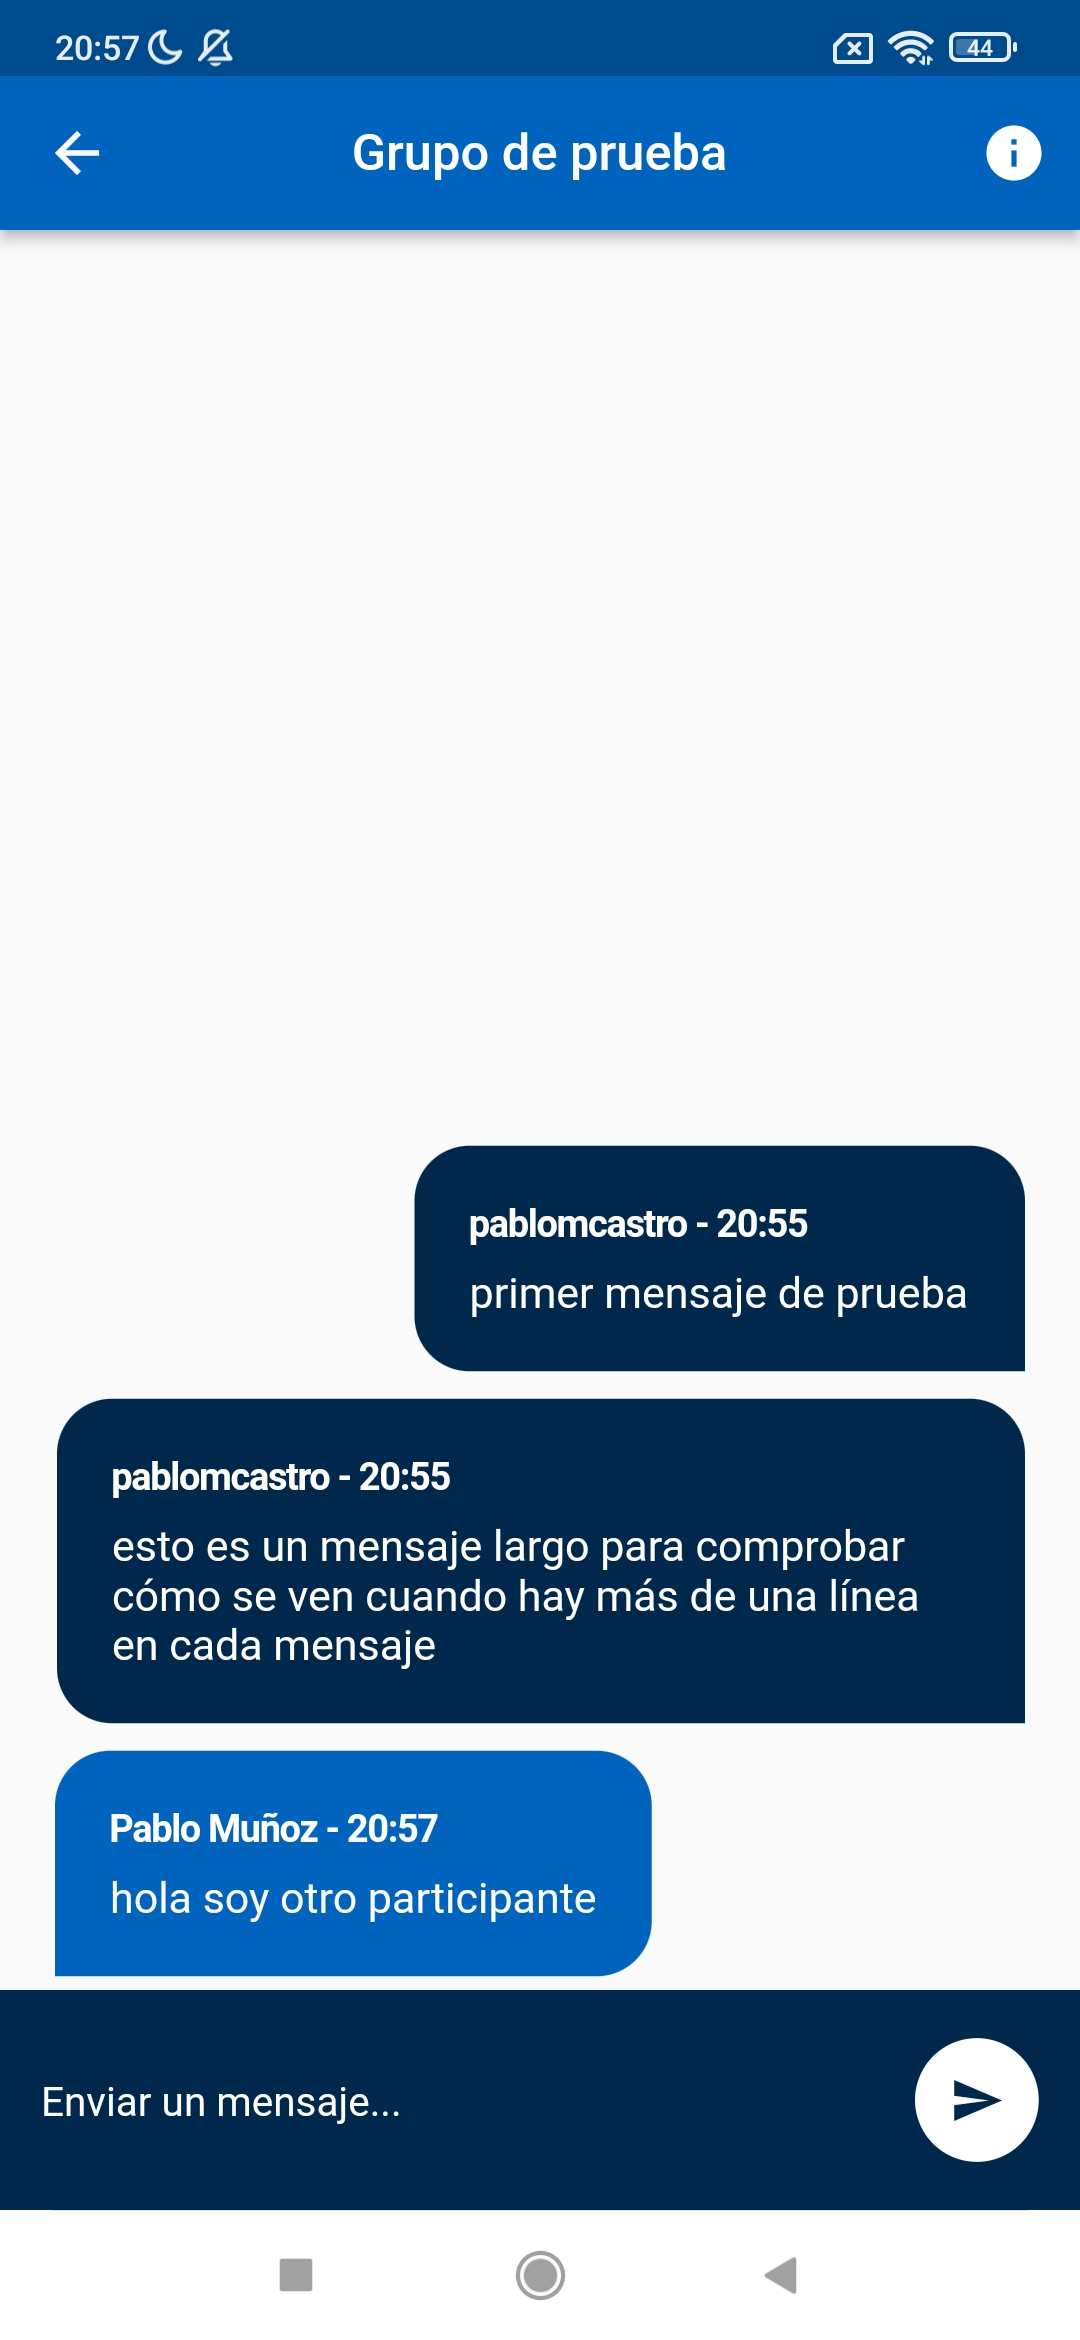
\includegraphics[width=0.32\textwidth]{imagenes/pantallas/grupos/chat.jpg}
    \caption{Interfaz del chat}
    \vspace{-4\intextsep}
\end{wrapfigure}

En la parte inferior de la pantalla, se encuentra la barra de texto, un componente fundamental para la interacción activa en el chat. Mediante esta barra de texto, los usuarios pueden redactar y enviar mensajes en tiempo real. Al escribir en la barra de texto y presionar el botón de envío, los mensajes se agregan a la conversación, siendo colocados en la parte más reciente de la lista de mensajes. Esto asegura que las contribuciones más recientes se presenten de manera prominente, manteniendo el hilo de la conversación de forma coherente.

La implementación de esta interfaz de chat clásica se centra en la simplicidad y la facilidad de uso, permitiendo a los usuarios comunicarse de manera efectiva. El diseño visual, con la disposición distinta de los mensajes del usuario y de los demás participantes, ayuda a una rápida identificación de los autores. Además, la barra de texto en la parte inferior ofrece una forma intuitiva y práctica de ingresar mensajes nuevos, facilitando una comunicación fluida en el chat. En conjunto, estos elementos crean una experiencia de chat cómoda y funcional para los usuarios.

\subsubsection{Información de un grupo}

Si se desea acceder a la información detallada de un grupo y explorar las listas de la compra asociadas al mismo, basta con pulsar el botón ubicado en la sección de chat, específicamente en la esquina superior derecha de la interfaz. Esto ofrece un enfoque intuitivo y accesible para los usuarios.

Al ingresar a la sección del grupo, se muestra un encabezado que resume la información principal del chat de grupo. Este encabezado incluye el nombre del grupo y el nombre de su administrador, acompañados de uno o dos botones dependiendo del perfil del usuario. Para los miembros regulares del grupo, se muestra únicamente el icono situado más a la izquierda, el cual permite a dichos usuarios abandonar el grupo si así lo desean, tras mostrar un mensaje de confirmación. Por otro lado, si el usuario es el administrador del grupo, se le proporciona un segundo botón adicional que le permite eliminar el grupo por completo, eliminando así toda la información asociada y expulsando a todos los usuarios.

Seguidamente, se encuentra una sección específica titulada \textit{Ver listas...} donde se presenta un listado de todas las listas de la compra pertenecientes al grupo. El formato utilizado en esta sección sigue la misma estructura y presentación visual que se emplea en las listas de la compra personales.

\newpage

Esta disposición uniforme y familiar permite a todos los miembros del grupo acceder rápidamente a la información relacionada con las listas y les ofrece la posibilidad de crear, editar o eliminar listas de forma ágil y cómoda.

Finalmente, se muestra un listado de los usuarios que forman parte del grupo, presentado en el orden cronológico de su incorporación al mismo. El administrador del grupo ocupa el primer lugar en esta lista, ya que, como se mencionó anteriormente, la jerarquía de administración se establece de tal manera que el usuario que lleva más tiempo siendo miembro del grupo se convierte en el administrador.

La implementación de esta interfaz de usuario prioriza la accesibilidad y la facilidad de uso. La inspiración tomada de aplicaciones exitosas como Whatsapp garantiza una experiencia intuitiva y familiar para los usuarios. Además, se han incorporado características específicas para el manejo de grupos, como la visualización de listas de compra asociadas y la gestión de miembros y administradores. En conjunto, estas características permiten una interacción efectiva y cómoda con los grupos y sus respectivas funcionalidades.

\begin{figure}[h]
    \centering
    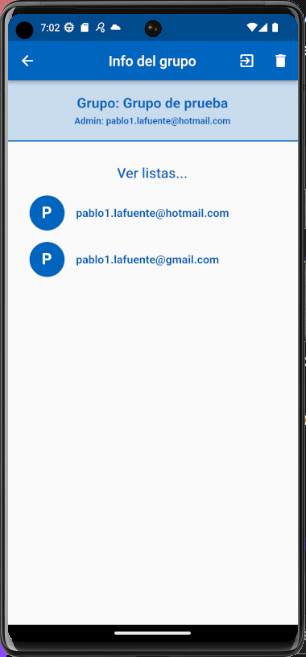
\includegraphics[width=0.32\textwidth]{imagenes/pantallas/grupos/info_grupo.png}
    \caption{Información del grupo}
\end{figure}

\subsection{Ejemplo real de escaneo de tickets de la compra}

Una vez mostrado todo el potencial de la aplicación, se presentarán una serie de ejemplos de escaneos de tickets de compra, acompañados de sus correspondientes resultados. Esta recopilación tiene como objetivo analizar y evaluar la efectividad de la funcionalidad implementada para la digitalización y procesamiento de información contenida en tickets de compra. 
A través de esta muestra de casos, se busca brindar una visión clara y precisa sobre la capacidad de dicha funcionalidad para extraer, interpretar y organizar los distintos productos reflejados en el ticket, de manera eficiente y precisa. Mediante el análisis detallado de los resultados obtenidos, se espera ofrecer una visión integral de las ventajas y limitaciones que esta tecnología presenta, así como posibles áreas de mejora para futuros desarrollos en este campo.

\begin{figure}[h]
    \centering
    \begin{minipage}[h]{0.32\textwidth}
        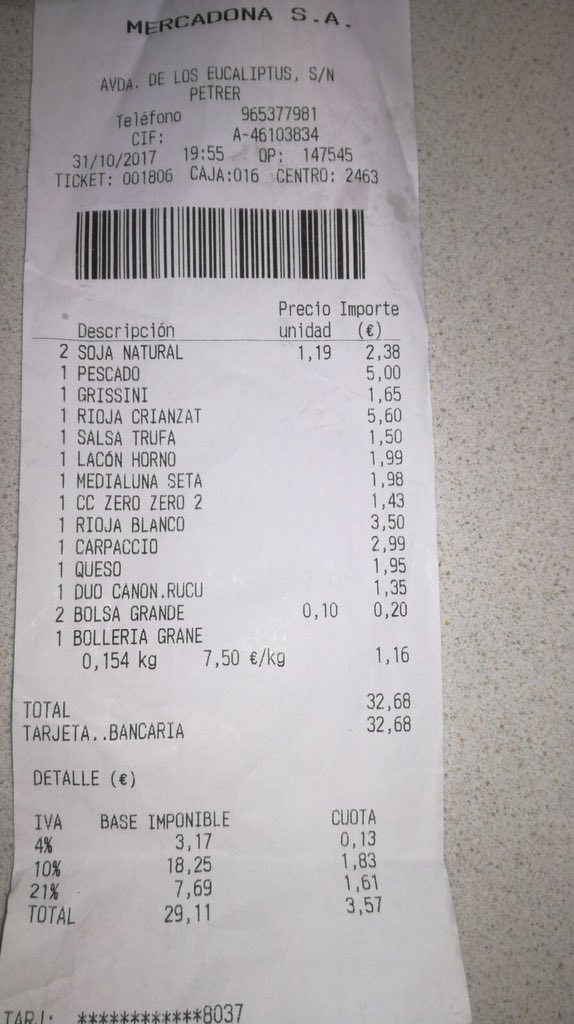
\includegraphics[width=\textwidth]{imagenes/funcionamiento/ticket1.jpg}
        \caption{Ticket de Mercadona}
    \end{minipage}
    \hfill
    \begin{minipage}[h]{0.32\textwidth}
        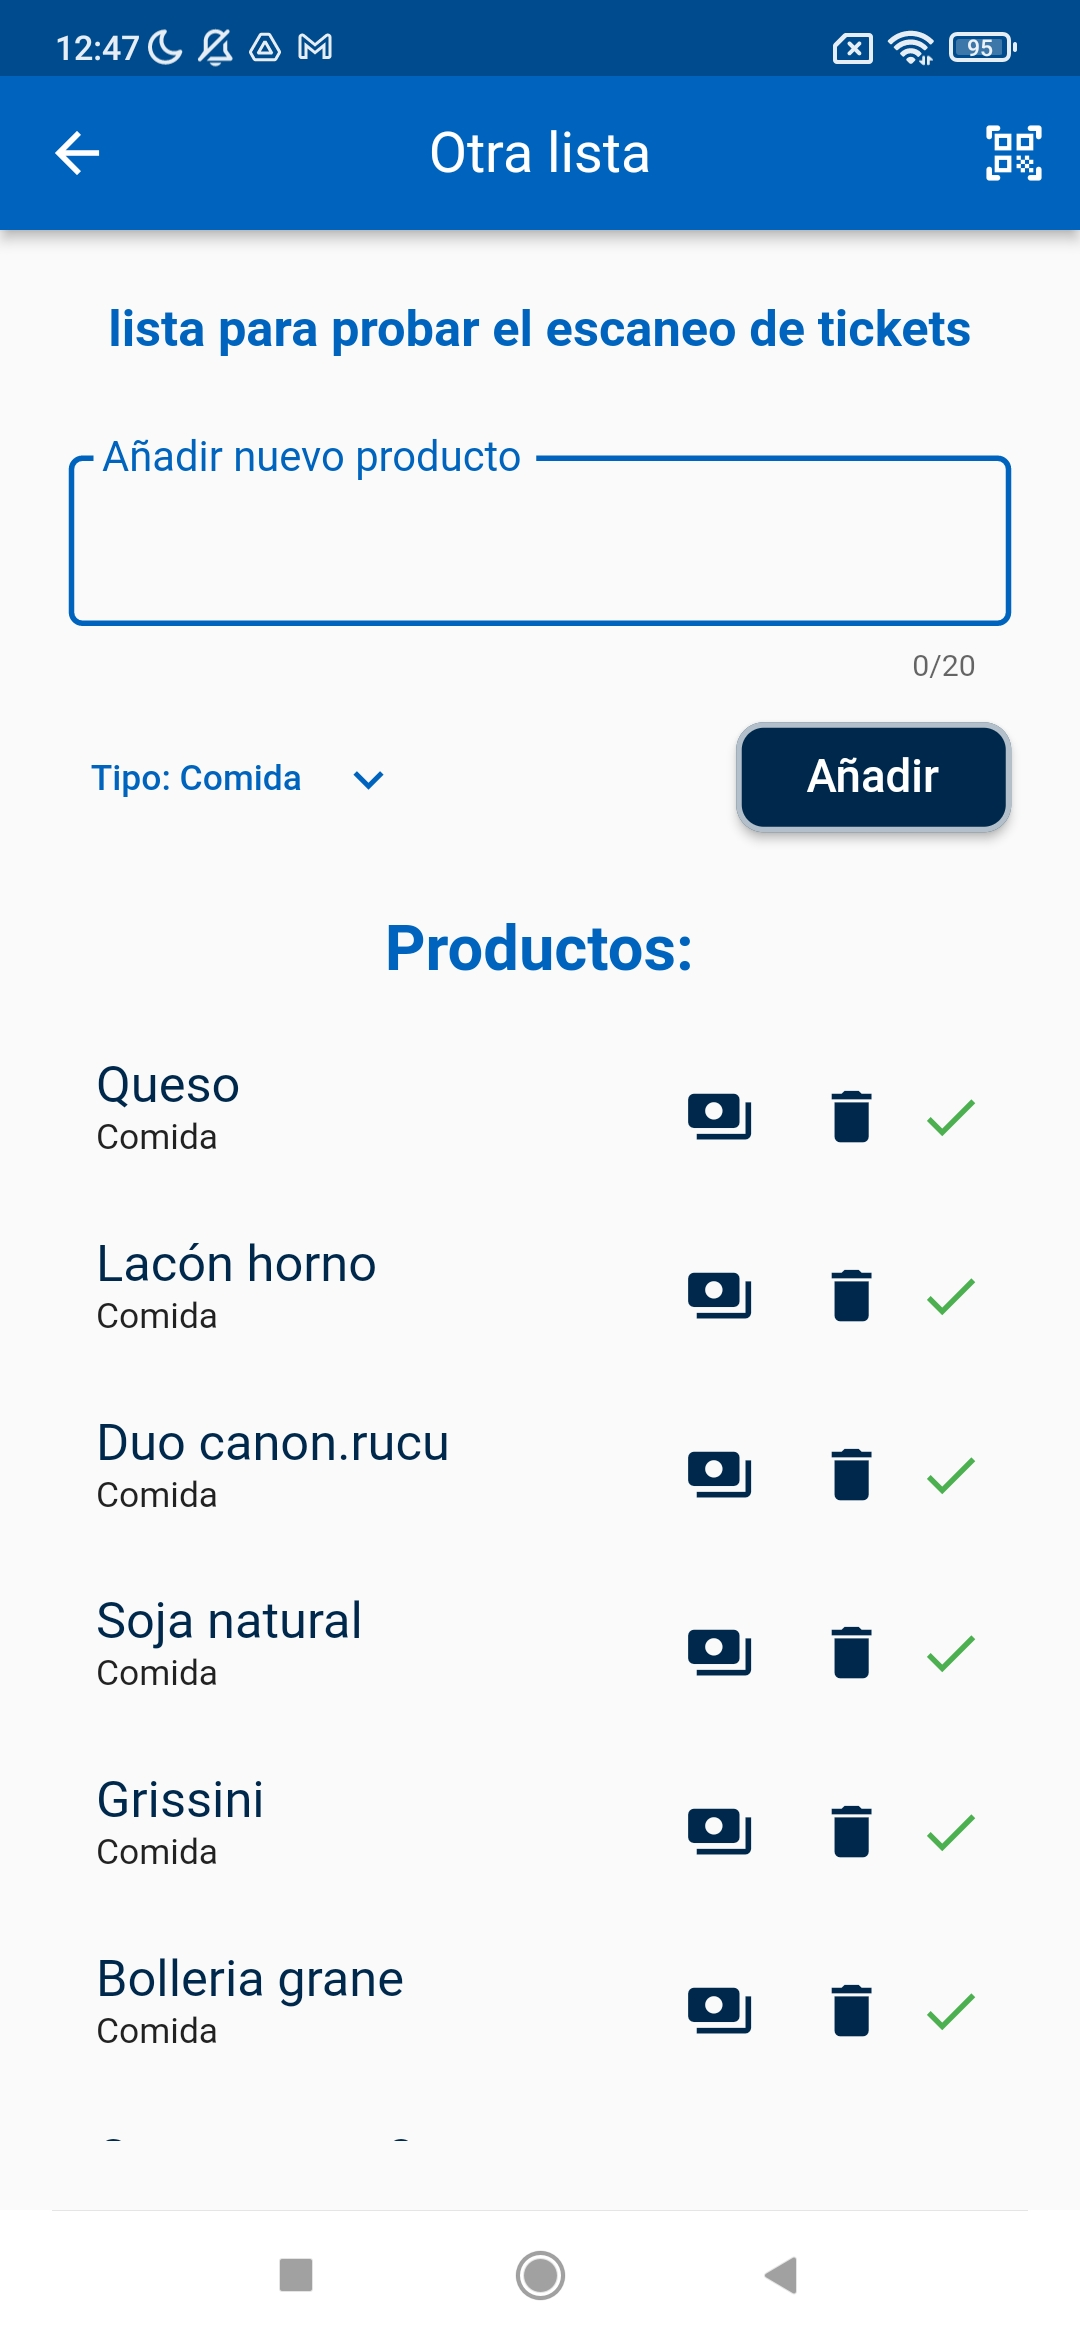
\includegraphics[width=\textwidth]{imagenes/funcionamiento/ticket1_res1.jpg}
        \caption{Resultado del escaneo: visualización 1}
    \end{minipage}
    \begin{minipage}[h]{0.32\textwidth}
        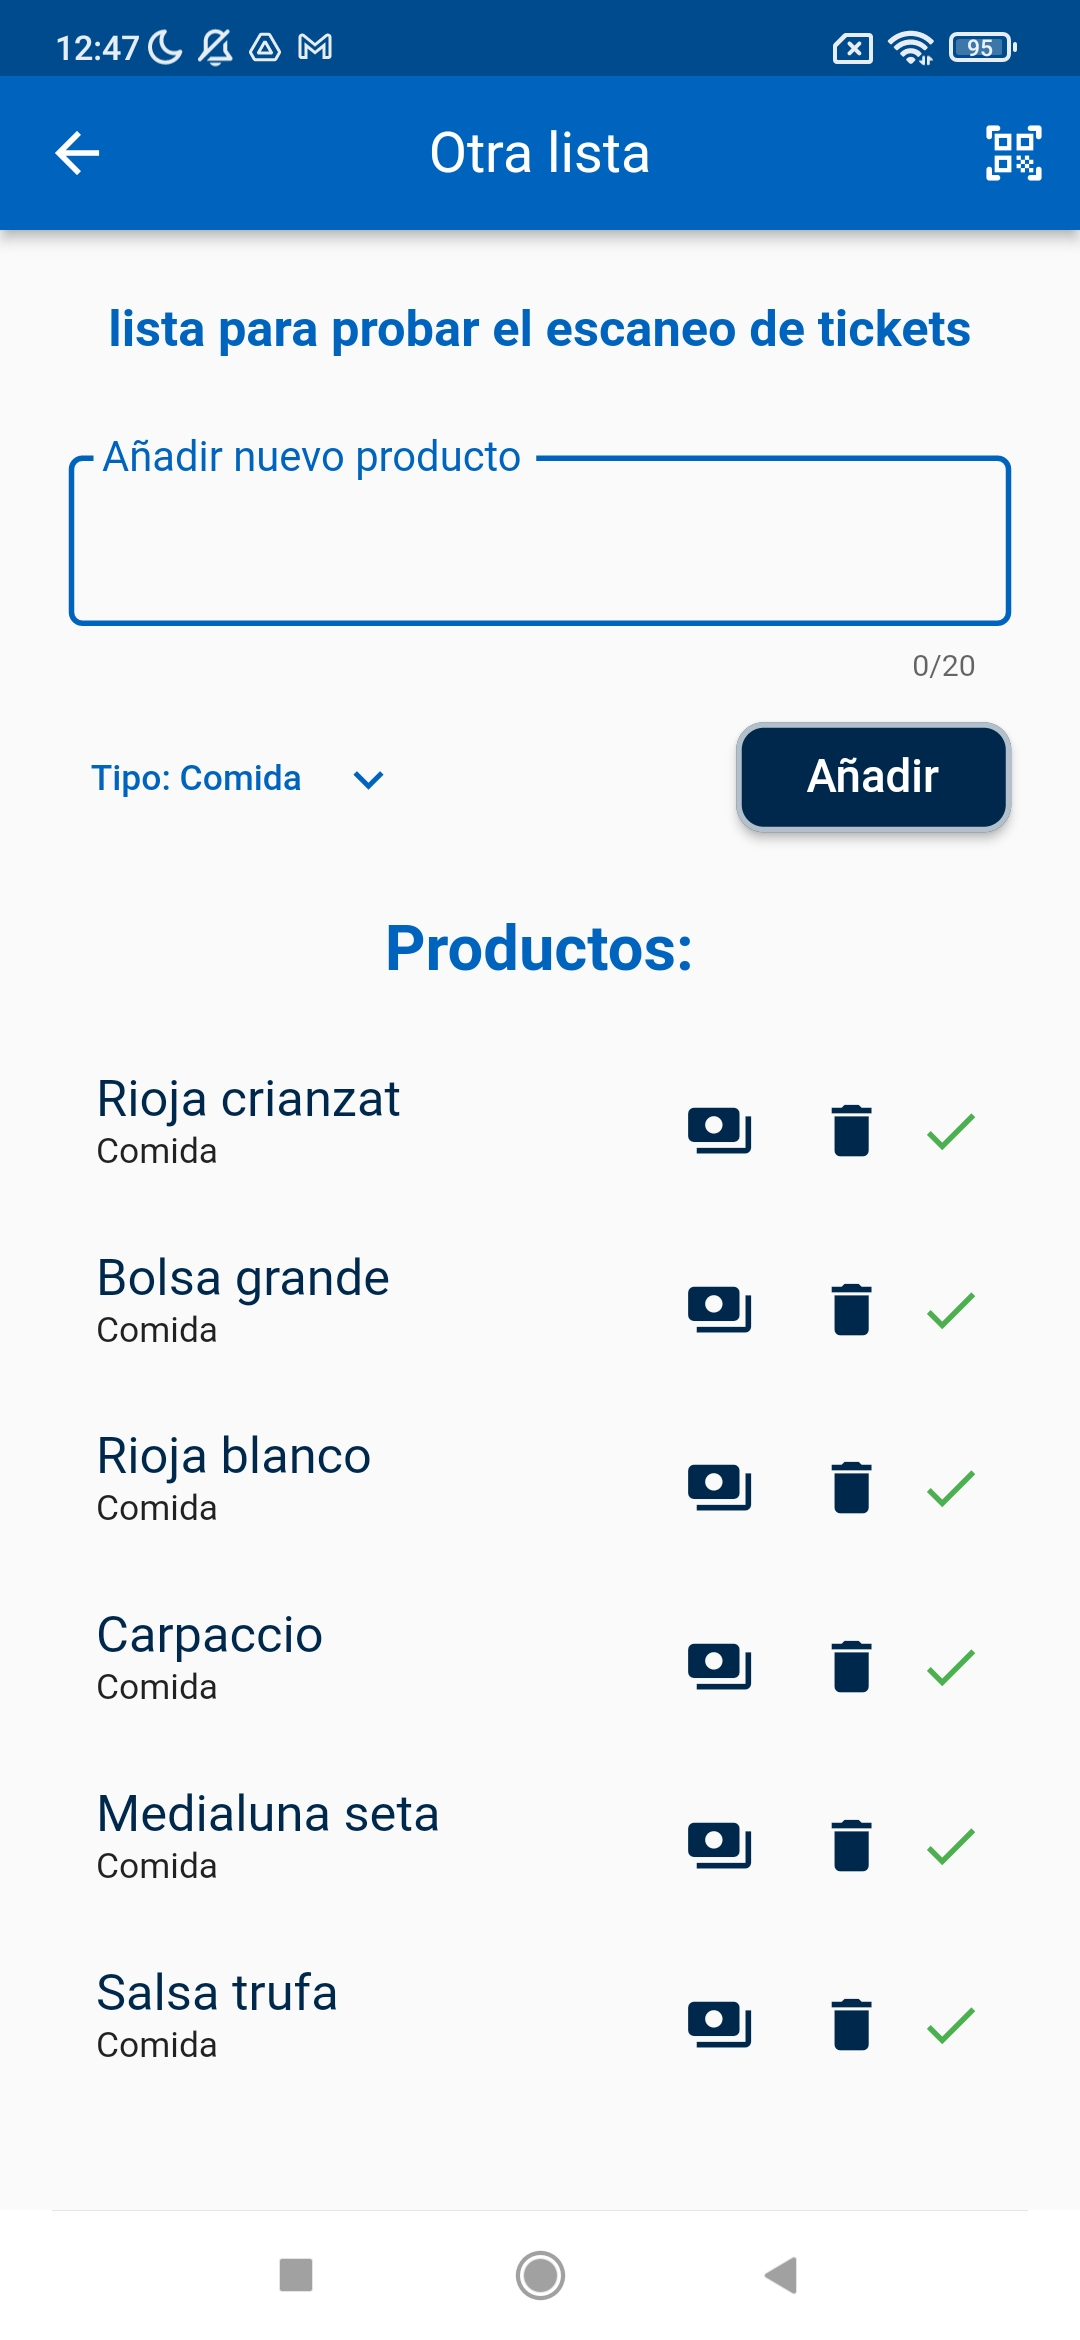
\includegraphics[width=\textwidth]{imagenes/funcionamiento/ticket1_res2.jpg}
        \caption{Resultado del escaneo: visualización 2}
    \end{minipage}
\end{figure}

En el ejemplo anterior, se puede ver claramente el funcionamiento de dicha funcionalidad. En primer lugar, se presenta la imagen del ticket de compra, el cual pertenece a una cadena de supermercados muy conocida como es Mercadona. Esta imagen sirve como punto de partida para nuestro proceso de escaneo y extracción de información relevante.

Posteriormente, se exhibe una fotografía que muestra el resultado del escaneo realizado por nuestro sistema. En esta imagen, se puede apreciar claramente la aplicación únicamente se ha quedado con los nombres de los productos, los cuales han sido reconocidos y extraídos de manera precisa, pues no falta ninguno. Además, se ha verificado que cada uno de estos elementos ha sido correctamente agregado a la lista correspondiente, lo cual se puede demostrar viendo que todos siguen el mismo diseño, pues se han creado widgets independientes para cada uno de ellos.

En este caso se muestran dos capturas de pantalla de la aplicación, pues el contenido del ticket es muy largo, lo cual demuestra también que la aplicación está preparada para cualquier cantidad de productos que se quieran añadir a una lista. De esta forma, y situándonos en la primera captura de pantalla, solo se tiene que deslizar de manera vertical sobre los productos para obtener la última imagen y poder visualizarlos todos.

Con base en estos resultados, podemos concluir de manera concluyente que nuestro sistema de escaneo de tickets de compra ha demostrado una notable capacidad para reconocer y agregar de manera precisa todos los productos a una lista correspondiente. Sin embargo, y como se explicará posteriormente, no todos los tipos de tickets son susceptibles de poder ser escaneados por nuestra aplicación, pues no todos los supermercados y tiendas tienen el mismo formato a la hora de mostrar los tickets de la compra.

\subsection{Extras}

Con el objetivo de brindar funcionalidades adicionales y acercar nuestra aplicación al usuario, hemos incorporado un elemento destacado en la pantalla principal donde se visualizan las listas personales y los grupos. En la esquina superior izquierda, se encuentra un icono de menú que proporciona acceso a una barra lateral con información relevante y personalizada.

Al hacer clic en el icono de menú, se desplegará una barra lateral que presenta datos clave del usuario. En primer lugar, se mostrará el nombre de usuario, permitiendo a los usuarios identificarse fácilmente y personalizar su experiencia en la aplicación. Además, si el usuario ha configurado una imagen de perfil, esta se exhibirá junto a su nombre, proporcionando un toque visual distintivo y familiar. En caso de que el usuario no haya seleccionado una imagen de perfil, se mostrará la inicial del nombre de usuario como una alternativa elegante y minimalista.

La inclusión de esta barra lateral y la visualización del nombre de usuario y, si está disponible, la imagen de perfil, enriquece la interfaz de usuario al brindar una sensación de pertenencia y personalización. Esto permite a los usuarios identificarse fácilmente y sentirse más conectados con su cuenta personal. Además, esta funcionalidad se suma al objetivo de ofrecer una experiencia intuitiva y agradable en nuestra aplicación, donde cada detalle se ha cuidado para garantizar la comodidad y satisfacción del usuario.

\subsubsection{Editar perfil de usuario}

Justo debajo del icono de menú, nos encontramos con tres botones que ofrecen funcionalidades adicionales. El primer botón, claramente identificado, nos permite acceder a una ventana dedicada a la modificación de los datos de perfil. Al hacer clic en este botón, se abrirá una nueva ventana que presenta una serie de elementos diseñados para facilitar la personalización del perfil del usuario.

En primer lugar, se muestra un área destinada a exhibir la imagen de perfil actual del usuario. Al hacer clic en esta imagen, se abrirá la galería de imágenes del dispositivo, lo que permitirá al usuario seleccionar una nueva imagen de perfil de su elección. Esta funcionalidad brinda flexibilidad y opciones al usuario para reflejar su identidad y personalidad en la aplicación. Además, se ha incorporado un botón denominado \textit{Guardar imagen}, que tiene como objetivo permitir al usuario guardar la imagen de perfil seleccionada y aplicar los cambios realizados de manera rápida y sencilla.

En la misma ventana, se incluye un campo de texto editable que permite al usuario modificar su nombre de usuario, ofreciéndole la flexibilidad de cambiar el nombre de usuario según sus preferencias personales. Por último, se presenta un botón denominado \textit{Guardar} que cumple la función de guardar el nombre de usuario modificado. Al hacer clic en este botón, los cambios realizados se guardarán de manera efectiva y se reflejarán en el perfil del usuario.

La implementación de esta ventana de modificación de datos de perfil busca ofrecer a los usuarios la posibilidad de personalizar su experiencia en la aplicación de acuerdo con sus preferencias individuales. La inclusión de elementos como la selección de imagen de perfil, la edición del nombre de usuario y los botones de guardado, permiten un proceso sencillo y práctico para realizar cambios en el perfil del usuario. Con estas funcionalidades, nos esforzamos por brindar a nuestros usuarios una aplicación adaptable y centrada en sus necesidades y preferencias personales.

\subsubsection{Sobre nosotros}

El segundo botón da paso a una ventana informativa que brinda detalles esenciales sobre la aplicación. Al hacer clic en este botón, se abrirá una nueva ventana donde se exhibe el logo distintivo de la misma, lo que proporciona una identificación visual clara y reconocible para los usuarios.

En esta ventana, también encontraremos una cuidadosa descripción de la aplicación que ha sido elaborada meticulosamente. Esta descripción incluye elementos clave que permiten a los usuarios comprender de manera concisa y precisa la esencia de la aplicación, así como su propósito y valor. Además, se hace mención explícita al nombre del autor, en este caso, el responsable de la creación y desarrollo de la aplicación.

La descripción proporcionada en esta ventana tiene como objetivo destacar las características principales y la funcionalidad destacada de la aplicación, brindando una visión general y clara de lo que los usuarios pueden esperar al utilizarla. Se enfatizan los beneficios y ventajas que la aplicación ofrece, destacando su utilidad y la forma en que puede mejorar la experiencia del usuario en el contexto específico para el cual ha sido diseñada.

Además, el tener este apartado puede ofrecer en un futuro la posibilidad de incluir de nueva información más detallada, noticias, novedades e incluso redes sociales o páginas externas para dar aún más posibilidad de crecimiento a la aplicación.

\begin{figure}[htbp]
    \centering
    \begin{minipage}[h]{0.32\textwidth}
        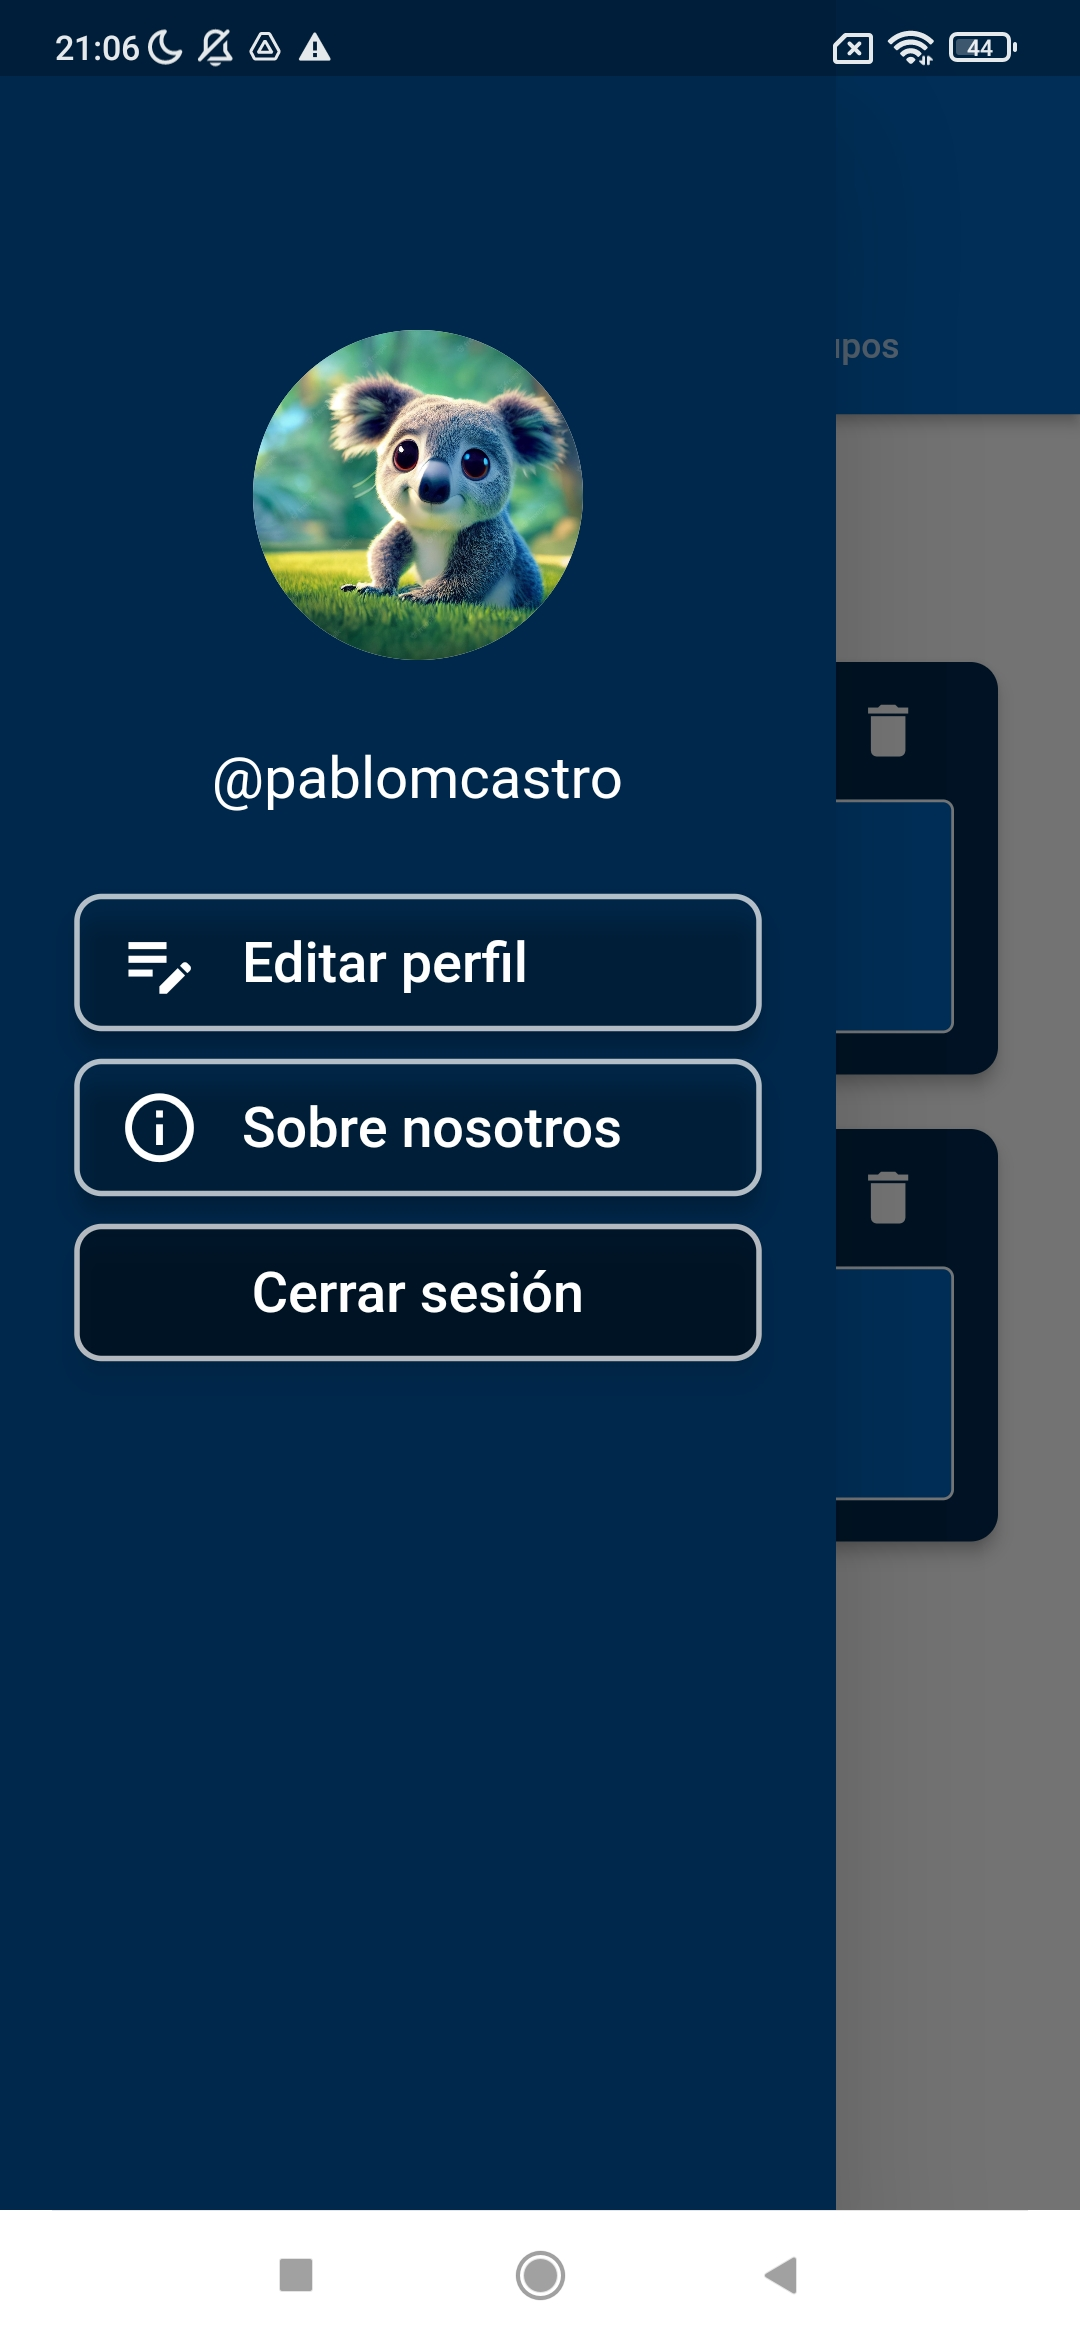
\includegraphics[width=\textwidth]{imagenes/pantallas/sidenav.jpg}
        \caption{Barra lateral}
    \end{minipage}
    \hfill    
    \begin{minipage}[h]{0.32\textwidth}
        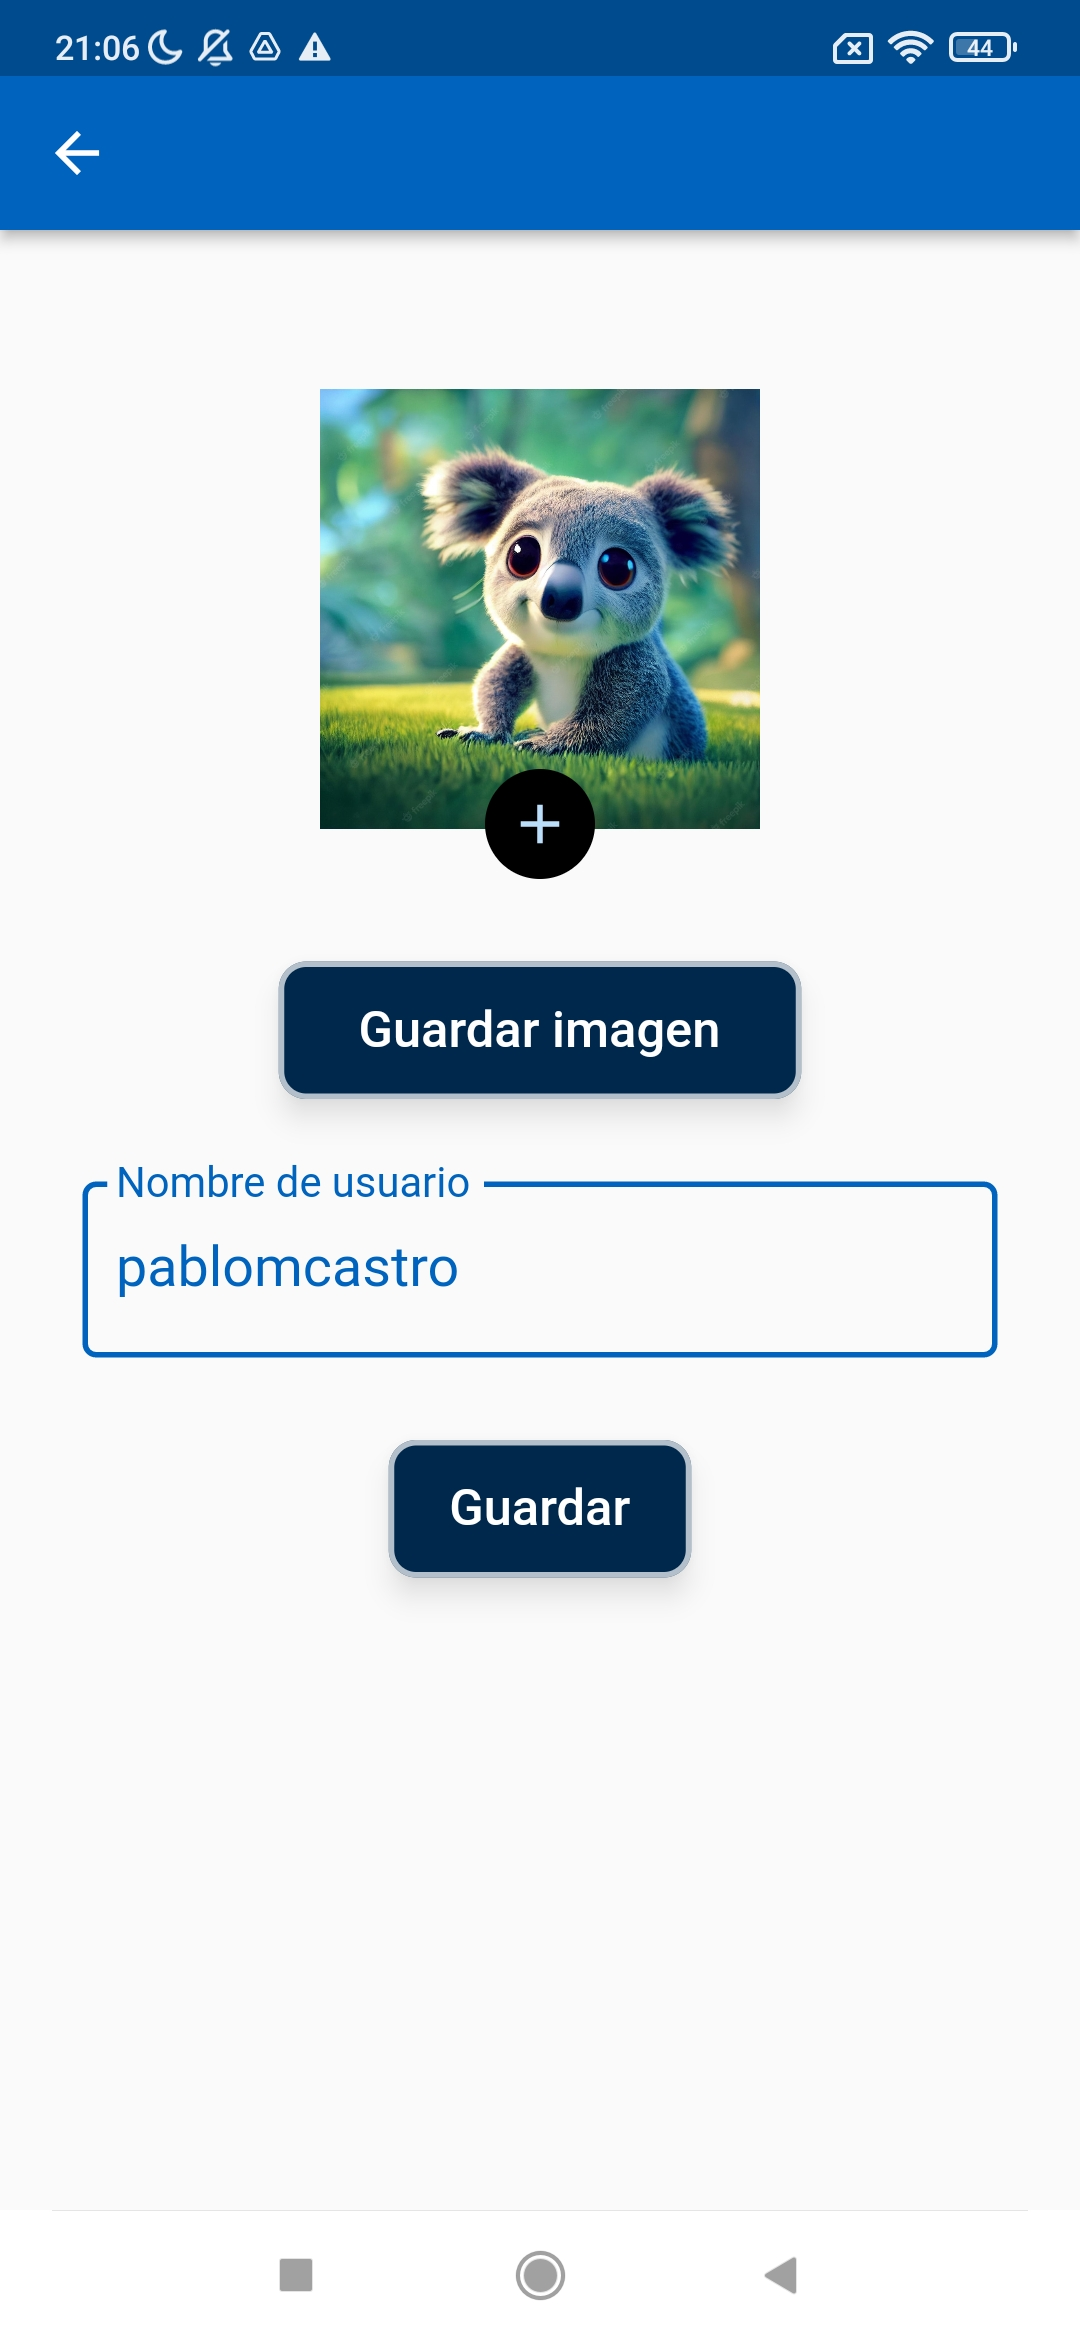
\includegraphics[width=\textwidth]{imagenes/pantallas/editar_perfil.jpg}
        \caption{Editar perfil}
    \end{minipage}
    \hfill
    \begin{minipage}[h]{0.32\textwidth}
        
\includegraphics[width=\textwidth]{imagenes/pantallas/info.jpg}
        \caption{Sobre nosotros}
    \end{minipage}
\end{figure}

\subsubsection{Cerrar la sesión del usuario}

En la parte inferior de la barra lateral del menú, se encuentra el tercer botón, cuya funcionalidad se centra en proporcionar al usuario la opción de cerrar sesión en la aplicación. Al hacer clic en este botón, se activa un proceso que culmina con la finalización de la sesión actual del usuario y su redirección a la página de inicio de sesión. Este botón, diseñado con el objetivo de brindar una opción clara y accesible para cerrar sesión, permite al usuario tener un control completo sobre su experiencia en la aplicación. Al optar por cerrar sesión, se cierran todas las sesiones activas asociadas con la cuenta del usuario, brindando la tranquilidad de poder controlar su acceso a la aplicación y proteger su privacidad.

\section{Conclusiones y trabajo futuro}

En línea con lo mencionado anteriormente, resulta evidente que nuestra aplicación ha sido desarrollada con una atención especial hacia la utilidad y funcionalidad que ofrece a sus usuarios. Mediante su enfoque práctico y efectivo, se ha convertido en una herramienta valiosa para la gestión de listas de la compra, permitiendo a los usuarios crear, modificar y compartir sus listas de manera ágil y eficiente. Gracias a estas capacidades, la experiencia de compra se ve optimizada, así como la organización personal de cada individuo.

Es importante destacar que la implementación de esta aplicación ha sido guiada por el objetivo principal de garantizar la satisfacción del usuario. Para lograrlo, se ha puesto especial énfasis en el diseño de una interfaz intuitiva, donde la usabilidad y la experiencia del usuario son elementos prioritarios. El resultado obtenido es una interfaz que resulta fácil de navegar y utilizar, incluso para aquellos usuarios que no cuenten con experiencia previa en aplicaciones de este tipo. Esta consideración ha sido fundamental para fomentar la adopción masiva de la aplicación, ya que ha eliminado barreras de entrada y ha permitido que usuarios de todas las edades y niveles de habilidad puedan disfrutar de sus beneficios.

En consecuencia, se ha logrado fomentar la colaboración y la coordinación entre los miembros de un mismo hogar o grupos de compras. La aplicación ha proporcionado una plataforma donde es posible compartir listas y asignar tareas de manera eficiente, lo cual ha resultado en una distribución más equitativa de responsabilidades y una reducción de duplicidades en los productos adquiridos. Esto ha llevado a una mayor eficacia en las compras, así como a una optimización de los recursos y del tiempo invertido en estas actividades cotidianas.

En resumen, nuestra aplicación se destaca por su utilidad y funcionalidad comprobadas en la gestión de listas de la compra. Gracias a su enfoque práctico y a su interfaz intuitiva, los usuarios pueden aprovechar al máximo las ventajas que ofrece, mejorando su experiencia de compra y su organización personal. Asimismo, la posibilidad de colaborar y coordinarse con otros usuarios ha facilitado la distribución de tareas y ha evitado duplicidades, mejorando la eficiencia en el proceso de compras. En definitiva, nuestra aplicación se presenta como una herramienta indispensable para aquellos que buscan una solución completa y eficaz en la gestión de listas de la compra.

\subsection{Aprendizaje obtenido}

Durante el proceso de desarrollo de una aplicación móvil completa en Flutter, se ha adquirido un amplio conjunto de aprendizajes que abarcan desde el conocimiento profundo de la tecnología hasta la gestión integral de todo el ciclo de vida del proyecto. 

En primer lugar, el aprendizaje comenzó con la familiarización y dominio de la tecnología Flutter en sí misma. Esto implicó estudiar y comprender los conceptos fundamentales, como el uso de widgets y la arquitectura de la plataforma. Se adquirió un conocimiento sólido del lenguaje de programación Dart, utilizado en el desarrollo de aplicaciones Flutter. Además, se exploraron las herramientas y los recursos disponibles en el ecosistema de Flutter, como el IDE de desarrollo, los paquetes y bibliotecas existentes, y las guías de estilo y mejores prácticas recomendadas.

Además de los aspectos técnicos, el desarrollo de una aplicación móvil completa requirió una comprensión profunda de la gestión del proyecto. Se aprendió a establecer metas claras y alcanzables, a definir los requerimientos del proyecto y a realizar una planificación adecuada. Se adquirieron habilidades en la estimación de tiempos, la asignación de recursos y la coordinación de las distintas tareas que requiere el proceso de desarollo de la aplicación. Durante la implementación de la misma, surgieron desafíos técnicos que se convirtieron en valiosas oportunidades de aprendizaje. Se trabajó en la integración de funcionalidades específicas, como la autenticación de usuarios, la integración de APIs externas para obtener datos en tiempo real y la gestión de la persistencia de datos. 

Además, se adquirió experiencia en la depuración de errores y la optimización del rendimiento de la aplicación. Un aspecto crítico del desarrollo de la aplicación fue brindar una experiencia de usuario excepcional. Se estudiaron y aplicaron técnicas de diseño centrado en el usuario para garantizar la usabilidad y la accesibilidad. Se implementaron elementos de interacción y retroalimentación adecuados, y se optimizó la navegación entre pantallas para lograr una experiencia fluida y coherente.

En resumen, el desarrollo de una aplicación móvil completa en Flutter ha sido un proceso de aprendizaje integral y enriquecedor. Se ha adquirido un amplio conjunto de habilidades técnicas y de gestión, que han sentado las bases para el desarrollo exitoso de futuros proyectos en Flutter. Además, este proceso ha contribuido al crecimiento profesional en el campo del desarrollo de aplicaciones móviles, permitiendo enfrentar desafíos con confianza y proporcionando una comprensión profunda de los principios y prácticas clave en el desarrollo de aplicaciones móviles modernas y eficientes.

\subsection{Trabajo futuro}

A pesar de que se han cumplido todos los objetivos planteados para esta primera versión viable, nos hemos dado cuenta de que existen oportunidades para seguir mejorando la aplicación en el futuro, como podrían ser las siguientes:

\begin{itemize}
    \item Privatizar aún más los grupos, de manera que, por ejemplo, solo puedan entrar a ellos aquellos usuarios que tengan una invitación o que conozcan una contraseña, la cual se solicitaría al momento de crearse el grupo, teniendo también la posibilidad de compaginar esto permitiendo al usuario elegir la visibilidad del grupo.
    
    \item  Almacenar el histórico de productos comprados por el usuario para poder autocompletar sus búsquedas, agilizando en gran medida el trabajo de creación de dichas listas.
    
    \item Asegurar aún más el inicio de sesión permitiendo un ingreso mediante reconocimiento facial o huella dactilar, pues se estima \cite{ElPais} que el futuro de esta funcionalidad se basará en la eliminación de contraseñas para su sustitución por rasgos biométricos, de forma que se evite cualquier problema de olvidos evitables o robos de contraseñas indeseados. Otra posibilidad también podría ser el hecho de recordar dichas credenciales haciendo uso de estos datos biométricos.

    \item Como se ha podido intuir en la explicación de la funcionalidad del escaneo de tickets de la compra, nuestra aplicación ha sido diseñada de manera específica para reconocer y procesar aquellos tickets que siguen un formato específico. En este caso, se requiere que los tickets presenten la información de la cantidad del producto seguida por el nombre del mismo. Esta estructura es fundamental para que el escaneo sea preciso y eficiente.

    Al utilizar tecnología de reconocimiento óptico de caracteres (OCR) y algoritmos de procesamiento de imagen, nuestra aplicación es capaz de identificar la cantidad y el nombre del producto en el ticket escaneado. Sin embargo, debido a la naturaleza variada de los tickets de la compra, se buscará en un futuro la posibilidad de ampliar el rango de escaneo de estos tickets para mejorar la funcionalidad implementada y ofrecer muchas más posibilidades de escaneo a los usuarios.
\end{itemize}

En resumen, este proyecto de desarrollo de una aplicación móvil multiplataforma para gestionar listas de la compra ha sido exitoso, cumpliendo con los objetivos establecidos. Las conclusiones obtenidas muestran su utilidad, así como el cumplimiento de los objetivos propuestos y las oportunidades de mejora para el futuro. Con el trabajo continuo y la implementación de las mejoras propuestas, pensamos que la aplicación tiene el potencial de convertirse en una herramienta aún más completa y, deseamos, mejor valorada por los usuarios de este ámbito.

\newpage
\renewcommand{\refname}{Bibliografía}

\begin{thebibliography}{0}

\bibitem{sueldos} Indeed. \textit{Indeed Salarios - Programador Junior}. Recuperado de: \url{https://es.indeed.com/career/programador-junior/salaries}

\bibitem{sueldos 1} Glassdoor. \textit{Salarios de programador junior}. Recuperado de: \url{https://www.glassdoor.es/Sueldos/programador-junior-sueldo-SRCH_KO0,18.htm}

\bibitem{sueldos 2} Jobted. \textit{Salario de programador}. Recuperado de: \url{https://www.jobted.es/salario/programador}

\bibitem{sueldos 3} Hack a Boss. \textit{¿Cuánto gana un programador en España?}. Recuperado de: \url{https://www.hackaboss.com/blog/cuanto-gana-un-programador-en-espana}

\bibitem{monitor} iiyama Prolite T2252MSC-B1. \textit{Amazon.es}, Recuperado de: \url{https://www.amazon.es/iiyama-Prolite-T2252MSC-B1-1080Pixeles-Multi-Touch/dp/B01M2AOHZM/ref=sr_1_2?crid=2W8PHBC2R9ACH&keywords=iiyama&qid=1686326308&sprefix=iiyama%2Caps%2C166&sr=8-2}

\bibitem{Flutter} Flutter. \textit{Flutter - Beautiful native apps in record time}. Recuperado de \url{https://flutter.dev/}

\bibitem{Flutter 1} Amazon Web Services. \textit{What is Flutter?}. Recuperado de \url{https://aws.amazon.com/es/what-is/flutter/}

\bibitem{Dart} Wikipedia (16 mar 2023). \textit{Dart}. Recuperado de \url{https://es.wikipedia.org/wiki/Dart}

\bibitem{VSCode} Visual Studio Code. \textit{Documentation}. Recuperado de \url{https://code.visualstudio.com/docs}

\bibitem{VSCode 1} Fernando Herrera (11 mar 2022). \textit{03- Flutter Windows: Crear proyectos desde Visual Studio Code}. Recuperado de \url{https://www.youtube.com/watch?v=vBbR_BOul9I}

\bibitem{Android Studio} Google. \textit{Android Studio | Android Developers}. Recuperado de \url{https://developer.android.com/studio/intro?hl=es-419}

\bibitem{Firebase} Seidor. \textit{Firebase: ¿qué es y para qué sirve?} Recuperado de \url{https://www.seidor.com/blog/firebase-que-es}

\bibitem{Firebase 1} Firebase Docs. \textit{Firebase Authentication}. Recuperado de \url{https://firebase.google.com/docs/auth?hl=es-419}

\bibitem{Firebase 2} Firebase Docs. \textit{Firebase Cloud Storage}. Recuperado de \url{https://firebase.google.com/docs/storage?hl=es-419}

\bibitem{Firebase 3} Firebase Docs. \textit{Firebase Cloud Firestore}. Recuperado de \url{https://firebase.google.com/docs/firestore?hl=es-419}

\bibitem{repo} Repositorio de GitHub. \textit{TFG - GoShopp}. Recuperado de \url{https://github.com/pablo1mc315/TFG-GoShopp}

\bibitem{ProtoPie} Google Play. \textit{ProtoPie Player — Prototyping}. Recuperado de \url{https://play.google.com/store/apps/details?id=io.protopie.companion&hl=es&gl=US&pli=1}

\bibitem{Firebase Authentication} Firebase. \textit{firebase\_auth}. Recuperado de \url{https://pub.dev/packages/firebase_auth}

\bibitem{Email Validator} Rogers, C. \textit{email\_validator}. Recuperado de \url{https://pub.dev/packages/email_validator}

\bibitem{Google Sign In} Flutter Community. \textit{google\_sign\_in}. Recuperado de \url{https://pub.dev/packages/google_sign_in}

\bibitem{Shared Preferences} Flutter Community. \textit{shared\_preferences}. Recuperado de \url{https://pub.dev/packages/shared_preferences}

\bibitem{Firebase Storage} Firebase. \textit{firebase\_storage}. Recuperado de \url{https://pub.dev/packages/firebase_storage}

\bibitem{Firebase Cloud Firestore} Firebase. \textit{cloud\_firestore}. Recuperado de \url{https://pub.dev/packages/cloud_firestore}

\bibitem{ImagePicker} Flutter Community. \textit{image\_picker}. Recuperado de \url{https://pub.dev/packages/image_picker}

\bibitem{google_ml_kit_plugins} Flutter Community. \textit{google\_ml\_kit}. Recuperado de \url{https://pub.dev/packages/google_ml_kit}

\bibitem{despliegue} Flutter. \textit{Preparando para release una app Android}. Recuperado de \url{https://esflutter.dev/docs/deployment/android}

\bibitem{OCR} Amazon Web Services. \textit{OCR - Reconocimiento óptico de caracteres}. Recuperado de \url{https://aws.amazon.com/es/what-is/ocr/}

\bibitem{Google ML Kit} Flutter Community. \textit{google\_mlkit\_text\_recognition}. Recuperado de \url{https://pub.dev/packages/https://pub.dev/packages/google_mlkit_text_recognition}

\bibitem{Lookah} Lookah.com. \textit{Logo Design \& Brand Identity for Entrepreneurs} Recuperado de \url{https://looka.com/}

\bibitem{ElPais} El País. \textit{¿El fin de las contraseñas? Las grandes tecnológicas se alían para eliminarlas}. Recuperado de \url{https://elpais.com/tecnologia/tu-tecnologia/2022-05-15/el-fin-de-las-contrasenas-las-grandes-tecnologicas-se-alian-para-eliminarlas.html}

\end{thebibliography}


\end{document}